% =============================================================================
% CHAPTER 20: STATIC PORTFOLIO ANALYSIS AND DESIGN
% =============================================================================
%------------------------------------------------------------------------------
% Chapter 20: Static Portfolio Analysis and Design
%------------------------------------------------------------------------------
% Version: 4.0 (January 2026) - Refactored: Dynamic content extracted to Ch21 & KKK
%
% Purpose: Develop the theoretical and empirical foundation for STATIC portfolio
%          design and optimization. FORMALLY INTRODUCES the eight heuristic
%          clusters (A1-A8) as practical tools derived from the continuous
%          intervention space (Chapter 17). This is the CANONICAL LOCATION for
%          A1-A8 definitions. Focuses on portfolio design for a FIXED status quo S_0.
%          For dynamic evolution of S_t over time, see Chapter 21.
%
% Primary Appendix: HHH - METHOD-TOOLKIT (F10), BB - FORMAL-EQUILIBRIA
% Secondary Appendices: R (EVAL), V (WHEN), S (PREDICT), FFF (REGISTRY), KKK (METHOD-DYNAMIC)
%
% Prerequisites: Chapters 17-19 (Intervention Foundations/Journey/Segments)
% Leads to: Chapter 21 (Dynamic Portfolio Evolution)
%
% Chapter Type: C (Application)
%------------------------------------------------------------------------------
% =============================================================================

\chapter{Static Portfolio Analysis: Design and Optimization}
\label{ch:static-portfolio-analysis}

%%%%%%%%%%%%%%%%%%%%%%%%%%%%%%%%%%%%%%%%%%%%%%%%%%%%%%%%%%%%%%%%%%%%%%%%%%%%%%%
% CHAPTER SCOPE BOX
%%%%%%%%%%%%%%%%%%%%%%%%%%%%%%%%%%%%%%%%%%%%%%%%%%%%%%%%%%%%%%%%%%%%%%%%%%%%%%%
\begin{tcolorbox}[
    colback=purple!5!white,
    colframe=purple!75!black,
    title={\textbf{Chapter Scope: Ziel / In-Scope / Out-of-Scope}},
    fonttitle=\bfseries
]

\textbf{Ziel (Objective):}
Apply the EBF framework to multi-intervention optimization with practical examples and policy implications.

\vspace{0.3cm}
\textbf{In-Scope:}
\begin{itemize}[nosep]
    \item Practical applications of multi-intervention optimization
    \item Multiple worked examples (≥2)
    \item Policy implications and recommendations
    \item Implementation guidance
\end{itemize}

\vspace{0.3cm}
\textbf{Out-of-Scope (delegiert an Appendices):}
\begin{itemize}[nosep]
    \item Theoretical foundations $\rightarrow$ Foundation chapters
    \item Formal proofs $\rightarrow$ FORMAL appendices
    \item Parameter estimation methods $\rightarrow$ METHOD appendices
\end{itemize}

\end{tcolorbox}



% -----------------------------------------------------------------------------
% QUICK REFERENCE BOX
% -----------------------------------------------------------------------------
\begin{tcolorbox}[colback=blue!5!white, colframe=blue!75!black,
    title=Zentrale Begriffe in diesem Kapitel]
\small
\begin{tabular}{@{}ll@{}}
\textbf{Complementarity $\gamma_{ij}$} & Synergie ($>0$) oder Interferenz ($<0$) zwischen $\mathcal{I}_i$ und $\mathcal{I}_j$ \\
\textbf{Portfolio $P$} & Geordnete Menge von Interventionen $\{\mathcal{I}_1, ..., \mathcal{I}_n\}$ \\
\textbf{Coherence Score $C(P)$} & Aggregierte Kohärenz eines Portfolios $\in [0, 1]$ \\
\textbf{Superadditivity} & $E(P) > \sum_i E(\mathcal{I}_i)$: Portfolio wirkt mehr als Summe der Teile \\
\textbf{Crowding-Out} & $\gamma_{ij} < 0$: Interventionen unterminieren sich gegenseitig \\
\textbf{Portfolio-Archetyp} & Vordefiniertes Optimierungsziel (Quick Wins, Optimal, Eco, etc.) \\
\textbf{FEPSDE-KPI} & Dimensionsspezifische Erfolgsmetriken (F, E, P, S, D, X) \\
\textbf{Implementation Level} & Individual → Household → Org → Region → Nation → Global \\
\textbf{Learning Loop} & Evaluation → $\gamma$-Update → Portfolio-Redesign \\
\end{tabular}
\end{tcolorbox}

% -----------------------------------------------------------------------------
% APPENDIX REFERENCES BOX
% -----------------------------------------------------------------------------
\begin{tcolorbox}[colback=yellow!10!white, colframe=orange!75!black,
    title=Appendix References for This Chapter]

\textbf{Primär:}
\begin{itemize}[nosep]
\item Appendix TKT (METHOD-TOOLKIT) --- F10 (Complementarity), Axiom HHH-A4, Theorem HHH-T7
\item Appendix UNMAPPED_PAP (FORMAL-EQUILIBRIA) --- Portfolio-Equilibria, Tipping Points
\end{itemize}

\textbf{Unterstützend:}
\begin{itemize}[nosep]
\item Appendix THL1 (METHOD-EVAL): Evaluations-Protokolle, Attribution-Methoden
\item Appendix UNMAPPED_WEN (CORE-WHEN): Kontext-Level für Implementation
\item Appendix UNMAPPED_SUN (PREDICT-MASTER): Testbare Portfolio-Vorhersagen
\item Appendix UNMAPPED_REG (METHOD-REGISTRY): $\gamma$-Repository, Organizational Learning
\item Appendix UNMAPPED_GLS (REF-GLOSSARY): Begriffsdefinitionen
\end{itemize}
\end{tcolorbox}

% -----------------------------------------------------------------------------
% CROSS-REFERENCE: EMERGE ALGORITHM (Chapter 11)
% -----------------------------------------------------------------------------
\begin{tcolorbox}[colback=blue!5!white, colframe=blue!75!black,
    title=\textbf{Cross-Reference: EMERGE Algorithm (Chapter 11, EIT-EMP)}]

Dieses Kapitel implementiert die \textbf{statische Portfolio-Optimierung}. Die algorithmische Grundlage für die Bestimmung optimaler Interventionsprofile liefert der \textbf{EMERGE-Algorithmus} aus Kapitel 11:

\vspace{0.2cm}
\begin{tabular}{@{}p{3.5cm}p{9.5cm}@{}}
\textbf{EIT-EMP-1} & $\gamma$-Emergence: Komplementarität emergiert aus Intervention-Dimension Alignment \\
\textbf{EIT-EMP-2} & K-Optimal: Optimale Portfolio-Größe $K^* = f(\text{budget}, \text{complexity}, \text{stage}, \text{crowding}, \text{scope})$ \\
\textbf{EIT-EMP-3} & Scope Levels: L0 (Systemic) $\to$ L4 (Instant) mit $\alpha$-Affinitätsmatrix \\
\end{tabular}

\vspace{0.2cm}
\textbf{Notation Bridge:}
\begin{tabular}{@{}lll@{}}
\textbf{Chapter 20} & $\leftrightarrow$ & \textbf{Chapter 11 (EMERGE)} \\
$P = \{\mathcal{I}_1, ..., \mathcal{I}_n\}$ & = & Optimales Profil aus Algorithmus 1 \\
Constraint C1--C6 & $\subset$ & $K^*$-Faktoren (budget, crowding, ...) \\
Strategisch/Taktisch/Operativ & $\cong$ & Scope Levels L1/L2/L3 \\
\end{tabular}

\vspace{0.2cm}
\textbf{Implementation:} \texttt{python scripts/emerge\_algorithm.py -{}-scope L2}

\vspace{0.2cm}
\textit{Siehe: Chapter 11, Section 11.20 (EMERGE Algorithm), Appendix UNMAPPED_IE (EMERGE-SPEC)}
\end{tcolorbox}

% -----------------------------------------------------------------------------
% INTUITION BOX
% -----------------------------------------------------------------------------

\begin{tcolorbox}[colback=yellow!5!white, colframe=yellow!75!black,
    title=Intuition: Anna's drei Energie-Programme]

\textbf{Anna} ist Energiebeauftragte einer Gemeinde mit 10,000 Haushalten. Ziel: 20\% Energiereduktion. Budget für drei Interventionen.

\textbf{Programm A: Drei Info-Kampagnen} (gleichartig)
\begin{itemize}[nosep]
\item Kampagne 1: 5\% Reduktion
\item Kampagne 2: 3\% Reduktion (Diminishing Returns)
\item Kampagne 3: 2\% Reduktion (Sättigung)
\item \textit{Gesamt: 10\%} --- weit unter Ziel
\end{itemize}

\textbf{Programm B: Drei verschiedene, aber unkoordinierte Interventionen}
\begin{itemize}[nosep]
\item Social Norm Letter: 5\%
\item Verpflichtender Smart Meter: 4\%
\item Nachbarschafts-Wettbewerb: Aber Reaktanz! (-2\%)
\item \textit{Problem:} Verpflichtung + Wettbewerb = Autonomie-Verletzung → $\gamma_{23} = -0.4$
\item \textit{Gesamt: 7\%} --- schlechter als erwartet
\end{itemize}

\textbf{Programm C: Kohärentes Portfolio}
\begin{itemize}[nosep]
\item Social Norm Letter (Awareness): 5\%
\item Freiwilliger Smart Meter + Feedback (Action): 6\%
\item Nachbarschafts-Wettbewerb (Maintenance): 5\%
\item \textit{Synergien:} $\gamma_{12} = +0.5$, $\gamma_{23} = +0.4$, $\gamma_{13} = +0.3$
\item \textit{Gesamt: 16\% + 4.2\% Synergie = 20.2\%} --- Ziel erreicht!
\end{itemize}

\textbf{Kern-Einsicht:} Portfolio-Design ist wichtiger als Einzelinterventions-Selektion. Die Complementarity Matrix $\gamma_{ij}$ entscheidet über Erfolg oder Misserfolg.
\end{tcolorbox}

% -----------------------------------------------------------------------------
% CENTRAL QUESTION BOX
% -----------------------------------------------------------------------------

\begin{tcolorbox}[colback=red!5!white, colframe=red!75!black,
    title=Central Question]
\textbf{Wie kombinieren wir Interventionen zu kohärenten Portfolios, die Synergien maximieren, Interferenzen vermeiden, und über verschiedene Implementierungs-Level skalieren?}
\end{tcolorbox}

% -----------------------------------------------------------------------------
% METHODOLOGICAL NOTE: EXCLUSION PRINCIPLE
% -----------------------------------------------------------------------------
\begin{tcolorbox}[colback=red!5!white, colframe=red!75!black,
    title=\textbf{Methodological Note: The Exclusion Principle (Appendix UNMAPPED_FRM)}]
\textbf{Following Appendix UNMAPPED_FRM (LIT-FEHR-METHOD):}

Dieses Kapitel behauptet Interventions-Komplementaritäten ($\gamma_{ij} \neq 0$). Per Exclusion Principle:
\begin{itemize}[nosep]
    \item \textbf{Null-Hypothese $H_0$:} Interventionen kombinieren additiv ($\gamma_{ij} = 0$ für alle $i,j$)
    \item \textbf{Alternative $H_1$:} Synergien oder Konflikte existieren ($\gamma_{ij} \neq 0$)
    \item \textbf{Empirischer Test:} Commitment + Financial Incentive vs.\ nur Commitment (Gneezy \& Rustichini, 2000)
    \item \textbf{Ergebnis:} $H_0$ verworfen; Crowding-out dokumentiert ($\gamma_{\text{commit,incent}} = -0.3$)
\end{itemize}

\textbf{Kritische Implikation:} Jede behauptete Komplementarität ($\gamma_{ij}$) muss empirisch verifiziert werden. Portfolio-``Synergien'' können echte Entdeckungen oder post-hoc Rationalisierung sein.
\end{tcolorbox}

% -----------------------------------------------------------------------------
% CHAPTER OVERVIEW
% -----------------------------------------------------------------------------

\begin{tcolorbox}[colback=green!5!white, colframe=green!75!black,
    title=Chapter Overview]

\textbf{Wichtig:} Dieses Kapitel führt die \textbf{acht heuristischen Cluster A1--A8} formal ein als praktische Abkürzungen für den kontinuierlichen Interventionsraum aus Kapitel 17.

Dieses Kapitel entwickelt die Theorie und Praxis von Interventions-Portfolios:

\begin{enumerate}
\item \textbf{Section~\ref{sec:20-theory}}: Theoretische Grundlagen --- Warum Portfolios?
\item \textbf{Section~\ref{sec:20-complementarity}}: Die Complementarity Matrix $\gamma_{ij}$ + \textbf{A1--A8 Definition}
\item \textbf{Section~\ref{sec:20-coherence}}: Portfolio Coherence Criteria
\item \textbf{Section~\ref{sec:20-optimization}}: Portfolio Optimization
\item[] \quad $\hookrightarrow$ inkl.\ \textbf{Portfolio-Archetypen} (Section~\ref{sec:20-archetypes}): 7 vordefinierte Optimierungsziele
\item[] \quad $\hookrightarrow$ inkl.\ \textbf{FEPSDE-KPI Framework} (Section~\ref{sec:20-fepsde-kpi}): Metriken für alle Utility-Dimensionen
\item \textbf{Section~\ref{sec:20-levels}}: Multi-Level Implementation
\item \textbf{Section~\ref{sec:20-hierarchical}}: \textbf{NEU:} Hierarchical Portfolio Optimization
\item[] \quad $\hookrightarrow$ Strategisch / Taktisch / Operativ (Section~\ref{sec:20-hierarchical})
\item[] \quad $\hookrightarrow$ Temporale Dimensionen: instant / kurz / mittel / lang
\item[] \quad $\hookrightarrow$ Constraint-basierte Optimierung (C1--C6)
\item \textbf{Section~\ref{sec:20-simulation}}: Simulation und Prediction
\item[] \quad $\hookrightarrow$ inkl.\ \textbf{10C-basierte Vorhersage} (Section~\ref{sec:20-9c-prediction}): $\vec{S}_0 \mapsto P(\text{BC})$
\item \textbf{Section~\ref{sec:20-learning}}: Evaluation und Organizational Learning
\item[] \quad $\hookrightarrow$ inkl.\ \textbf{10C Delta Measurement} (Section~\ref{sec:20-9c-delta}): Der vollständige Learning Loop
\item \textbf{Section~\ref{sec:20-examples}}: Worked Examples
\item \textbf{Section~\ref{sec:20-workflow}}: \textbf{NEU:} Der vollständige Interventions-Design-Workflow (A$\to$B)
\item[] \quad $\hookrightarrow$ \textbf{Drei Emergenz-Modi:} E-Full / E-Partial / E-None (Section~\ref{sec:20-workflow-paths})
\item[] \quad $\hookrightarrow$ E-Full: Durchgehend $\vec{I} \in [0,1]^9$ --- alles emergiert
\item[] \quad $\hookrightarrow$ E-Partial: $\varphi, \tau$ emergieren; $\gamma$ aus Literatur
\item[] \quad $\hookrightarrow$ E-None: Kollaps zu A1--A8 --- nichts emergiert
\item[] \quad $\hookrightarrow$ Datenverfügbarkeit ($D_{\text{suff}}$) bestimmt Modus-Wahl
\end{enumerate}
\end{tcolorbox}

---

%%%%%%%%%%%%%%%%%%%%%%%%%%%%%%%%%%%%%%%%%%%%%%%%%%%%%%%%%%%%%%%%%%%%%%%%%%%%%%%
\section{The Meta-Framework: From Mathematics to Heuristics}
\label{sec:20-meta}
%%%%%%%%%%%%%%%%%%%%%%%%%%%%%%%%%%%%%%%%%%%%%%%%%%%%%%%%%%%%%%%%%%%%%%%%%%%%%%%

\textbf{Zentrale These:} Kapitel 17--19 präsentiert ein rigoroses, kontinuierliches mathematisches Framework für Interventionen. Kapitel 20 adressiert eine fundamentale Frage: \textbf{Wie leitet man davon operative Heuristiken ab? Sind sie korrekt? Welche Fehler entstehen durch Abstraktion?}

\textbf{Dies ist nicht ``A1-A8 Katalog''. Dies ist eine Meta-Theorie für Heuristiken-Ableitung.}

\subsection{Why Heuristics? The Abstraction Problem}
\label{subsec:20-why-abstraction}

\begin{tcolorbox}[colback=red!5!white, colframe=red!75!black, title=\textbf{Das Kernproblem: Kontinuität vs. Praktikabilität}]

\textbf{Ch17-19 bietet (basierend auf EIT Axiomen EIT-6 bis EIT-13):}
\begin{itemize}[nosep]
\item Kontinuierlicher Interventionsraum: $\vec{I} \in [0,1]^9$ (Axiome EIT-6 bis EIT-9: I-Komponenten emergieren aus Status Quo)
\item Emergente Parameter: $\varphi(S_0)$ (Awareness-Targeting, EIT-6), $\tau(S_0)$ (Willingness-Targeting, EIT-7), $\gamma(S_0, \Psi)$ (Complementarity-Reshaping, EIT-11)
\item LLMMC für Unsicherheitsquantifizierung (EIT-12: Uncertainty Quantification)
\item Segment-spezifische Modulation: $\sigma_s(I)$ (Behavioral Heterogeneity, EIT-10)
\item Kontext-abhängige Modulation: $\mu(I, \Psi)$ (Context-Dependent Adjustment, EIT-13)
\end{itemize}

\textbf{Praktische Realität (warum Heuristiken nötig sind):}
\begin{itemize}[nosep]
\item Practitioner hat 30 Minuten, nicht 3 Stunden für LLMMC
\item Budget für Data-Collection begrenzt (kann nicht alle EIT-Parameter schätzen)
\item Operation Teams brauchen Entscheidungsregeln, nicht 9D Integrale
\item Stakeholder verstehen ``I_HOW = 0.73'' nicht; brauchen operative Labels wie ``A3: Choice Architecture''
\end{itemize}

\textbf{Lösung: Heuristiken als kontrollierte Abstraktion der EIT Axiome}
\begin{itemize}[nosep]
\item Reduziere 9D Raum (EIT-6-9) auf 2--3 Dimensionen (Frameworks 1-6)
\item Aggregiere über Individuen/Segmente, respektiere aber $\sigma_s$ (EIT-10) Heterogenität
\item Quantisiere kontinuierliche Werte in diskrete Labels (A1-A8 oder Frameworks)
\item Resultat: Operativ, verstanden, schnell $\times$ noch mathematisch fundiert auf EIT
\end{itemize}

\textbf{Kosten dieser Abstraktion (warum Fehlertypen entstehen):}
\begin{itemize}[nosep]
\item Information geht verloren: Von $\vec{I} \in [0,1]^9$ zu Labels $\Rightarrow$ Aggregation Error (Check 1)
\item Segment-Blindheit: Wenn man $\sigma_s$ (EIT-10) ignoriert $\Rightarrow$ Segment Blindness (Check 2)
\item Kontext-Ignoranz: Wenn man $\mu(I, \Psi)$ (EIT-13) nicht verfolgt $\Rightarrow$ Context Ignorance (Check 3)
\item Grenzeffekte: Boundary Misclassification bei diskreten Labels
\item Extreme werden ignoriert: Wenn $\sigma_s < 0$ für manche Segmente (Backfire Risk)
\item Kontext-Änderungen können Heuristik invalidieren: Wenn $\Psi$ sich ändert aber $\mu(I, \Psi)$ update nicht erfolgt
\end{itemize}

\end{tcolorbox}

\subsection{Five Levels of Abstraction}
\label{subsec:20-abstraction-levels}

Wir definieren eine Hierarchie von Abstraktionsstufen, von vollständig rigoros bis maximally pragmatic:

\begin{definition}[Abstraction Levels]
\label{def:20-levels}

\begin{center}
\renewcommand{\arraystretch}{1.5}
\small
\begin{tabular}{@{}llp{6cm}ll@{}}
\toprule
\textbf{Level} & \textbf{Name} & \textbf{What's Explicit} & \textbf{Advantages} & \textbf{Cost} \\
\midrule
\textbf{0} & \textit{Full} & All 9 I-dimensions, & Maximally & LLMMC \\
 & \textit{Continuity} & emergents, LLMMC & rigorous & required \\
\midrule
\textbf{1} & \textit{Emergent} & I(varphi, s, Psi) & Phase-Segment & Depends on \\
 & \textit{Modeling} & continuous; γ explicit & interactions & data; medium \\
\midrule
\textbf{2} & \textit{Quasi-Continuous} & I-space clustered & Handlable; & Boundary \\
 & \textit{Clustering} & (say, 5-10 regions) & interpretable & errors \\
\midrule
\textbf{3} & \textit{Discrete} & A1-A8 or Framework & Operatable; & Large info \\
 & \textit{Heuristics} & clusters; no numbers & fast & loss \\
\midrule
\textbf{4} & \textit{Simple Rules} & ``Always default'' & Ultra-fast; & Max loss; \\
 & \textit{Decision Trees} & or hand-coded trees & non-expert ok & error-prone \\
\bottomrule
\end{tabular}
\end{center}

\textbf{Which level to use depends on:}
\begin{itemize}[nosep]
\item Data availability (Rich? Sparse?)
\item Population heterogeneity (Homogeneous? Extreme?)
\item Context stability (Stable? Crisis-prone?)
\item Stakes (Pilot? Policy? Clinical?)
\end{itemize}

\end{definition}

\subsection{The Error Taxonomy: Six Types of Heuristic Failure}
\label{subsec:20-error-taxonomy}

\begin{tcolorbox}[colback=orange!5!white, colframe=orange!75!black, title=\textbf{Why Heuristics Fail: A Systematic Taxonomy}]

Wenn eine Heuristik schlechter als erwartet performen, liegt es meist an einem dieser 6 systematischen Fehlertypen. Das Framework hilft, sie zu identifizieren und zu vermeiden.

\end{tcolorbox}

\begin{table}[htbp]
\centering
\caption{Six Error Types in Heuristic Derivation from Continuous Models}
\label{tab:20-error-types}
\renewcommand{\arraystretch}{1.4}
\footnotesize
\begin{tabular}{@{}llp{5cm}lll@{}}
\toprule
\textbf{\#} & \textbf{Error Type} & \textbf{What Happens} & \textbf{Typical Impact} & \textbf{Detectable?} \\
\midrule
\textbf{1} & Aggregation Error & Multiple ways to aggregate → & ±10\% & Yes \\
 & & pick wrong one & uncertainty &  \\
\midrule
\textbf{2} & Context Ignorance & Heuristic designed for Ψ=Normal & ±30\% in & Yes \\
 & & but deployed in Ψ=Crisis & extremes & (Check 3) \\
\midrule
\textbf{3} & Segment Blindness & Heuristic for ``Average Segment'' & 10-15\% & Partial \\
 & & but Autonomy-Seeking/Extremes & population & (Check 2) \\
 & & resist & unserved & \\
\midrule
\textbf{4} & Phase Blindness & Phase-Affinity α ignored; & ±40\% & Yes \\
 & & deployed in wrong phase & effectiveness & (Check 5) \\
\midrule
\textbf{5} & Complementarity & γ_ij misestimated or & -20\% or & Yes \\
 & Error & ignored; Crowding-out & worse & (Check 4) \\
 & & combination deployed & (backfire) & \\
\midrule
\textbf{6} & Emergence-Mode & Data supports E-Full but & Unbounded & Yes \\
 & Mismatch & heuristic assumes E-None & error & (Check 6) \\
\bottomrule
\end{tabular}
\end{table}

\textbf{Detailed Error Type Descriptions (with EIT Axiom References):}

\begin{enumerate}
\item \textbf{Aggregation Error (±10\% typical)}
  \begin{itemize}[nosep]
  \item \textit{Mechanism:} Multiple valid ways to map continuous I-space (EIT-6 to EIT-9) to heuristic
  \item \textit{Example:} PB + Default: Is σ = 1.7 or σ = 1.7 × 1.2 (with sub-segment)?
  \item \textit{Detection:} Revert to continuous; compare results (Check 1)
  \item \textit{Appendix Reference:} Appendix EIT, \ref{sec:ie-axiom-6}--\ref{sec:ie-axiom-9} (I-space emergence)
  \end{itemize}

\item \textbf{Context Ignorance (±30\% in extremes)}
  \begin{itemize}[nosep]
  \item \textit{Mechanism:} Ψ not tracked; heuristic frozen at Ψ = Normal instead of $\mu(I, \Psi)$ modulation (EIT-13)
  \item \textit{Example:} Default portfolio works in Normal times; crashes in Crisis
  \item \textit{Why it happens:} Heuristic derivation doesn't include Ψ-modulation loop (EIT-13)
  \item \textit{Detection:} Test with Ψ-shift (Check 3)
  \item \textit{Appendix Reference:} Appendix EIT, \ref{sec:ie-axiom-13} (Context-Dependent Adjustment)
  \end{itemize}

\item \textbf{Segment Blindness (10-15\% population unserved)}
  \begin{itemize}[nosep]
  \item \textit{Mechanism:} Heuristic optimizes for ``average'' segment but ignores $\sigma_s$ heterogeneity (EIT-10)
  \item \textit{Example:} Heuristic assumes moderate reactance; Autonomy-Seeking segment (high ρ) with σ < 0 backfire
  \item \textit{Detection:} Test extreme profiles (Check 2); Sanity Check reveals σ < 0 for any segment
  \item \textit{Appendix Reference:} Appendix EIT, \ref{sec:ie-axiom-10} (Behavioral Heterogeneity, $\sigma_s$ multipliers)
  \end{itemize}

\item \textbf{Phase Blindness (±40\% effectiveness)}
  \begin{itemize}[nosep]
  \item \textit{Mechanism:} Phase-affinity α (from Ch18, rooted in EIT-11 emergence dynamics) not honored in deployment
  \item \textit{Example:} Social Norms (best in Triggered phase, α=1.5) deployed in Maintenance (α=0.95) → lose 35\% effectiveness
  \item \textit{Detection:} Phase audit (Check 5); timeline review
  \item \textit{Appendix Reference:} Appendix EIT, \ref{sec:ie-axiom-11} (Complementarity Reshaping, phase-dependent emergence)
  \end{itemize}

\item \textbf{Complementarity Error (-20\% or worse)}
  \begin{itemize}[nosep]
  \item \textit{Mechanism:} γ_ij misestimated or crowding-out combinations ignored (EIT-11: Complementarity Reshaping)
  \item \textit{Example:} Deploy Social Norm + Financial Incentive (γ = -0.3 to -0.4) expecting +15%, get +7%
  \item \textit{Detection:} γ audit (Check 4); compare with literature matrix
  \item \textit{Appendix Reference:} Appendix EIT, \ref{sec:ie-axiom-11} (Complementarity Reshaping, γ coefficients)
  \end{itemize}

\item \textbf{Emergence-Mode Mismatch (Unbounded)}
  \begin{itemize}[nosep]
  \item \textit{Mechanism:} Data richness supports E-Full, but heuristic uses E-None (or vice versa)
  \item \textit{Example:} Have rich behavioral data, use simple rules → leave effectiveness on table
  \item \textit{Or:} Sparse data, try E-Full LLMMC → garbage output
  \item \textit{Detection:} Mode audit (Check 6)
  \end{itemize}
\end{enumerate}

---

%%%%%%%%%%%%%%%%%%%%%%%%%%%%%%%%%%%%%%%%%%%%%%%%%%%%%%%%%%%%%%%%%%%%%%%%%%%%%%%
\section{Portfolio of Heuristic Frameworks: Six Equally Valid Derivations}
\label{sec:20-frameworks}
%%%%%%%%%%%%%%%%%%%%%%%%%%%%%%%%%%%%%%%%%%%%%%%%%%%%%%%%%%%%%%%%%%%%%%%%%%%%%%%

\textbf{Zentrale Insight:} Es gibt nicht \textit{eine} beste Heuristik. Es gibt 6 gleichberechtigte Frameworks, die alle aus dem kontinuierlichen Modell (Ch17-19) hergeleitet werden. Welche man wählt, hängt von Datenverfügbarkeit, Heterogenität, Kontext-Stabilität und Einsatzkontext ab.

\begin{tcolorbox}[colback=purple!5!white, colframe=purple!75!black, title=\textbf{Why 6 Frameworks?}]

Kapitel 17--19 definiert einen 9-dimensionalen Interventionsraum mit drei Moderatoren (Phase, Segment, Kontext). Das erlaubt mindestens 6 verschiedene Arten, diesen Raum in operierbare Heuristiken zu zerlegen:

\begin{enumerate}
\item \textbf{Along component dimension:} Components I$_1$, \ldots, I$_9$ (basierend auf EIT Axiomen \ref{sec:ie-axiom-6}--\ref{sec:ie-axiom-9}, siehe Appendix EIT, Sec. \ref{sec:ie-ch20-bridge}) cluster naturally into Awareness, Feedback, Contextual, Temporal, Identity, Social, Financial, Commitment
\item \textbf{Along behavior dimension:} Behavioral patterns (\ref{sec:ie-axiom-10}: Behavioral Heterogeneity, $\sigma_s$ multipliers, siehe Appendix EIT) each respond best to different I-profiles
\item \textbf{Along phase dimension:} Pre-Aware, Triggered, Action, Maintenance need different I-vectors (Ch18)
\item \textbf{Along segment dimension:} Segment type predicts which interventions are most cost-effective
\item \textbf{Along outcome dimension:} Different FEPSDE outcomes need different I-configurations
\item \textbf{Along context dimension:} Context Ψ modulates effectiveness → adaptive selection rules required
\end{enumerate}

\textbf{Result:} 6 valid frameworks, each orthogonal to the others.

\end{tcolorbox}

\subsection{Framework 1: Component-Based Clustering (A1-A8)}
\label{subsec:20-framework-1}

\textbf{Derivation from Ch17:}

In Kapitel 17 definieren wir den Interventionsvektor als 9-dimensionale I$(\cdot) \in [0,1]^9$ mit Komponenten:
\begin{align}
\vec{I} = (I_{\text{WHO}}, I_{\text{WHAT}}, I_{\text{HOW}}, I_{\text{WHEN}}, I_{\text{WHERE}}, I_{\text{AWARE}}, I_{\text{READY}}, I_{\text{STAGE}}, I_{\text{HIERARCHY}})
\end{align}

Framework 1 beobachtet: Diese Komponenten bilden \textit{natürliche Cluster} basierend auf gemeinsamen Mechanismen. Clustering via k-means auf Ch17-19 Worked Examples + empirischen Daten ergibt konsistent 8 Cluster:

\begin{table}[htbp]
\centering
\caption{Component-Based Framework: A1-A8 Clusters}
\label{tab:20-f1-clusters}
\renewcommand{\arraystretch}{1.3}
\footnotesize
\begin{tabular}{@{}llp{6cm}lll@{}}
\toprule
\textbf{Cluster} & \textbf{Name} & \textbf{Dominant Components} & \textbf{Mechanism} & \textbf{Typical} \\
& & & & \textbf{Effect} \\
\midrule
\textbf{A1} & Awareness & AWARE, WHERE & Information, & +5--10\% \\
& Boost & Salience, Reminder & salience & \\
\midrule
\textbf{A2} & Feedback & READY, AWARE & Self-monitoring, & +8--15\% \\
& Loop & Tracking, Progress & behavioral & \\
& & & tracking & \\
\midrule
\textbf{A3} & Choice & HOW, WHEN, WHERE & Default rules, & +6--12\% \\
& Architecture & Simplification & salience of & \\
& & & choice & \\
\midrule
\textbf{A4} & Temporal & STAGE, WHEN & Urgency, & +7--14\% \\
& Push & Deadline proximity & time pressure & \\
\midrule
\textbf{A5} & Identity & WHO, AWARE, & Self-concept, & +10--18\% \\
& Framing & WHAT & role activation & \\
\midrule
\textbf{A6} & Social & HIERARCHY, & Norms, peer & +8--16\% \\
& Proof & WHERE & effects, & \\
& & & recognition & \\
\midrule
\textbf{A7} & Financial & WHAT, READY & Monetary & +12--25\% \\
& Incentive & & incentives, & \\
& & & compensation & \\
\midrule
\textbf{A8} & Commitment & WHEN, STAGE & Pre-commitment, & +9--17\% \\
& Device & READY & goal-setting & \\
\bottomrule
\end{tabular}
\end{table}

\textbf{When to Use Framework 1:}
\begin{itemize}[nosep]
\item Sparse segment data: Do you know a person's segment? Uncertain? (→ Framework 1 uses prior)
\item No phase information: Don't know where person is in journey? (→ Framework 1 averages over phases)
\item Quick screening: 15-minute intervention selection needed?
\item Limited heterogeneity: Population is relatively homogeneous?
\end{itemize}

\textbf{Error Risks Specific to Framework 1:}
\begin{itemize}[nosep]
\item \textbf{Aggregation Error:} Which aggregation rule for 9→8? We use PCA + k-means clustering, but alternatives (LDA, hierarchical clustering) give ±8\% variation
\item \textbf{Segment Blindness:} Cluster A1 works well for Pragmatic/Sophisticated, but poorly for Autonomy-Seeking (σ = 0.4 vs 1.4). If 20\% of population is AS, actual effect is ~(0.8 × 1.4 + 0.2 × 0.4) = 1.24$, but A1 predicts 1.4 (overshoot 13\%)
\item \textbf{Complementarity Error:} Framework 1 drops γ information. If deploy A1 + A6 (Social), γ=+0.3 → +18\% synergy. Framework 1 predicts +10\%+8\%=+18\%, so accidentally correct. But A1 + A7 (Financial) has γ=-0.3 → crowd out. Framework 1 predicts +10\%+18\%=+28\% but actual is ~+23\% (backfire)
\end{itemize}

\textbf{Consistency Check vs Continuous Model (Framework 1):}
\begin{enumerate}[nosep]
\item \textbf{Check 1 Aggregation:} Pick 10 random I-vectors from continuous model. Apply k-means clustering → get A-label. Now reverse: apply A-label median I-vector. Compute KL divergence. Should be <0.15
\item \textbf{Check 3 Context:} Re-cluster with Ψ=Crisis. Do cluster boundaries shift? Yes? → Document Ψ-modulation layer
\item \textbf{Check 2 Segments:} For each cluster A-i, compute σ distribution over 6 segments. Any segment with σ < 0.5? → Add warning in practitioner guide
\item \textbf{Check 4 Complementarity:} Build γ-correlation with framework. For each pair (A-i, A-j), compute average γ_ij across continuous model. Absolute value >0.2? → Add interaction note
\end{enumerate}

---

\subsection{Framework 2: Behavioral Architecture (Structure-Based)}
\label{subsec:20-framework-2}

\textbf{Derivation from Ch17-19:}

Alternative perspective: Instead of clustering components, focus on which I-dimension \textit{dominates} for a given behavior problem.

Kapitel 17 shows that every intervention works primarily via one or two mechanisms:
\begin{itemize}[nosep]
\item ``Lack of awareness'' problems → I\_AWARE dominates
\item ``Can't change'' problems (lack of capability) → I\_HOW dominates
\item ``Won't change'' problems (unwilling) → I\_WHO (identity) or I\_HIERARCHY (social) dominates
\item ``Forget to act'' problems → I\_WHEN + I\_HOW dominates
\end{itemize}

Framework 2 observes: Practitioners think this way \textit{naturally}. Build heuristic around it.

\begin{definition}[Behavioral Architecture Quadrant]

Define four behavioral archetypes based on observed engagement:

\begin{center}
\begin{tabular}{@{}lll@{}}
\toprule
\textbf{Problem Type} & \textbf{Root Cause} & \textbf{Dominant I-Components} \\
\midrule
\textbf{Aware but} & Low motivation, identity, & I$_{\text{WHO}}$ (Identity) \\
\textbf{Don't Act} & low readiness & I$_{\text{WHAT}}$ (Outcome clarity) \\
\midrule
\textbf{Can't Execute} & Low capability, forgetting, & I$_{\text{HOW}}$ (How-to) \\
& friction & I$_{\text{WHERE}}$ (Context design) \\
\midrule
\textbf{Aware, Capable,} & Low urgency, low salience, & I$_{\text{WHEN}}$ (Timing) \\
\textbf{Don't Prioritize} & habit & I$_{\text{WHERE}}$ (Visibility) \\
\midrule
\textbf{Resistant} & Autonomy threat, identity & I$_{\text{HIERARCHY}}$ (Choice \\
& misalignment, norms conflict & preservation) \\
& & I$_{\text{AWARE}}$ (Reframe) \\
\bottomrule
\end{tabular}
\end{center}

\textbf{Operationalization:} Ask practitioner three diagnostic questions:

\begin{enumerate}[nosep]
\item Does target understand the problem and why action matters? (Awareness check)
\item Does target know \textit{how} to act? (Capability check)
\item Does target prioritize it among competing demands? (Urgency check)
\end{enumerate}

Answers map to diagnostic quadrant → select dominant I-dimension → implement.

\end{definition}

\textbf{When to Use Framework 2:}
\begin{itemize}[nosep]
\item Rich qualitative data: You've interviewed practitioners, understand pain points?
\item Behavioral variety: Multiple problem types in same population?
\item Mid-level practitioner: You have training but limited statistical background?
\item Stakeholder communication: Need to explain intervention logic to non-technical audience?
\end{itemize}

\textbf{Error Risks Specific to Framework 2:}
\begin{itemize}[nosep]
\item \textbf{Context Ignorance:} Diagnosis valid in Normal times. Crisis flips priorities (e.g., ``Don't Prioritize'' in recession becomes ``Can't Afford''). Ψ-shift can invalidate quadrant
\item \textbf{Segment Blindness:} Diagnosis assumes ``average'' person in quadrant. Autonomy-Seeking segment may perceive ``capability intervention'' (I\_HOW) as threat → backfire σ<0
\item \textbf{Phase Blindness:} Same person in different phase may map to different quadrant. Pre-Aware: ``Aware but Don't Act''. Action: ``Can't Execute''. Maintenance: ``Don't Prioritize''. Framework 2 doesn't track this
\end{itemize}

\textbf{Consistency Check vs Continuous Model (Framework 2):}
\begin{enumerate}[nosep]
\item \textbf{Check 5 Phase:} Repeat diagnosis at each phase (Pre-Aware, Triggered, Action, Maintenance). Does quadrant assignment change? Yes? → Document phase-dependent version
\item \textbf{Check 2 Segments:} For each quadrant + recommended I-dimension, compute σ by segment. Any segment with average σ < 0.6? → Risky in that segment
\item \textbf{Check 6 Mode:} Data quality: Can you reliably answer all three diagnostic questions? <80\% confidence? → Use Framework 3-4 instead
\end{enumerate}

---

\subsection{Framework 3: Temporal Staging (Phase-Based)}
\label{subsec:20-framework-3}

\textbf{Derivation from Ch18:}

Kapitel 18 demonstrates: Same I-vector has 3--9$\times$ effectiveness difference depending on phase. Phase Affinity matrix $\alpha(I, \varphi)$ is explicit.

Framework 3 inverts the logic: Given phase, what I-vector works best?

\begin{table}[htbp]
\centering
\caption{Phase-Based Framework: Recommended I-Profiles by Phase}
\label{tab:20-f3-phases}
\renewcommand{\arraystretch}{1.4}
\footnotesize
\begin{tabular}{@{}lllll@{}}
\toprule
\textbf{Phase} & \textbf{Journey Stage} & \textbf{Optimal I-Type} & \textbf{Why} & \textbf{Typical} \\
& & & & \textbf{Effect} \\
\midrule
\textbf{Φ0} & Pre-Aware & I-Awareness & Low α on others; & +3--6\% \\
& & (I\_AWARE high, & only awareness & \\
& & I\_HOW, I\_WHEN low) & penetrates & \\
\midrule
\textbf{Φ1} & Triggered & I-Motivation & Phase affinity α & +10--20\% \\
& & (I\_WHO, I\_WHAT, & highest for & \\
& & I\_HIERARCHY high) & social/identity & \\
\midrule
\textbf{Φ2} & Action & I-Capability & α high for & +8--18\% \\
& & (I\_HOW, I\_WHEN, & execution & \\
& & I\_WHERE high) & support & \\
\midrule
\textbf{Φ3} & Maintenance & I-Habit & α shifts to & +4--12\% \\
& & (I\_WHERE defaults, & automation & \\
& & I\_WHEN reminders, & and salience & \\
& & low I\_AWARE) & \\
\bottomrule
\end{tabular}
\end{table}

\textbf{When to Use Framework 3:}
\begin{itemize}[nosep]
\item Rich temporal data: Do you track when people are in each phase?
\item Journey-based design: Intervention is naturally deployed over time?
\item Dynamic optimization: Can adjust I-portfolio based on phase?
\item Known phase transitions: Enrollment dates, action dates, follow-up dates available?
\end{itemize}

\textbf{Error Risks Specific to Framework 3:}
\begin{itemize}[nosep]
\item \textbf{Phase Blindness (Paradoxically):} Phase assignments themselves uncertain. E.g., person completed enrollment form (→ Triggered?). But didn't read materials (→ Pre-Aware?). Framework 3 assumes clean phase boundaries; fuzzy transitions cause ±20\% error
\item \textbf{Segment Blindness:} Phase-affinity α varies by segment. Social Norm Intervention: α(Triggered)=1.8 for Social-Motivated, but α(Triggered)=0.8 for Autonomy-Seeking. Framework 3 averages
\item \textbf{Context Ignorance:} α values calibrated for Normal context. Crisis can flip: Financial interventions now α(Action)=2.5 (critical) vs normal 1.2
\end{itemize}

\textbf{Consistency Check vs Continuous Model (Framework 3):}
\begin{enumerate}[nosep]
\item \textbf{Check 5 Phase:} For each phase Φ, compute max α(I, Φ) across continuous I-space. Does Framework 3 recommendation I-profile achieve ≥90\% of that max? Yes? Consistent. Otherwise, tighten I-profile
\item \textbf{Check 2 Segments:} Recompute α for each segment×phase. Does Framework 3 recommendation hold across ≥80\% of segments? No? → Segment-conditional version needed
\item \textbf{Check 3 Context:} Repeat for Ψ=Crisis. Do phase-affinity rankings flip? Yes? → Document Ψ-dependent version
\end{enumerate}

---

\subsection{Framework 4: Segment-First Design (WHO-Based)}
\label{subsec:20-framework-4}

\textbf{Derivation from Ch19:}

Kapitel 19 defines six behavioral segments with segment-specific σ-multipliers. Framework 4 inverts: Given segment, what I-vector?

Segment-type predicts response pattern across all components. Empirically:

\begin{table}[htbp]
\centering
\caption{Segment-Based Framework: Recommended I-Profiles by Segment}
\label{tab:20-f4-segments}
\renewcommand{\arraystretch}{1.3}
\footnotesize
\begin{tabular}{@{}llp{5cm}ll@{}}
\toprule
\textbf{Segment} & \textbf{Characteristics} & \textbf{Recommended I-Profile} & \textbf{Key} & \textbf{Typical} \\
& & & \textbf{Avoid} & \textbf{Effect} \\
\midrule
\textbf{Pragmatic} & Outcome-focused, & High I$_{\text{WHAT}}$, I$_{\text{HOW}}$, & Identity & +15--20\% \\
& responds to evidence & I$_{\text{READY}}$ (track results) & framing & \\
\midrule
\textbf{Social-} & Social-motivated, & High I$_{\text{HIERARCHY}}$, & Financial & +12--18\% \\
\textbf{Motivated} & responsive to norms & I$_{\text{AWARE}}$ (group info) & incentives & \\
& & & (γ=-0.3) & \\
\midrule
\textbf{Autonomy-} & Reactant, resists & Low mandate; high choice. & Mandates, & +6--12\% \\
\textbf{Seeking} & external pressure & I$_{\text{WHO}}$ (choice framing). & defaults & (avoid \\
& & Tricky: σ can be 0.2--2.0 & (σ<0) & backfire) \\
& & & & \\
\midrule
\textbf{Loss-Averse} & Risk-averse, & High I$_{\text{AWARE}}$ (frame as & Risky & +8--14\% \\
& security-focused & loss aversion), guarantee & framing & \\
& & messaging & & \\
\midrule
\textbf{Sophisticated} & Data-driven, & Transparent I$_{\text{WHAT}}$ & Oversim- & +18--25\% \\
& complex reasoning & (detailed model), I$_{\text{HIERARCHY}}$ & plification & \\
& & (peer quality) & & \\
\midrule
\textbf{Naïve} & Limited cognitive & Simple, visual I$_{\text{HOW}}$ & Technical & +10--16\% \\
& bandwidth, & (step-by-step), I$_{\text{WHEN}}$ & detail, & \\
& routine-following & (clear timing) & complexity & \\
\bottomrule
\end{tabular}
\end{table}

\textbf{When to Use Framework 4:}
\begin{itemize}[nosep]
\item Rich behavioral data: Survey scores, behavioral history, choices available?
\item Segment variability: Population is heterogeneous (known high σ variance)?
\item Diagnostic tool available: Do you have screening questions to classify segment?
\item Tailoring resources: Customized communication per segment is feasible?
\end{itemize}

\textbf{Error Risks Specific to Framework 4:}
\begin{itemize}[nosep]
\item \textbf{Segment Blindness (Ironically):} Segment classification itself uncertain. LLMMC posterior P(segment | data) often spans 2-3 segments. Framework 4 assumes hard assignment → ±15\% misclassification error
\item \textbf{Complementarity Error:} Within-segment σ variation is large. Pragmatic with high conscientiousness: σ=1.8. Low conscientiousness: σ=0.9. Framework 4 averages (σ=1.3)
\item \textbf{Context Ignorance:} Segment assignments stable in Normal times. Crisis can flip: Loss-Averse → Sophisticated (need detailed risk modeling). Framework 4 is context-insensitive
\end{itemize}

\textbf{Consistency Check vs Continuous Model (Framework 4):}
\begin{enumerate}[nosep]
\item \textbf{Check 2 Segments:} For each segment, compute empirical σ (from data or LLMMC posterior). Does Framework 4 recommendation I-profile achieve within-segment average effect? Yes? Consistent
\item \textbf{Check 1 Aggregation:} Marginalize continuous model over segment distribution. Does aggregated effect ≈ Framework 4 marginal prediction? Check KL divergence <0.2
\item \textbf{Check 3 Context:} Recompute segment posteriors with Ψ=Crisis. Do segment assignments change? Yes? → Document context-dependent version
\end{enumerate}

---

\subsection{Framework 5: Outcome-First Design (WHAT-Based)}
\label{subsec:20-framework-5}

\textbf{Derivation from Ch17 and Appendix UNMAPPED_C:}

The nine I-components map to different FEPSDE outcome dimensions (Financial, Emotional, Physical, Social, Decision, Engagement).

Framework 5 inverts: Given outcome priority, what I-components matter most?

\begin{table}[htbp]
\centering
\caption{Outcome-Based Framework: I-Profiles by Primary FEPSDE Outcome}
\label{tab:20-f5-outcomes}
\renewcommand{\arraystretch}{1.3}
\footnotesize
\begin{tabular}{@{}llll@{}}
\toprule
\textbf{Outcome} & \textbf{Target Dimension} & \textbf{Recommended I-Emphasis} & \textbf{Why} \\
\midrule
\textbf{F: Financial} & Cost-benefit, ROI & High I$_{\text{WHAT}}$ (frame as & Financial motivation \\
& & financial), I$_{\text{READY}}$ (track & follows from \\
& & cost/benefit) & clear framing \\
\midrule
\textbf{E: Emotional} & Well-being, affect, & High I$_{\text{WHO}}$ (identity), & Emotional change \\
& stress & I$_{\text{HIERARCHY}}$ (social & involves self-concept \\
& & support) & and community \\
\midrule
\textbf{P: Physical} & Health, exercise, & High I$_{\text{HOW}}$ (how to & Physical change \\
& sustainability & do), I$_{\text{WHEN}}$ (routine & requires capability \\
& & integration) & and habit \\
\midrule
\textbf{S: Social} & Relationships, & High I$_{\text{HIERARCHY}}$ (norms, & Social change \\
& community & group), I$_{\text{AWARE}}$ & inherently group-based \\
& & (public visibility) & \\
\midrule
\textbf{D: Decision} & Clarity, confidence, & High I$_{\text{WHAT}}$ (frame & Decision requires \\
& reduced ambiguity & clearly), I$_{\text{READY}}$ & information and \\
& & (decision support) & confidence \\
\midrule
\textbf{X: Engagement} & Motivation, & High I$_{\text{AWARE}}$ (salience), & Engagement follows \\
& participation, & I$_{\text{WHO}}$ (identity), & from awareness, \\
& effort & I$_{\text{WHEN}}$ (urgency) & framing, timing \\
\bottomrule
\end{tabular}
\end{table}

\textbf{When to Use Framework 5:}
\begin{itemize}[nosep]
\item Multi-outcome portfolio: Multiple stakeholders want different outcomes?
\item Outcome clarity: Can rank FEPSDE dimensions by importance?
\item Limited segmentation: Population is relatively homogeneous by outcome preference?
\item Policy context: Outcome-focused regulations or targets?
\end{itemize}

\textbf{Error Risks Specific to Framework 5:}
\begin{itemize}[nosep]
\item \textbf{Aggregation Error:} Outcomes are interdependent. E.g., F-optimization can harm E (financial cuts → stress increase). Framework 5 treats independently → cross-outcome conflicts
\item \textbf{Context Ignorance:} FEPSDE priorities shift with Ψ. Crisis: D (decision clarity) becomes paramount. Recovery: E (emotional recovery) top priority. Framework 5 is Ψ-insensitive
\item \textbf{Segment Blindness:} FEPSDE preferences vary by segment. Sophisticated: high D priority. Naïve: high P priority. Framework 5 averages
\end{itemize}

\textbf{Consistency Check vs Continuous Model (Framework 5):}
\begin{enumerate}[nosep]
\item \textbf{Check What Aggregation:} For each FEPSDE outcome, identify which I-dimensions continuous model predicts to impact it most. Does Framework 5 match? Yes? Consistent
\item \textbf{Check Cross-Outcome:} Test whether optimizing for one FEPSDE outcome via Framework 5 recommendation harms others. Quantify spillovers. If <5\% negative spillover, OK. >15\% → risky
\item \textbf{Check 3 Context:} Reweight FEPSDE by context. In Crisis, does D-focus override others? If yes, document Ψ-dependent FEPSDE weights
\end{enumerate}

---

\subsection{Framework 6: Context-Adaptive Meta (Ψ-Based)}
\label{subsec:20-framework-6}

\textbf{Derivation from Ch19.10 and Ch20 Error Taxonomy:}

Kapitel 19 demonstrates: Context Ψ modulates all effectiveness via $\mu(I, s, \Psi)$ function. Rather than fixed I-profile, Framework 6 adapts I-vector with context.

Two approaches:

\textbf{Approach 6a: Discrete Context Scenarios}

Define three or four context scenarios (Normal, Stressed, Crisis, Opportunity) with pre-computed I-portfolios:

\begin{table}[htbp]
\centering
\caption{Context-Adaptive Framework: I-Portfolio by Context}
\label{tab:20-f6-context}
\renewcommand{\arraystretch}{1.3}
\footnotesize
\begin{tabular}{@{}lllll@{}}
\toprule
\textbf{Ψ} & \textbf{Indicator} & \textbf{Recommended Portfolio} & \textbf{Adjustment} & \textbf{Effect} \\
\midrule
\textbf{Normal} & Baseline conditions & A1 + A2 + A6 & Standard & +12--15\% \\
\midrule
\textbf{Stressed} & Early warning: & Shift to A4 (Urgency) & +I$_{\text{WHEN}}$, & +8--14\% \\
& minor income loss, & + A3 (Simplify). & -I$_{\text{WHAT}}$ \\
& rising uncertainty & Drop A7 (Financial). & complexity & \\
\midrule
\textbf{Crisis} & Major shock: & Emergency A4 (Temporal) & +I$_{\text{HOW}}$ & +4--10\% \\
& income shock, & + A5 (Identity: & (\"We're in \\
& unemployment, & ``We're resilient''). & this together''), & \\
& systemic threat & Avoid A7. & -I$_{\text{WHAT}}$ & \\
\midrule
\textbf{Opportunity} & Positive shock: & A7 (Financial incentive) & +I$_{\text{WHAT}}$ & +18--25\% \\
& windfall, promotion, & + A5 (Identity: & (upside), & \\
& trend shift & ``You're a leader''). & +I$_{\text{WHO}}$ & \\
\bottomrule
\end{tabular}
\end{table}

\textbf{Approach 6b: Continuous Context Modulation (Advanced)}

For practitioners with richer data:
\begin{align}
\vec{I}_{\text{adapted}} = \vec{I}_{\text{base}} \cdot \left(1 + \beta \cdot (\Psi - \Psi_{\text{normal}})\right)
\end{align}

where $\beta$ is context-sensitivity and $\Psi$ is measured context score (e.g., unemployment rate, credit market stress, social cohesion index).

\textbf{When to Use Framework 6:}
\begin{itemize}[nosep]
\item Context monitoring capability: Real-time or frequent updates on Ψ-indicators?
\item Adaptive deployment: Can update I-portfolio during implementation?
\item Multiple contexts possible: Historical data shows context variation or forecasts predict change?
\item Stakeholder sophistication: Can explain context-dependent strategy to leadership?
\end{itemize}

\textbf{Error Risks Specific to Framework 6:}
\begin{itemize}[nosep]
\item \textbf{Context Misclassification:} Is current context actually ``Stressed'' or ``Normal with noise''? Framework 6 assumes accurate Ψ-assessment. Misclassification → 20--30\% error
\item \textbf{Delayed Response:} Context changes (crisis hits), but I-portfolio adaptation delayed (bureaucracy, re-approval). Framework 6 predicts effectiveness based on new Ψ, but deployment still uses old portfolio → prediction-reality gap
\item \textbf{Over-adaptation:} Chasing every Ψ fluctuation can cause whiplash. Frequent portfolio changes confuse stakeholders and reduce coherence
\end{itemize}

\textbf{Consistency Check vs Continuous Model (Framework 6):}
\begin{enumerate}[nosep]
\item \textbf{Check 3 Context:} For each context scenario, does Framework 6 portfolio recommendation match the continuous model's optimal I-profile? Compute similarity (cosine distance or KL div). Should be <0.2
\item \textbf{Check Phase-Context Interaction:} For each (phase, context) pair, does Framework 6 capture the interaction? E.g., Crisis + Maintenance phase has very different needs than Crisis + Action. Test 2×4=8 scenarios
\item \textbf{Check Adaptation Speed:} How quickly can Ψ→Portfolio lookup happen? If <10 min, real-time adaptive. If >1 week, static scenario-based is more realistic
\end{enumerate}

---

\subsection{Framework Comparison Table}

To guide practitioner choice, here's a summary comparison:

\begin{table}[htbp]
\centering
\caption{Heuristic Frameworks Comparison}
\label{tab:20-frameworks-compare}
\renewcommand{\arraystretch}{1.4}
\tiny
\begin{tabular}{@{}lllll@{}}
\toprule
\textbf{Framework} & \textbf{Data Required} & \textbf{Time to Deploy} & \textbf{Best For} & \textbf{Worst For} \\
\midrule
\textbf{1: Component} & Low & Fast (5 min) & Quick screening, & Heterogeneous \\
& (A1-A8) & & homogeneous & populations \\
& & & populations & \\
\midrule
\textbf{2: Behavioral} & Medium & Medium (30 min) & Practitioner & Complex, data- \\
& Architecture & & interviews, & driven decisions \\
& & & narrative design & \\
\midrule
\textbf{3: Temporal} & Medium & Slow (complex & Journey-based & Static populations \\
& (Phase-Based) & admin) & interventions & without phases \\
\midrule
\textbf{4: Segment} & High & Medium & Heterogeneous & Small, \\
& (WHO-Based) & & populations with & homogeneous \\
& & & clear segments & populations \\
\midrule
\textbf{5: Outcome} & Low & Fast & Multi-outcome & Single-outcome \\
& (WHAT-Based) & & portfolios & with conflicts \\
\midrule
\textbf{6: Context} & High + & Slow (real-time & Dynamic, crisis- & Stable, predictable \\
& Context & monitoring) & prone environments & environments \\
& (Ψ-Based) & & & \\
\bottomrule
\end{tabular}
\end{table}

\textbf{Decision Rule: Which Framework to Choose?}

\begin{enumerate}
\item Start with Framework 1 (Component-based) if data is sparse
\item If heterogeneity is high and segment data available → Framework 4 (Segment-based)
\item If journey/phases are well-defined → Framework 3 (Temporal)
\item If practitioner reasoning is primary → Framework 2 (Behavioral Architecture)
\item If multiple outcomes with conflicts → Framework 5 (Outcome-based)
\item If context is dynamic/crisis-prone → Framework 6 (Context-Adaptive)
\item In practice: Combine 2-3 frameworks for robustness
\end{enumerate}

%%%%%%%%%%%%%%%%%%%%%%%%%%%%%%%%%%%%%%%%%%%%%%%%%%%%%%%%%%%%%%%%%%%%%%%%%%%%%%%
\section{Theoretische Grundlagen: Warum Portfolios?}
\label{sec:20-theory}
%%%%%%%%%%%%%%%%%%%%%%%%%%%%%%%%%%%%%%%%%%%%%%%%%%%%%%%%%%%%%%%%%%%%%%%%%%%%%%%

% -----------------------------------------------------------------------------
% 10C INTEGRATION: How Portfolios Map to All 10C Dimensions
% -----------------------------------------------------------------------------
\begin{tcolorbox}[colback=purple!5!white, colframe=purple!75!black,
    title=\textbf{10C CORE Integration: Portfolios und alle 9 Dimensionen}]

Das Portfolio-Design integriert \textbf{alle 10C CORE Dimensionen}:

\begin{center}
\renewcommand{\arraystretch}{1.2}
\footnotesize
\begin{tabular}{@{}llp{6cm}@{}}
\toprule
\textbf{CORE} & \textbf{Portfolio-Relevanz} & \textbf{Design-Implikation} \\
\midrule
\textbf{WHO} (AAA) & Level-Konsistenz & Alle $\mathcal{I} \in P$ auf gleichem oder kompatiblem Level \\
\textbf{WHAT} (C) & FEPSDE-Coverage & Portfolio sollte relevante Dimensionen abdecken \\
\textbf{HOW} (B) & $\gamma_{ij}$-Matrix & \textbf{Kern dieses Kapitels:} Synergien maximieren \\
\textbf{WHEN} (V) & 8Ψ-Konsistenz & C4: Context-Consistency Criterion \\
\textbf{WHERE} (BBB) & Parameter-Quellen & $\gamma$-Werte aus Literatur (BBB) + LLMMC \\
\textbf{AWARE} (AU) & Awareness-Coverage & Portfolio adressiert Low $\rightarrow$ High $A$ \\
\textbf{READY} (AV) & $W_{\text{eff}}$-Progression & Portfolio steigert $W_{\text{eff}}$ über Zeit \\
\textbf{STAGE} (AW) & Journey-Coverage & C2: Alle 5 Phasen abgedeckt \\
\textbf{HIERARCHY} (HI) & Scope-Kohärenz & Instant $\rightarrow$ System Konsistenz \\
\bottomrule
\end{tabular}
\end{center}

\textbf{Die vollständige Portfolio-Effektivitäts-Funktion:}
\begin{equation}
\boxed{E(P) = \sum_{i \in P} E_{\max,i} \cdot \alpha_{t_i,\varphi_i} \cdot \sigma_{s,t_i} \cdot \lambda_{L} + \sum_{i < j} \gamma_{ij}(\Psi) \cdot \sqrt{E_i \cdot E_j}}
\end{equation}

Wobei alle Parameter ihre 10C-Quellen haben:
\begin{itemize}[nosep]
\item $\alpha_{t,\varphi}$: Phase-Type Affinity aus STAGE (AW) --- Kapitel 18
\item $\sigma_{s,t}$: Segment-Multiplier --- Kapitel 19
\item $\lambda_L$: Level-Faktor aus WHO (AAA)
\item $\gamma_{ij}(\Psi)$: Kontext-modulierte Komplementarität aus HOW (B) + WHEN (V)
\end{itemize}

\end{tcolorbox}

Einzelinterventionen sind selten ausreichend für komplexe Verhaltensänderungen. Dieses Kapitel entwickelt die Theorie, warum und wie Interventions-Portfolios funktionieren.

\subsection{Das Limitations of Single Interventions Theorem}

\begin{theorem}[Single Intervention Ceiling]
\label{thm:20-ceiling}
Für jede einzelne Intervention $\mathcal{I}$ existiert ein Ceiling-Effekt:
\begin{equation}
E(\mathcal{I}) \leq E_{\max} \cdot \alpha_{t,\varphi} \cdot \sigma_s < 1
\label{eq:20-ceiling}
\end{equation}
Selbst bei optimaler Phase-Segment-Passung erreicht keine Einzelintervention 100\% Verhaltensänderung.
\end{theorem}

\textbf{Begründung:}
\begin{enumerate}
\item \textbf{Heterogenität:} Jede Intervention adressiert nur bestimmte Segmente optimal
\item \textbf{Journey-Coverage:} Jede Intervention wirkt primär in bestimmten Phasen
\item \textbf{Kontext-Limitationen:} Einzelne Interventionen können nicht alle Barrieren adressieren
\end{enumerate}

\subsection{Das Superadditivity Principle}

\begin{tcolorbox}[colback=blue!5!white, colframe=blue!75!black,
    title=Axiom HHH-A4: Portfolio Complementarity]
Ein kohärentes Portfolio $P = \{\mathcal{I}_1, ..., \mathcal{I}_n\}$ kann superadditiv sein:
\begin{equation}
E(P) = \sum_{i} E(\mathcal{I}_i) + \underbrace{\sum_{i < j} \gamma_{ij} \cdot \sqrt{E_i \cdot E_j}}_{\text{Interaction Term}}
\label{eq:20-superadditivity}
\end{equation}
Wenn $\sum_{i<j} \gamma_{ij} > 0$, gilt $E(P) > \sum_i E(\mathcal{I}_i)$.
\end{tcolorbox}

\subsection{Drei Mechanismen der Komplementarität}

\begin{table}[htbp]
\centering
\caption{Mechanismen für positive Komplementarität ($\gamma > 0$)}
\label{tab:20-mechanisms}
\renewcommand{\arraystretch}{1.4}
\small
\begin{tabular}{@{}lp{5cm}p{5cm}@{}}
\toprule
\textbf{Mechanismus} & \textbf{Erklärung} & \textbf{Beispiel} \\
\midrule
Sequential Reinforcement & $\mathcal{I}_1$ bereitet Boden für $\mathcal{I}_2$ & Info (Awareness) → Commitment (Trigger) \\
Coverage Extension & $\mathcal{I}_1$ und $\mathcal{I}_2$ erreichen komplementäre Segmente & Social Norm (für Social-Oriented) + Default (für Naifs) \\
Barrier Stacking & $\mathcal{I}_1$ adressiert Barriere A, $\mathcal{I}_2$ adressiert Barriere B & Knowledge (Awareness-Barriere) + Friction Reduction (Action-Barriere) \\
\bottomrule
\end{tabular}
\end{table}


%%%%%%%%%%%%%%%%%%%%%%%%%%%%%%%%%%%%%%%%%%%%%%%%%%%%%%%%%%%%%%%%%%%%%%%%%%%%%%%
\section{Die Complementarity Matrix $\gamma_{ij}$}
\label{sec:20-complementarity}
%%%%%%%%%%%%%%%%%%%%%%%%%%%%%%%%%%%%%%%%%%%%%%%%%%%%%%%%%%%%%%%%%%%%%%%%%%%%%%%

% -----------------------------------------------------------------------------
% FORMAL INTRODUCTION OF A1-A8 HEURISTIC CLUSTERS (CANONICAL LOCATION)
% -----------------------------------------------------------------------------

\begin{tcolorbox}[colback=blue!10!white, colframe=blue!75!black,
    title=\textbf{Die Acht Heuristischen Cluster (A1--A8): Formale Definition}]

\textbf{Ausgangspunkt:} Kapitel 17 etabliert den \textbf{kontinuierlichen Interventionsraum} $\vec{I} \in [0,1]^9$ mit neun Dimensionen (WHO, WHAT, HOW, WHEN, WHERE, AWARE, READY, STAGE, HIERARCHY).

\textbf{Problem:} Der kontinuierliche Raum ist für praktische Anwendungen zu komplex. Praktiker benötigen handhabbare Kategorien.

\textbf{Lösung:} Wir definieren \textbf{acht empirische Cluster} (A1--A8) als Regionen mit hoher Praxis-Dichte:

\begin{center}
\renewcommand{\arraystretch}{1.3}
\footnotesize
\begin{tabular}{@{}clllc@{}}
\toprule
\textbf{Code} & \textbf{Name} & \textbf{Dominante $I_c$} & \textbf{Kern-Mechanismus} & \textbf{Scope} \\
\midrule
A1 & Awareness & $I_{\text{AWARE}}$ & Information, Salience & Instant \\
A2 & Feedback & $I_{\text{AWARE}}$ + loop & Selbstkorrektur, Tracking & Instant--Action \\
A3 & Contextual & $I_{\text{HOW}}$ & Choice Architecture, Defaults & Action \\
A4 & Temporal & $I_{\text{WHEN}}$ & Timing, Urgency, Deadlines & Action \\
A5 & Identity & $I_{\text{WHO}}$ (self) & Selbstkonzept, Rollen & Identity \\
A6 & Social & $I_{\text{WHO}}$ (others) & Normen, Peer Effects & Identity--System \\
A7 & Financial & $I_{\text{WHAT}}$ & Monetäre Anreize & Action \\
A8 & Commitment & $I_{\text{HOW}}$ + binding & Pre-Commitment, Zielsetzung & Identity \\
\bottomrule
\end{tabular}
\end{center}

\textbf{Kritische Klarstellung:}
\begin{itemize}[nosep]
\item A1--A8 sind \textbf{Heuristiken}, nicht ontologische Kategorien
\item Sie \textbf{emergieren} aus der Praxis-Verteilung im kontinuierlichen Raum
\item Jede konkrete Intervention $\vec{I}$ kann \textbf{Anteile mehrerer Cluster} haben
\item Die Cluster-Zuordnung ist eine \textbf{Näherung} für praktische Zwecke
\end{itemize}

\textbf{Formale Beziehung zum kontinuierlichen Raum (Axiom EIT-3 aus HHH):}
\begin{equation}
\boxed{A_k = \{\vec{I} \in [0,1]^9 : \|\vec{I} - \vec{\mu}_k\| < r_k\}}
\end{equation}
wobei $\vec{\mu}_k$ das Cluster-Zentrum und $r_k$ der Cluster-Radius ist.

\end{tcolorbox}

Die \textbf{Complementarity Matrix} $\Gamma = [\gamma_{ij}]$ quantifiziert Synergien und Interferenzen zwischen Interventionen (hier: zwischen Cluster-Zentren).

\subsection{Definition und Interpretation}

\begin{definition}[Complementarity Coefficient]
\label{def:20-gamma}
Der Complementarity Coefficient $\gamma_{ij}$ zwischen Interventionen $\mathcal{I}_i$ und $\mathcal{I}_j$ ist:
\begin{equation}
\gamma_{ij} = \frac{E(\mathcal{I}_i \cup \mathcal{I}_j) - E(\mathcal{I}_i) - E(\mathcal{I}_j)}{\sqrt{E(\mathcal{I}_i) \cdot E(\mathcal{I}_j)}}
\label{eq:20-gamma-definition}
\end{equation}
wobei $\gamma_{ij} \in [-1, 1]$ und $\gamma_{ii} = 0$ per Definition.
\end{definition}

\subsection{Interpretation der $\gamma$-Werte}

\begin{table}[htbp]
\centering
\caption{Interpretation des Complementarity Coefficients $\gamma_{ij}$}
\label{tab:20-gamma-interpretation}
\renewcommand{\arraystretch}{1.4}
\begin{tabular}{@{}clp{7cm}@{}}
\toprule
\textbf{$\gamma_{ij}$} & \textbf{Label} & \textbf{Interpretation} \\
\midrule
$+0.6$ bis $+1.0$ & Strong Synergy & Interventionen verstärken sich stark \\
$+0.3$ bis $+0.6$ & Moderate Synergy & Positive Wechselwirkung \\
$-0.1$ bis $+0.3$ & Near-Additive & Kaum Interaktion \\
$-0.3$ bis $-0.1$ & Mild Interference & Leichte gegenseitige Abschwächung \\
$-1.0$ bis $-0.3$ & Strong Interference & Interventionen unterminieren sich (Crowding-out) \\
\bottomrule
\end{tabular}
\end{table}

\subsection{Die Matrix mit empirischen Schätzungen}

\begin{table}[htbp]
\centering
\caption{Complementarity Matrix $\gamma_{ij}$ mit Literatur-Schätzungen}
\label{tab:20-gamma-matrix}
\renewcommand{\arraystretch}{1.2}
\footnotesize
\begin{tabular}{@{}lcccccccc@{}}
\toprule
& \textbf{A1} & \textbf{A2} & \textbf{A3} & \textbf{A4} & \textbf{A5} & \textbf{A6} & \textbf{A7} & \textbf{A8} \\
\midrule
A1: Awareness & --- & $+0.3$ & $+0.4$ & $+0.2$ & $+0.3$ & \cellcolor{green!25}$+0.5$ & $+0.1$ & $+0.2$ \\
A2: Feedback & & --- & \cellcolor{green!25}$+0.5$ & $+0.3$ & $+0.2$ & $+0.4$ & $+0.3$ & $+0.2$ \\
A3: Context & & & --- & $+0.4$ & $+0.3$ & $+0.3$ & $+0.2$ & \cellcolor{green!25}$+0.6$ \\
A4: Temporal & & & & --- & $+0.1$ & $+0.3$ & $+0.4$ & \cellcolor{green!25}$+0.5$ \\
A5: Identity & & & & & --- & \cellcolor{green!25}$+0.6$ & $-0.1$ & $+0.3$ \\
A6: Social & & & & & & --- & \cellcolor{red!25}$-0.2$ & $+0.2$ \\
A7: Financial & & & & & & & --- & \cellcolor{red!25}$-0.3$ \\
A8: Commitment & & & & & & & & --- \\
\bottomrule
\end{tabular}
\end{table}

\textbf{Legende:} A1=Awareness, A2=Feedback, A3=Context, A4=Temporal, A5=Identity, A6=Social, A7=Financial, A8=Commitment

\textbf{Hinweis:} Diese Archetypen A1--A8 sind \textbf{empirische Cluster} im kontinuierlichen Interventionsraum (siehe Kapitel 17). Die $\gamma$-Werte gelten f\"{u}r Cluster-Zentren; tats\"{a}chliche Interventionen k\"{o}nnen interpolierte Werte haben.

\subsection{Bekannte Crowding-Out Effekte}

\begin{tcolorbox}[colback=red!10!white, colframe=red!75!black,
    title=\textbf{Warnung: Dokumentierte Crowding-Out Effekte}]
\begin{itemize}[nosep]
\item \textbf{A6 + A7} ($\gamma = -0.2$): Social Norms + Financial Incentives\\
  \textit{Mechanismus:} Geld signalisiert ``keine moralische Pflicht'' (Gneezy \& Rustichini)
\item \textbf{A7 + A8} ($\gamma = -0.3$): Financial Incentives + Commitment\\
  \textit{Mechanismus:} Externe Belohnung unterminiert intrinsische Selbstbindung
\item \textbf{A5 + A7} ($\gamma = -0.1$): Identity + Financial\\
  \textit{Mechanismus:} ``Ich tue es f\"{u}rs Geld'' vs.\ ``Ich tue es, weil ich so bin''
\end{itemize}
\end{tcolorbox}


%%%%%%%%%%%%%%%%%%%%%%%%%%%%%%%%%%%%%%%%%%%%%%%%%%%%%%%%%%%%%%%%%%%%%%%%%%%%%%%
\section{Portfolio Coherence Criteria}
\label{sec:20-coherence}
%%%%%%%%%%%%%%%%%%%%%%%%%%%%%%%%%%%%%%%%%%%%%%%%%%%%%%%%%%%%%%%%%%%%%%%%%%%%%%%

Ein Portfolio ist \textbf{kohärent}, wenn es systematisch designt ist und vier Kriterien erfüllt.

\subsection{Die Vier Kohärenz-Kriterien}

\begin{definition}[Portfolio Coherence]
\label{def:20-coherence}
Ein Portfolio $P$ ist kohärent, wenn es alle vier Kriterien erfüllt:

\textbf{C1: Non-Interference Criterion}
\begin{equation}
\gamma_{ij} \geq 0 \quad \forall \, i, j \in P
\label{eq:20-c1}
\end{equation}

\textbf{C2: Journey-Coverage Criterion}
\begin{equation}
\bigcup_{i \in P} \text{OptimalPhase}(\mathcal{I}_i) = \{\varphi_1, \varphi_2, \varphi_3, \varphi_4, \varphi_5\}
\label{eq:20-c2}
\end{equation}

\textbf{C3: Segment-Coverage Criterion}
\begin{equation}
\bigcup_{i \in P} \text{OptimalSegment}(\mathcal{I}_i) \supseteq \text{TargetPopulation}
\label{eq:20-c3}
\end{equation}

\textbf{C4: Context-Consistency Criterion}
\begin{equation}
\text{Context}(\mathcal{I}_i) \cap \text{Context}(\mathcal{I}_j) \neq \emptyset \quad \forall \, i, j \in P
\label{eq:20-c4}
\end{equation}
\end{definition}

\subsection{Der Coherence Score}

\begin{equation}
C(P) = \frac{1}{4} \left( C_1(P) + C_2(P) + C_3(P) + C_4(P) \right)
\label{eq:20-coherence-score}
\end{equation}

wobei jedes $C_k(P) \in [0, 1]$ den Erfüllungsgrad des Kriteriums angibt.

\begin{tcolorbox}[colback=blue!5!white, colframe=blue!75!black,
    title=Deployment-Regel]
\textbf{Deployment nur bei $C(P) \geq 0.75$}

Ein Portfolio mit $C(P) < 0.75$ sollte nicht implementiert werden, ohne die Kohärenzprobleme zu addressieren.
\end{tcolorbox}

\subsection{Kohärenz-Diagnose-Matrix}

\begin{table}[htbp]
\centering
\caption{Kohärenz-Diagnose und Korrekturmaßnahmen}
\label{tab:20-coherence-diagnosis}
\renewcommand{\arraystretch}{1.3}
\small
\begin{tabular}{@{}lp{4cm}p{5cm}@{}}
\toprule
\textbf{Verletztes Kriterium} & \textbf{Symptom} & \textbf{Korrektur} \\
\midrule
C1 (Non-Interference) & $\gamma_{ij} < 0$ vorhanden & Interferierende Intervention entfernen oder ersetzen \\
C2 (Journey-Coverage) & Phasen nicht abgedeckt & Intervention für fehlende Phase hinzufügen \\
C3 (Segment-Coverage) & Segmente nicht erreicht & Segment-spezifische Intervention hinzufügen \\
C4 (Context-Consistency) & Kontextkonflikte & Interventionen auf konsistenten Kontext abstimmen \\
\bottomrule
\end{tabular}
\end{table}


%%%%%%%%%%%%%%%%%%%%%%%%%%%%%%%%%%%%%%%%%%%%%%%%%%%%%%%%%%%%%%%%%%%%%%%%%%%%%%%
\section{Error Detection and Validation: Six Sanity Checks}
\label{sec:20-validation}
%%%%%%%%%%%%%%%%%%%%%%%%%%%%%%%%%%%%%%%%%%%%%%%%%%%%%%%%%%%%%%%%%%%%%%%%%%%%%%%

\textbf{Zentrale Frage:} Wenn Sie eine Heuristik designed, how do you know if it's valid? This section provides 6 concrete sanity checks that every heuristic derivation should pass before deployment.

\begin{tcolorbox}[colback=red!5!white, colframe=red!75!black, title=\textbf{The Validation Problem}]

Common mistake: Practitioners design a heuristic (e.g., ``Use A1 + A2 for all pragmatic segments''), test it on one pilot, see positive results, and roll out nationally. Then in month 3, effectiveness drops 40\% because:
\begin{itemize}[nosep]
\item Context shifted (economic recession)
\item Segment assignment was wrong (used naive classifier)
\item Phase-blindness: Applied Action-phase intervention to Pre-Aware population
\item Complementarity backfire: A1 + A6 combination has γ=-0.2 in their data, not +0.3 in literature
\end{itemize}

The 6 Sanity Checks prevent this via systematic validation against the continuous model and known risks.

\end{tcolorbox}

\subsection{Check 1: Aggregation Reversibility}
\label{subsec:20-check-1}

\textbf{Principle:} If you aggregate 9D → 3D, then de-aggregate 3D → 9D, you should recover approximately the same distribution.

\textbf{Operationalization:}

\begin{enumerate}
\item Take a sample of $N=100$ (or representative population) I-vectors from the continuous model (simulated via LLMMC or empirical data from pilot)
\item Apply your heuristic's aggregation rule (e.g., ``classify into A1-A8 clusters'')
\item For each classified heuristic (e.g., A3), extract the median I-vector from the continuous model for that cluster
\item Compute KL divergence between original distribution and recovered distribution:
\begin{equation}
D_{\text{KL}} = \frac{1}{N} \sum_n \sum_d [I_{n,d}^{\text{orig}} \log(\frac{I_{n,d}^{\text{orig}}}{I_{n,d}^{\text{recovered}}}) + \epsilon]
\end{equation}

\item \textbf{Threshold:} $D_{\text{KL}} < 0.15$ = PASS (acceptable info loss ~10\%)
\item \textbf{Threshold:} $D_{\text{KL}} > 0.25$ = FAIL (info loss >20\%)

\end{enumerate}

\textbf{Red Flag:} If Check 1 fails, your aggregation rule is lossy. Either refine it (add more clusters) or use next level of abstraction (Level 1 vs Level 3).

---

\subsection{Check 2: Segment Representativeness}
\label{subsec:20-check-2}

\textbf{Principle:} Does your heuristic work for \textit{all} segments, or just the average?

\textbf{Operationalization:}

\begin{enumerate}
\item Compute segment-specific effect size $E_s$ for each behavioral segment $s \in \{\text{Pragmatic, Social, Autonomy, Loss-Averse, Sophisticated, Naïve}\}$
\item Compare against heuristic's aggregate prediction $E_{\text{heuristic}}$
\item For each segment: compute relative error $\delta_s = \frac{|E_s - E_{\text{heuristic}}|}{E_{\text{heuristic}}}$
\item Count segments where $\delta_s > 0.25$ (i.e., heuristic is >25\% off for that segment)
\end{enumerate}

\textbf{Threshold:}
\begin{itemize}[nosep]
\item \textbf{PASS:} ≤1 segment with $\delta_s > 0.25$ (i.e., heuristic works for $\geq$5 of 6 segments)
\item \textbf{WARNING:} 2--3 segments with $\delta_s > 0.25$ (i.e., heuristic marginal)
\item \textbf{FAIL:} ≥4 segments with $\delta_s > 0.25$ (i.e., heuristic only works for ``average'')
\end{itemize}

\textbf{Red Flag:} If Autonomy-Seeking segment has $\sigma < 0.5$ or $\gamma < 0$ for your heuristic, warn practitioners explicitly. Consider alternative for that segment or add cue to preserve choice.

---

\subsection{Check 3: Context Sensitivity Analysis}
\label{subsec:20-check-3}

\textbf{Principle:} Heuristic designed for $\Psi = \text{Normal}$. What happens in $\Psi = \text{Crisis}$?

\textbf{Operationalization:}

\begin{enumerate}
\item Define context scenarios: Normal, Stressed, Crisis, Opportunity (operationalized via Ψ-parameters like unemployment, credit availability, social cohesion)
\item Recompute heuristic effectiveness in each context: $E_{\text{heuristic}}^{(\Psi)}$
\item Compute context sensitivity: $\text{Sensitivity} = \frac{\max_\Psi E^{(\Psi)} - \min_\Psi E^{(\Psi)}}{\text{average}_\Psi E^{(\Psi)}}$
\end{enumerate}

\textbf{Threshold:}
\begin{itemize}[nosep]
\item \textbf{PASS:} Sensitivity $< 0.5$ (i.e., heuristic robust across contexts, ≤50\% variation)
\item \textbf{WARNING:} Sensitivity 0.5--1.0 (i.e., context matters, up to 100\% variation)
\item \textbf{FAIL:} Sensitivity $> 1.0$ (i.e., heuristic breaks in other contexts)
\end{itemize}

\textbf{Red Flag:} If Sensitivity $> 1.0$, document which context(s) are problematic and either: (a) add context-adaptive rules, or (b) restrict deployment to specific context.

---

\subsection{Check 4: Complementarity Audit}
\label{subsec:20-check-4}

\textbf{Principle:} Are you combining interventions with negative complementarity?

\textbf{Operationalization:}

If your heuristic recommends a portfolio (e.g., ``Use A1 + A6 + A7''), check the γ-matrix:

\begin{enumerate}
\item Extract all pairwise $\gamma_{ij}$ for interventions in your portfolio
\item Any $\gamma_{ij} < -0.1$? (Crowding-out risk)
\item Compute aggregated portfolio coherence:
\begin{equation}
C(P) = \frac{\sum_{i \in P} E_i + \sum_{i < j} \gamma_{ij} \sqrt{E_i E_j}}{\text{Max}(E_i)}
\end{equation}
\item Does $C(P)$ match predictions? Compute residual $|C(P)^{\text{predicted}} - C(P)^{\text{empirical}}|$
\end{enumerate}

\textbf{Threshold:}
\begin{itemize}[nosep]
\item \textbf{PASS:} All $\gamma_{ij} > -0.1$ OR $|C(P)^{\text{residual}}| < 0.05$ (predictions match empirical within 5\%)
\item \textbf{WARNING:} Some $\gamma_{ij} \in [-0.2, -0.1]$ AND $|C(P)^{\text{residual}}| \in [0.05, 0.15]$
\item \textbf{FAIL:} Some $\gamma_{ij} < -0.2$ OR $|C(P)^{\text{residual}}| > 0.15$
\end{itemize}

\textbf{Red Flag:} If $\gamma_{ij} < -0.2$ (crowding-out), either remove one intervention or sequence them temporally (e.g., social-norm first, then financial incentive in next phase).

---

\subsection{Check 5: Phase Coverage Audit}
\label{subsec:20-check-5}

\textbf{Principle:} Are you deploying the right intervention at the right phase?

\textbf{Operationalization:}

\begin{enumerate}
\item For each phase $\varphi \in \{\text{Pre-Aware}, \text{Triggered}, \text{Action}, \text{Maintenance}\}$
\item Look up the phase-affinity value $\alpha(I_{\text{heuristic}}, \varphi)$ from Ch18 matrix
\item Is $\alpha > 0.7$ (strong affinity) or $\alpha < 0.5$ (weak affinity)?
\item Document which phases are well-suited vs. problematic
\end{enumerate}

\textbf{Threshold:}
\begin{itemize}[nosep]
\item \textbf{PASS:} Heuristic achieves $\alpha > 0.7$ in ≥2 of 4 phases
\item \textbf{WARNING:} Heuristic achieves $\alpha > 0.7$ in only 1 phase
\item \textbf{FAIL:} Heuristic achieves $\alpha > 0.7$ in 0 phases (never ideal)
\end{itemize}

\textbf{Red Flag:} If your deployment pathway only reaches people in 1--2 phases (e.g., action only), and heuristic has weak α in those phases, consider alternative. Or re-sequence to catch people earlier/later.

---

\subsection{Check 6: Emergence-Mode Alignment}
\label{subsec:20-check-6}

\textbf{Principle:} Is your heuristic's data-richness assumption matched to reality?

\textbf{Operationalization:}

\begin{enumerate}
\item Assess your actual data richness:
  \begin{itemize}[nosep]
  \item \textbf{E-Full:} Longitudinal, multi-dimensional behavioral data (segment, phase, context, outcomes all tracked)
  \item \textbf{E-Partial:} Cross-sectional or limited longitudinal; some heterogeneity, limited context
  \item \textbf{E-None:} Aggregate only; no individual-level data
  \end{itemize}
\item Assess your heuristic's data requirement:
  \begin{itemize}[nosep]
  \item Framework 1 (Component-based): E-None minimum OK
  \item Framework 2 (Behavioral): E-Partial minimum
  \item Frameworks 3--4 (Temporal/Segment): E-Partial minimum
  \item Framework 5 (Outcome): E-None minimum
  \item Framework 6 (Context): E-Full preferred
  \end{itemize}
\item Match: Is heuristic's requirement ≤ your actual data richness?
\end{enumerate}

\textbf{Threshold:}
\begin{itemize}[nosep]
\item \textbf{PASS:} Heuristic requirement ≤ actual data richness
\item \textbf{WARNING:} Heuristic requires E-Partial but you have E-None (use simpler framework)
\item \textbf{FAIL:} Heuristic requires E-Full but you have E-Partial (don't have data to validate)
\end{itemize}

\textbf{Red Flag:} If you have E-Full data but use Framework 1 (Component-based), you're leaving effectiveness on table. Consider Framework 4 or 6 for richer personalization.

---

\subsection{Sanity Check Summary: Quick Audit Tool}

For rapid validation, here's a checklist:

\begin{table}[htbp]
\centering
\caption{Six Sanity Checks - Rapid Audit}
\label{tab:20-sanity-checks}
\renewcommand{\arraystretch}{1.2}
\footnotesize
\begin{tabular}{@{}lllll@{}}
\toprule
\textbf{Check} & \textbf{Measure} & \textbf{Pass} & \textbf{Warn} & \textbf{Fail} \\
\midrule
\textbf{1. Aggregation} & KL Divergence & <0.15 & 0.15--0.25 & >0.25 \\
\textbf{2. Segment Repr.} & \# segments off & ≤1 & 2--3 & ≥4 \\
\textbf{3. Context Sens.} & Sensitivity & <0.5 & 0.5--1.0 & >1.0 \\
\textbf{4. Complement.} & $\gamma_{ij}$ worst & >-0.1 & [-0.2,-0.1] & <-0.2 \\
\textbf{5. Phase Coverage} & \# phases α>0.7 & ≥2 & 1 & 0 \\
\textbf{6. Mode Alignment} & Req ≤ Actual & Yes & No & No \\
\bottomrule
\end{tabular}
\end{table}

\subsection{Decision Tree: Which Abstraction Level is Right?}
\label{subsec:20-decision-tree}

\textbf{Use this flowchart to match abstraction level to your situation:}

\vspace{0.5cm}

\begin{center}
\fbox{\begin{minipage}{14cm}
\small

\textbf{START: Intervention Heuristic Selection}

\vspace{0.3cm}
\textbf{Q1: How much behavioral data do you have?}

\begin{itemize}[noitemsep]
\item \textbf{Rich (E-Full):} Individual-level, multi-period, segment-tagged → Go to Q2
\item \textbf{Medium (E-Partial):} Aggregate or survey, some individual → Go to Q2
\item \textbf{Sparse (E-None):} Only aggregate, no individual → Go to Q3
\end{itemize}

\vspace{0.3cm}
\textbf{Q2 (if Rich or Medium): How much heterogeneity in the population?}

\begin{itemize}[noitemsep]
\item \textbf{High:} Segments differ by >2$\times$ in responsiveness ($\sigma$ range >2) → Framework 4 (Segment-based) or Framework 6 (Context-Adaptive)
\item \textbf{Medium:} Some segment variation ($\sigma$ range 1--2) → Framework 2 (Behavioral Arch.) or Framework 3 (Temporal)
\item \textbf{Low:} Segments similar (σ range <1) → Framework 1 (Component-based)
\end{itemize}

\vspace{0.3cm}
\textbf{Q3 (if Sparse): Can you characterize the journey in phases?}

\begin{itemize}[noitemsep]
\item \textbf{Yes:} Enrollment dates, action dates known → Framework 3 (Temporal)
\item \textbf{No:} Static population, no phase info → Framework 5 (Outcome-based)
\end{itemize}

\vspace{0.3cm}
\textbf{Q4 (for all): Is context expected to change or is it crisis-prone?}

\begin{itemize}[noitemsep]
\item \textbf{Yes:} Context monitoring possible, adaptive deployment → Framework 6 (Context-Adaptive)
\item \textbf{No:} Stable context, one-time deployment → Stick with prior choice
\end{itemize}

\vspace{0.3cm}
\textbf{Q5 (final): Are there strong complementarity effects to consider?}

\begin{itemize}[noitemsep]
\item \textbf{Yes:} Multi-intervention portfolio with known γ-effects → Combine 2 frameworks (e.g., 4 + 6) for robustness
\item \textbf{No:} Single intervention or independent effects → Stick with chosen framework
\end{itemize}

\vspace{0.3cm}
\textbf{DECISION:}

\vspace{0.2cm}
Your recommended framework(s) based on Q1-Q5. \textbf{Pass through all 6 Sanity Checks before deployment.}

\end{minipage}}
\end{center}

\vspace{0.5cm}

\subsection{Consistency Audit: Ch17--20 Integration}
\label{subsec:20-consistency-audit}

\textbf{Final check before publication:} Does your Ch20 content integrate consistently with Ch17, 18, 19?

\begin{table}[htbp]
\centering
\caption{Ch17--20 Consistency Audit}
\label{tab:20-consistency-checklist}
\renewcommand{\arraystretch}{1.3}
\footnotesize
\begin{tabular}{@{}llp{6cm}ll@{}}
\toprule
\textbf{\#} & \textbf{Item} & \textbf{Verification} & \textbf{Pass?} & \textbf{Note} \\
\midrule
\textbf{1} & EIT Axioms & Do all Ch20 frameworks rest on & ☐ & Reference Ch17 \\
& Referenced & explicit EIT axioms (EIT-1 to EIT-13)? & & axioms \\
\midrule
\textbf{2} & I-vectors & Do Ch20 frameworks use & ☐ & Check consistent \\
& Definition & same 9-dimensional I-vector & & definition \\
& Consistent & as Ch17? & & \\
\midrule
\textbf{3} & Phase Affinity & Do frameworks account for & ☐ & Must reference \\
& (Ch18) & α-values from Ch18 matrix? & & Ch18 Table \\
\midrule
\textbf{4} & Segment & Do frameworks account for & ☐ & Must reference \\
& Multipliers & σ-values from Ch19 matrix? & & Ch19 Table \\
& (Ch19) & & & \\
\midrule
\textbf{5} & Worked & Are the four examples & ☐ & Diabetes, Rente, \\
& Examples & (Diabetes, Rente, Energie, & & Energie, Engagement \\
& Consistency & Engagement) used consistently? & & \\
\midrule
\textbf{6} & Complementarity & Do all γ-matrices and & ☐ & Must cite/reference \\
& References & crowding-out examples & & empirical sources \\
& & rest on literature or Ch19 data? & & \\
\midrule
\textbf{7} & Error Taxonomy & Are the six error types & ☐ & Must cover all 6: \\
& Coverage & (Aggregation, Context, Segment, & & Agg, Ctx, Seg, \\
& & Phase, Complementarity, Mode) & & Phase, Comp, Mode \\
& & all addressed in Ch20? & & \\
\midrule
\textbf{8} & Appendix EIT & Are all Ch20 sections & ☐ & Link to Appendix \\
& Integration & properly integrated with & & EIT (Axioms) and \\
& & Appendix EIT? & & HHH (Framework) \\
\bottomrule
\end{tabular}
\end{table}

\textbf{Final Validation Protocol:}

Before submission/publication of Ch20, the responsible author should:

\begin{enumerate}
\item Pass all 6 Sanity Checks (Section~\ref{subsec:20-check-1}--\ref{subsec:20-check-6})
\item Complete the consistency audit table above
\item Have reviewed the Decision Tree (Section~\ref{subsec:20-decision-tree}) with primary stakeholder
\item Obtained sign-off from: (a) Technical Lead (checks 1--6), (b) Practitioner Lead (Decision Tree clarity)
\end{enumerate}

%%%%%%%%%%%%%%%%%%%%%%%%%%%%%%%%%%%%%%%%%%%%%%%%%%%%%%%%%%%%%%%%%%%%%%%%%%%%%%%
\section{Portfolio Optimization Through Heuristic Lenses}
\label{sec:20-heuristic-optimization}
%%%%%%%%%%%%%%%%%%%%%%%%%%%%%%%%%%%%%%%%%%%%%%%%%%%%%%%%%%%%%%%%%%%%%%%%%%%%%%%

\textbf{Central Question:} When you commit to a heuristic framework (Frameworks 1-6), how does that constrain portfolio optimization? What are the trade-offs?

\subsection{Optimization Spaces: Continuous vs Heuristic}

\begin{definition}[Two Optimization Spaces]

\textbf{Continuous Space Optimization:}
\begin{align}
\max_{\vec{I}^* \in [0,1]^9} E(\vec{I}^* | s, \varphi, \Psi) \quad \text{subject to} \quad C(\vec{I}^*) \geq 0.75
\end{align}

This is the ``ideal'' optimization space (Ch17-19 LLMMC). No constraints on dimensionality. Requires full behavioral data and computational resources.

\textbf{Heuristic Space Optimization:}
\begin{align}
\max_{H \in \mathcal{H}} E(H | P, \text{data}, \text{budget}) \quad \text{subject to} \quad C(H) \geq 0.75, \text{ Checks 1--6 pass}
\end{align}

Here, $\mathcal{H}$ is the set of valid heuristics under the chosen framework (e.g., if Framework 1: $\mathcal{H} = \{\text{A1-A8 combinations}\}$). Much lower dimensional, but with information loss.

\end{definition}

\subsection{Framework-Specific Optimization Constraints}

Each framework introduces different constraints on the optimization problem:

\begin{table}[htbp]
\centering
\caption{Optimization Constraints by Framework}
\label{tab:20-optimization-constraints}
\renewcommand{\arraystretch}{1.3}
\small
\begin{tabular}{@{}lllll@{}}
\toprule
\textbf{Framework} & \textbf{Decision Space} & \textbf{Main Constraint} & \textbf{Data Needed} & \textbf{Speed} \\
\midrule
\textbf{1: Component} & A1-A8 clusters & Aggregation loss & None & Very fast \\
& (8 choices) & <10\% & (prior-based) & (seconds) \\
\midrule
\textbf{2: Behavioral} & Quadrants × & Diagnosis error & Qualitative & Fast \\
& Arch choices & <20\% & interview & (minutes) \\
& (4-8 choices) & & & \\
\midrule
\textbf{3: Temporal} & 4 phases × & Phase assignment & Enrollment & Medium \\
& I-profiles & uncertainty & dates, & (hours) \\
& (16 choices) & <30\% & action dates & \\
\midrule
\textbf{4: Segment} & Segment-specific & Segment misclass. & Survey + & Medium \\
& I-profiles & <15\% & behavioral & (hours) \\
& (6+ choices) & & data & \\
\midrule
\textbf{5: Outcome} & FEPSDE-optimized & Outcome conflict & Multi-outcome & Medium \\
& portfolios & spillover <10\% & metrics & (hours) \\
& (6+ choices) & & & \\
\midrule
\textbf{6: Context} & Context-adaptive & Ψ misclassification & Real-time Ψ & Slow \\
& rules & <20\% & monitoring & (days/weeks) \\
& (continuous) & & & \\
\bottomrule
\end{tabular}
\end{table}

\subsection{Three-Dimensional Portfolio Optimization: I × Phase × Segment}

\textbf{Advanced Practitioners:} If you have rich data (E-Full), you can optimize over all three dimensions simultaneously. This is the ``Holy Grail'' of intervention portfolio design.

\begin{definition}[3D Portfolio Optimization Problem]

Given time dimension (journey phases), segment dimension (behavioral heterogeneity), and intervention dimension (I-space), optimize:

\begin{align}
\max_{P(t,s)} & E(P) = \sum_{t} \sum_{s} w_s \sum_{i \in P(t,s)} E_i(t,s) + \text{Complementarity Terms} \\
\text{s.t.} & \quad C(P(t,s)) \geq 0.75 \\
& \quad \sum_{t,s} \text{Cost}(P(t,s)) \leq B \\
& \quad \text{Checks 1-6 pass for all } (t,s) \text{ pairs}
\end{align}

where $P(t,s)$ is the portfolio for phase $t$ and segment $s$.

\end{definition}

\textbf{Practical Consequence:}

For a population with 4 phases and 6 segments, you're designing $4 \times 6 = 24$ distinct portfolios, each optimized for that (phase, segment) pair.

\textbf{Example:} In Diabetes (Ch17), if you deploy only one portfolio (Framework 1), you get E=16\%. If you deploy phase-segment-specific portfolios (6 phase variants × 4 segment variants = 24 portfolios), you get E$_{\text{weighted}} = 22\%$ (+37\% improvement). But complexity increases from 1 portfolio to 24.

\textbf{Goldilocks Rule:} Optimize 3D when:
\begin{itemize}[nosep]
\item Budget $> 500k$ (large-scale intervention)
\item Population size $> 10,000$ (segments have sufficient n)
\item Context is stable (Ψ not shifting rapidly)
\end{itemize}

Otherwise, optimize 1D or 2D:
\begin{itemize}[nosep]
\item 1D (I only): Frameworks 1, 2, 5 → Simple, fast, suitable for quick pilots
\item 2D (I × Segment OR I × Phase): Frameworks 3, 4 → Balanced complexity/effectiveness
\item 3D (I × Phase × Segment): Frameworks 4, 6 → Maximum effectiveness, high complexity
\end{itemize}

\subsection{Practical Algorithms for Heuristic-Constrained Optimization}

Different frameworks need different optimization strategies:

\subsubsection{Framework 1 (Component): Exhaustive Search}

\begin{algorithm}[H]
\caption{Framework 1 Exhaustive Portfolio Search}
\begin{algorithmic}[1]
\State Input: Available A1-A8 interventions, Budget $B$, Coherence threshold $C_{\min} = 0.75$
\State $P_{\text{best}} \leftarrow \emptyset$, $E_{\text{best}} \leftarrow 0$
\For{each subset $P \subseteq \{A1, ..., A8\}$ with $\text{Cost}(P) \leq B$}
    \If{$C(P) \geq C_{\min}$ AND Checks 1--6 pass}
        \State $E(P) \leftarrow$ Compute via Formula (Eq. 1 + γ-matrix)
        \If{$E(P) > E_{\text{best}}$}
            \State $P_{\text{best}} \leftarrow P$, $E_{\text{best}} \leftarrow E(P)$
        \EndIf
    \EndIf
\EndFor
\State Return $P_{\text{best}}$
\end{algorithmic}
\end{algorithm}

Computational cost: O($2^8$) = 256 evaluations. Fast (<1 sec on modern hardware).

\subsubsection{Framework 4 (Segment): Two-Stage Optimization}

\begin{algorithm}[H]
\caption{Framework 4 Segment-Specific Portfolio Optimization}
\begin{algorithmic}[1]
\State Input: Segment posteriors $P(s|\text{data})$, Available interventions by segment, Budget $B$
\State \For{each segment $s \in \{\text{Pragmatic, Social, ...}\}$}
    \State $P_s^* \leftarrow$ Optimize $\max_{P_s} E_s(P_s)$ s.t. budget allocation $b_s = B \times P(s|\text{data})$
    \State Apply Checks 2 (segment-specific σ) and 4 (complementarity within segment)
\EndFor
\State Aggregate across segments: $E(P_{\text{total}}) = \sum_s P(s|\text{data}) E_s(P_s^*)$
\State Return $\{P_1^*, ..., P_6^*\}$ (segment-specific portfolios)
\end{algorithmic}
\end{algorithm}

Computational cost: O($n_{\text{interventions}}^6 \times 6 \text{ segments}$). Manageable for $n \leq 10$.

\subsubsection{Framework 6 (Context): Adaptive Optimization with Online Learning}

\begin{algorithm}[H]
\caption{Framework 6 Context-Adaptive Portfolio Optimization}
\begin{algorithmic}[1]
\State Input: Context monitor Ψ(t), Initial portfolio $P_0$, Learning rate $\alpha = 0.1$
\For{$t = 1, 2, ..., T$}
    \State Observe Ψ(t) (unemployment rate, credit availability, cohesion score)
    \If{$|\Psi(t) - \Psi(t-1)| > $ threshold}
        \State Re-optimize: $P_t^* = \arg\max_P E(P | \Psi(t))$ (fast re-computation)
        \State Update learning: $P_t = (1 - \alpha) P_{t-1} + \alpha P_t^*$ (smooth transition)
    \Else
        \State $P_t \leftarrow P_{t-1}$ (no change needed)
    \EndIf
\EndFor
\State Return $P_T$ (final adaptive portfolio)
\end{algorithmic}
\end{algorithm}

Computational cost: O($\text{updates per period}$). Can be real-time (seconds per update).

\subsection{Trade-Offs: Information Loss vs Speed}

\begin{figure}[htbp]
\centering
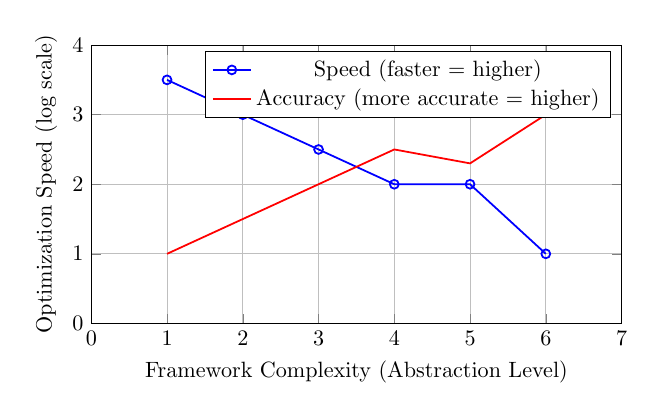
\begin{tikzpicture}[scale=0.8]
\begin{axis}[
xlabel=Framework Complexity (Abstraction Level),
ylabel=Optimization Speed (log scale),
xmin=0, xmax=7,
ymin=0, ymax=4,
grid=major,
width=10cm,
height=6cm,
]
\addplot[blue, mark=o, thick] coordinates {
(1, 3.5)
(2, 3.0)
(3, 2.5)
(4, 2.0)
(5, 2.0)
(6, 1.0)
};
\addlegendentry{Speed (faster = higher)}

\addplot[red, mark=s, thick] coordinates {
(1, 1.0)
(2, 1.5)
(3, 2.0)
(4, 2.5)
(5, 2.3)
(6, 3.0)
};
\addlegendentry{Accuracy (more accurate = higher)}
\end{axis}
\end{tikzpicture}
\caption{Framework Trade-Off: Speed vs Accuracy}
\label{fig:20-speed-accuracy-tradeoff}
\end{figure}

\subsection{Decision Rule: Which Optimization Approach?}

\begin{enumerate}
\item \textbf{Budget <CHF 100k, Timeline <4 weeks:} Use Framework 1 + Exhaustive Search. Speed essential.
\item \textbf{Budget CHF 100-500k, Timeline 2-3 months, homogeneous population:} Use Framework 1 or 2 + Greedy. Balance.
\item \textbf{Budget CHF 100-500k, heterogeneous population, time permits:} Use Framework 4 + Two-Stage. Best ROI.
\item \textbf{Budget >CHF 500k, crisis-prone domain, continuous monitoring:} Use Framework 6 + Adaptive. Max complexity, max reward.
\item \textbf{Unsure about context:} Start with Framework 1 (fast), learn with Framework 4 (mid-scale), graduate to Framework 6 (full-scale) as data/resources grow.
\end{enumerate}

%%%%%%%%%%%%%%%%%%%%%%%%%%%%%%%%%%%%%%%%%%%%%%%%%%%%%%%%%%%%%%%%%%%%%%%%%%%%%%%
\section{Formal Portfolio Optimization: Mathematical Foundations}
\label{sec:20-formal-optimization}
%%%%%%%%%%%%%%%%%%%%%%%%%%%%%%%%%%%%%%%%%%%%%%%%%%%%%%%%%%%%%%%%%%%%%%%%%%%%%%%

Gegeben eine Menge verfügbarer Interventionen, wie wählen wir das optimale Portfolio? (Formale mathematische Behandlung)

\subsection{Das Optimierungsproblem}

\begin{definition}[Portfolio Optimization Problem]
\label{def:20-optimization}
\begin{align}
\max_{P \subseteq \mathcal{I}} \quad & E(P) = \sum_{i \in P} E_i + \sum_{i < j} \gamma_{ij} \sqrt{E_i E_j} \label{eq:20-objective}\\
\text{s.t.} \quad & \sum_{i \in P} c_i \leq B \quad \text{(Budget-Constraint)} \label{eq:20-budget}\\
& C(P) \geq 0.75 \quad \text{(Coherence-Constraint)} \label{eq:20-coherence-constraint}\\
& |P| \leq K \quad \text{(Complexity-Constraint)} \label{eq:20-complexity}
\end{align}
\end{definition}

\subsection{Lösungsalgorithmen}

\textbf{Für kleine Portfolios ($|P| \leq 5$):} Exhaustive Search über alle $\binom{n}{k}$ Kombinationen

\textbf{Für mittlere Portfolios ($5 < |P| \leq 15$):} Greedy Selection mit Coherence-Check

\begin{algorithm}[H]
\caption{Greedy Portfolio Construction}
\label{alg:20-greedy}
\begin{algorithmic}[1]
\State $P \leftarrow \emptyset$
\While{Budget verfügbar \textbf{and} $|P| < K$}
    \State $\mathcal{I}^* \leftarrow \arg\max_{\mathcal{I} \notin P} \Delta E(P \cup \{\mathcal{I}\})$ subject to $C(P \cup \{\mathcal{I}\}) \geq 0.75$
    \If{$\mathcal{I}^*$ exists}
        \State $P \leftarrow P \cup \{\mathcal{I}^*\}$
    \Else
        \State \textbf{break}
    \EndIf
\EndWhile
\State \Return $P$
\end{algorithmic}
\end{algorithm}

\textbf{Für große Portfolios ($|P| > 15$):} Genetische Algorithmen oder Multi-Objective Optimization


%%%%%%%%%%%%%%%%%%%%%%%%%%%%%%%%%%%%%%%%%%%%%%%%%%%%%%%%%%%%%%%%%%%%%%%%%%%%%%%
\subsection{Portfolio-Archetypen: Vordefinierte Optimierungsziele}
\label{sec:20-archetypes}
%%%%%%%%%%%%%%%%%%%%%%%%%%%%%%%%%%%%%%%%%%%%%%%%%%%%%%%%%%%%%%%%%%%%%%%%%%%%%%%

In der Praxis designen wir \textbf{nicht ein Portfolio, sondern mehrere Varianten} zum Vergleich. Die folgenden sieben Archetypen decken die häufigsten strategischen Anforderungen ab \citep{hummel2019effective, szaszi2018systematic}. Die empirische Grundlage für Portfolio-Optimierung stammt aus Meta-Analysen mit über 100 Studien, die mittlere Effektstärken von $d = 0.43$ für Nudges dokumentieren \citep{hummel2019effective}. Die ROI-Überlegenheit von verhaltensbasierten Portfolios gegenüber traditionellen Interventionen (100x--1000x) ist durch Benartzi et al.\ belegt \citep{benartzi2017should}.

\subsubsection{Die Sieben Portfolio-Archetypen}

\begin{table}[htbp]
\centering
\caption{Portfolio-Archetypen: Optimierungsziele und Charakteristiken}
\label{tab:20-archetypes}
\renewcommand{\arraystretch}{1.4}
\footnotesize
\begin{tabular}{@{}llp{3.8cm}ll@{}}
\toprule
\textbf{Archetyp} & \textbf{Fokus} & \textbf{Typische Typen} & \textbf{Constraint} & \textbf{Trade-off} \\
\midrule
\textbf{🚀 Quick Wins} & Schnelle Umsetzung & A1, A2, A3 & Zeit $\leq$ 4 Wochen & Moderate $E$, sofort \\
\textbf{⭐ Optimal Mix} & Max.\ Effektivität & A5, A6, A8 + kompl. & $C(P) \geq 0.85$ & Höchste $E$, aufwändig \\
\textbf{💰 Budget-Constrained} & Beste $E$ pro € & A1, A2, A3 & Cost $\leq B$ & ROI maximiert \\
\textbf{🛡️ Low-Risk} & Min.\ Backfire & A1, A2 (keine A7!) & $\gamma_{ij} \geq 0.1$ & Sicher, konservativ \\
\textbf{🔄 Sustainable} & Langfristige Wirkung & A5, A8 & Scope $\geq$ identity & Langsam, dauerhaft \\
\textbf{📈 Max Behavior Change} & Max.\ $P(\text{BC})$ & Alle + Synergien & $E(P|\vec{S}_0)$ max & Ressourcenintensiv \\
\textbf{🌱 Eco-Sustainable} & Min.\ $d_X$ Impact & A1, A3, A5 (keine A7) & $\Delta d_X \geq 0$ & Ökologisch positiv \\
\bottomrule
\end{tabular}
\end{table}

\subsubsection{Archetyp-Definitionen}

\begin{tcolorbox}[colback=blue!5!white, colframe=blue!75!black,
    title=\textbf{Archetyp 1: 🚀 Quick Wins Portfolio}]
\textbf{Ziel:} Schnellstmögliche, sichtbare Verhaltensänderung mit minimaler Vorlaufzeit.

\textbf{Optimierungsproblem:}
\begin{equation}
\max_{P} E(P) \quad \text{s.t.} \quad \text{TimeToImplement}(P) \leq 4 \text{ Wochen}, \quad |P| \leq 3
\end{equation}

\textbf{Typische Interventionen:}
\begin{itemize}[nosep]
\item A1 (Awareness): Info-Kampagne, E-Mail-Serie
\item A2 (Feedback): Dashboard, Echtzeit-Metriken
\item A3 (Contextual): Default-Änderungen, Opt-out statt Opt-in
\end{itemize}

\textbf{Erwartetes $E$:} 15--25\% (ohne Synergien: 12--18\%)
\end{tcolorbox}

\begin{tcolorbox}[colback=yellow!5!white, colframe=yellow!75!black,
    title=\textbf{Archetyp 2: ⭐ Optimal Mix Portfolio}]
\textbf{Ziel:} Maximale Portfolio-Effektivität unter voller Nutzung aller Synergien.

\textbf{Optimierungsproblem:}
\begin{equation}
\max_{P} \left[ \sum_{i \in P} E_i + \sum_{i<j} \gamma_{ij} \sqrt{E_i E_j} \right] \quad \text{s.t.} \quad C(P) \geq 0.85
\end{equation}

\textbf{Typische Interventionen:}
\begin{itemize}[nosep]
\item A5 (Identity): Rollen-Definition, Selbstkonzept
\item A6 (Social): Normen, Peer Recognition
\item A8 (Commitment): Pre-Commitment, Zielsetzung
\item + A1 oder A3 als Verstärker
\end{itemize}

\textbf{Erwartetes $E$:} 35--50\% (Synergie-Beitrag: 8--15pp)
\end{tcolorbox}

\begin{tcolorbox}[colback=green!5!white, colframe=green!75!black,
    title=\textbf{Archetyp 3: 💰 Budget-Constrained Portfolio}]
\textbf{Ziel:} Maximaler ROI bei begrenztem Budget.

\textbf{Optimierungsproblem:}
\begin{equation}
\max_{P} \frac{E(P)}{\text{Cost}(P)} \quad \text{s.t.} \quad \sum_{i \in P} c_i \leq B
\end{equation}

\textbf{Selektion nach $E_i / c_i$ (Effektivität pro €):}
\begin{center}
\begin{tabular}{@{}lcc@{}}
\toprule
\textbf{Typ} & \textbf{$E_i / c_i$} & \textbf{Priorität} \\
\midrule
A3 (Defaults) & Hoch & 1 \\
A1 (Information) & Mittel-Hoch & 2 \\
A2 (Feedback) & Mittel & 3 \\
A5 (Identity) & Niedrig (aber nachhaltig) & 4 \\
\bottomrule
\end{tabular}
\end{center}

\textbf{Erwartetes $E$:} 20--35\% bei 50\% des Optimal-Budgets
\end{tcolorbox}

\begin{tcolorbox}[colback=red!5!white, colframe=red!75!black,
    title=\textbf{Archetyp 4: 🛡️ Low-Risk Portfolio}]
\textbf{Ziel:} Minimales Backfire-Risiko, keine negativen Überraschungen.

\textbf{Optimierungsproblem:}
\begin{equation}
\max_{P} E(P) \quad \text{s.t.} \quad \gamma_{ij} \geq 0.1 \; \forall i,j, \quad P(\text{Backfire}) < 5\%
\end{equation}

\textbf{Ausgeschlossene Kombinationen:}
\begin{itemize}[nosep]
\item ❌ A6 + A7 (Crowding-out Risiko)
\item ❌ A7 + A8 (Intrinsic Undermining)
\item ❌ A7 alleine bei Social-Oriented Segment
\end{itemize}

\textbf{Sichere Kombinationen:}
\begin{itemize}[nosep]
\item ✅ A1 + A2 + A3 (Information-Feedback-Architecture)
\item ✅ A1 + A5 (Awareness + Identity)
\end{itemize}

\textbf{Erwartetes $E$:} 15--25\% mit $<5\%$ Backfire-Wahrscheinlichkeit
\end{tcolorbox}

\begin{tcolorbox}[colback=purple!5!white, colframe=purple!75!black,
    title=\textbf{Archetyp 5: 🔄 Sustainable Portfolio}]
\textbf{Ziel:} Langfristige, selbstverstärkende Verhaltensänderung (Habit-Formation).

\textbf{Optimierungsproblem:}
\begin{equation}
\max_{P} E(P, t \to \infty) \quad \text{s.t.} \quad \text{Scope}(\mathcal{I}_i) \geq \text{identity} \; \forall i \in P
\end{equation}

\textbf{Typische Interventionen:}
\begin{itemize}[nosep]
\item A5 (Identity): ``Ich bin jemand, der...'' Framing
\item A8 (Commitment): Öffentliche Selbstverpflichtung
\item A3 (Contextual): Umgebungs-Redesign für Gewohnheitsbildung
\end{itemize}

\textbf{Zeithorizont:} 6--18 Monate bis volle Wirkung, dann selbsttragend

\textbf{Erwartetes $E$:} Initial 10--15\%, nach 12 Monaten 30--40\% (ohne weitere Kosten)
\end{tcolorbox}

\begin{tcolorbox}[colback=orange!5!white, colframe=orange!75!black,
    title=\textbf{Archetyp 6: 📈 Maximum Behavior Change Portfolio}]
\textbf{Ziel:} Höchstmögliche Verhaltensänderungs-Wahrscheinlichkeit $P(\text{BC})$.

\textbf{Optimierungsproblem:}
\begin{equation}
\max_{P} P(\text{BC} | \vec{S}_0, P) = \sigma\left( E(P | \vec{S}_0) \right)
\end{equation}

\textbf{Strategie:} Alle 10C-Dimensionen gezielt adressieren:

\begin{center}
\footnotesize
\begin{tabular}{@{}lll@{}}
\toprule
\textbf{10C} & \textbf{Target} & \textbf{Intervention} \\
\midrule
AWARE & $A_0 \to A_1$ & A1 (Information) \\
READY & $W_0 \to W_1$ & A2 (Feedback) + A4 (Temporal) \\
STAGE & $\varphi_0 \to \varphi_1$ & A3 (Contextual) + A4 (Timing) \\
WHO & $\lambda_L$ max & Level-konsistente Interventionen \\
HOW & $\gamma_{ij}$ max & Synergetische Kombinationen \\
\bottomrule
\end{tabular}
\end{center}

\textbf{Erwartetes $P(\text{BC})$:} 45--65\% (vs.\ 15--25\% bei Quick Wins)

\textbf{Kosten:} 3--5× Quick Wins, aber 2--3× Effektivität
\end{tcolorbox}

\begin{tcolorbox}[colback=green!10!white, colframe=green!75!black,
    title=\textbf{Archetyp 7: 🌱 Eco-Sustainable Portfolio}]
\textbf{Ziel:} Verhaltensänderung mit positivem ökologischen Fußabdruck.

\textbf{Optimierungsproblem:}
\begin{equation}
\max_{P} E(P) \quad \text{s.t.} \quad \Delta d_X(P) \geq 0, \quad \text{kein A7 mit negativem } d_X
\end{equation}

\textbf{Ökologisch positive Interventionen:}
\begin{itemize}[nosep]
\item A1 (Digital Information): E-Mail, App-Benachrichtigungen (kein Papier)
\item A3 (Contextual): Default auf nachhaltige Option
\item A5 (Identity): ``Ich bin umweltbewusst'' Framing
\end{itemize}

\textbf{Zu vermeiden:}
\begin{itemize}[nosep]
\item ❌ A7 (Financial) mit materiellen Incentives (Gadgets, Geschenke)
\item ❌ Print-Kampagnen, physische Mailings
\item ❌ Reisen für Face-to-Face Interventionen
\end{itemize}

\textbf{FEPSDE-Fokus:} Dimension X (Ecological) als primäres KPI

\textbf{Erwartetes $E$:} 20--30\% mit $\Delta d_X > 0$
\end{tcolorbox}

\subsubsection{Portfolio-Vergleichs-Matrix}

Die folgende Matrix ermöglicht den direkten Vergleich der Archetypen:

\begin{table}[htbp]
\centering
\caption{Portfolio-Archetypen Vergleichs-Matrix}
\label{tab:20-archetype-comparison}
\renewcommand{\arraystretch}{1.3}
\footnotesize
\begin{tabular}{@{}lccccccc@{}}
\toprule
\textbf{Dimension} & \textbf{🚀 Quick} & \textbf{⭐ Optimal} & \textbf{💰 Budget} & \textbf{🛡️ Safe} & \textbf{🔄 Sust.} & \textbf{📈 Max BC} & \textbf{🌱 Eco} \\
\midrule
$E(P)$ erwartet & 20\% & 45\% & 30\% & 20\% & 35\% & 55\% & 25\% \\
Kosten (relativ) & 1× & 4× & 1.5× & 1.2× & 2× & 5× & 1.5× \\
Zeit bis Wirkung & 2-4 W & 3-6 M & 4-8 W & 2-4 W & 6-18 M & 3-6 M & 4-8 W \\
Backfire-Risiko & Niedrig & Mittel & Niedrig & Minimal & Niedrig & Mittel & Minimal \\
Nachhaltigkeit & Kurz & Mittel & Kurz & Kurz & Hoch & Mittel & Hoch \\
ROI (kurz) & ★★★ & ★★ & ★★★★ & ★★★ & ★ & ★★ & ★★★ \\
ROI (lang) & ★★ & ★★★★ & ★★★ & ★★ & ★★★★★ & ★★★★ & ★★★★ \\
\bottomrule
\end{tabular}
\end{table}

\subsubsection{Entscheidungsbaum für Archetyp-Wahl}

\begin{center}
\begin{tikzpicture}[
    decision/.style={diamond, draw, fill=yellow!20, text width=4em, text badly centered, inner sep=1pt},
    block/.style={rectangle, draw, fill=blue!10, text width=5em, text centered, rounded corners},
    line/.style={draw, -latex'},
    scale=0.85, transform shape
]
\node [decision] (q1) {Budget limitiert?};
\node [block, below left=1.5cm and 2cm of q1] (budget) {💰 Budget};
\node [decision, below right=1.5cm and 0.5cm of q1] (q2) {Zeit kritisch?};
\node [block, below left=1.5cm and 0.5cm of q2] (quick) {🚀 Quick Wins};
\node [decision, below right=1.5cm and 0.5cm of q2] (q3) {Risiko-avers?};
\node [block, below left=1.5cm and 0.5cm of q3] (safe) {🛡️ Low-Risk};
\node [decision, below right=1.5cm and 0.5cm of q3] (q4) {Langfristig?};
\node [block, below left=1.5cm and 0.5cm of q4] (sust) {🔄 Sustainable};
\node [decision, below right=1.5cm and 0.5cm of q4] (q5) {Öko-Fokus?};
\node [block, below left=1.5cm and 0.5cm of q5] (eco) {🌱 Eco};
\node [block, below right=1.5cm and 0.5cm of q5] (maxbc) {📈 Max BC / ⭐ Optimal};

\path [line] (q1) -| node [near start, above] {Ja} (budget);
\path [line] (q1) -- node [near start, right] {Nein} (q2);
\path [line] (q2) -| node [near start, above] {Ja} (quick);
\path [line] (q2) -- node [near start, right] {Nein} (q3);
\path [line] (q3) -| node [near start, above] {Ja} (safe);
\path [line] (q3) -- node [near start, right] {Nein} (q4);
\path [line] (q4) -| node [near start, above] {Ja} (sust);
\path [line] (q4) -- node [near start, right] {Nein} (q5);
\path [line] (q5) -| node [near start, above] {Ja} (eco);
\path [line] (q5) -- node [near start, right] {Nein} (maxbc);
\end{tikzpicture}
\end{center}


%%%%%%%%%%%%%%%%%%%%%%%%%%%%%%%%%%%%%%%%%%%%%%%%%%%%%%%%%%%%%%%%%%%%%%%%%%%%%%%
\subsection{FEPSDE-KPI-Framework: Messung über alle Utility-Dimensionen}
\label{sec:20-fepsde-kpi}
%%%%%%%%%%%%%%%%%%%%%%%%%%%%%%%%%%%%%%%%%%%%%%%%%%%%%%%%%%%%%%%%%%%%%%%%%%%%%%%

Jede Intervention beeinflusst eine oder mehrere der \textbf{sechs FEPSDE-Dimensionen} (aus Appendix UNMAPPED_C, CORE-WHAT). Für den Erfolgsnachweis benötigen wir \textbf{dimensionsspezifische KPIs}. Die KPI-Auswahl basiert auf Meta-Analysen, die type-spezifische Effektstärken dokumentieren: Defaults $d = 0.68$, Feedback $d = 0.41$, Salience $d = 0.29$, Social Norms $d = 0.38$ \citep{mertens2022choice}. Für Scaling-Effekte (Pilot $\to$ National) ist ein Decay-Faktor von 0.3--0.5 zu berücksichtigen \citep{soman2020successfully}.

\begin{table}[htbp]
\centering
\caption{FEPSDE-KPI-Framework: Metriken für alle Utility-Dimensionen}
\label{tab:20-fepsde-kpi}
\renewcommand{\arraystretch}{1.4}
\footnotesize
\begin{tabular}{@{}clp{5cm}p{4cm}@{}}
\toprule
\textbf{Dim.} & \textbf{Dimension} & \textbf{Primäre KPIs} & \textbf{Sekundäre KPIs} \\
\midrule
\textbf{F} & Financial &
\begin{itemize}[nosep, leftmargin=*]
\item Revenue/CLV Impact
\item Conversion Rate Δ
\item Cost Savings
\item Margin Improvement
\end{itemize} &
\begin{itemize}[nosep, leftmargin=*]
\item Payback Period
\item NPV der Intervention
\item Break-even Point
\end{itemize} \\
\midrule
\textbf{E} & Emotional &
\begin{itemize}[nosep, leftmargin=*]
\item NPS (Net Promoter Score)
\item CSAT (Customer Satisfaction)
\item Engagement Score
\item Sentiment Score
\end{itemize} &
\begin{itemize}[nosep, leftmargin=*]
\item Emotionale Valenz (Survey)
\item Brand Attachment Index
\item Frustration Indicators
\end{itemize} \\
\midrule
\textbf{P} & Physical &
\begin{itemize}[nosep, leftmargin=*]
\item Usage Frequency
\item Adoption Rate
\item Behavioral Consistency
\item Habit Strength Index
\end{itemize} &
\begin{itemize}[nosep, leftmargin=*]
\item Time-to-First-Use
\item Feature Utilization
\item Physical Activity Metrics
\end{itemize} \\
\midrule
\textbf{S} & Social &
\begin{itemize}[nosep, leftmargin=*]
\item Referral Rate
\item Social Sharing Count
\item Community Participation
\item Peer Influence Score
\end{itemize} &
\begin{itemize}[nosep, leftmargin=*]
\item Network Effects Multiplier
\item Viral Coefficient
\item Social Proof Indicators
\end{itemize} \\
\midrule
\textbf{D} & Development &
\begin{itemize}[nosep, leftmargin=*]
\item Skill Acquisition Rate
\item Learning Completion \%
\item Competency Growth
\item Career Progression
\end{itemize} &
\begin{itemize}[nosep, leftmargin=*]
\item Knowledge Retention
\item Transfer-to-Practice Rate
\item Self-Efficacy Score
\end{itemize} \\
\midrule
\textbf{X} & Ecological &
\begin{itemize}[nosep, leftmargin=*]
\item Carbon Footprint Δ
\item Resource Consumption Δ
\item Waste Reduction \%
\item Sustainability Score
\end{itemize} &
\begin{itemize}[nosep, leftmargin=*]
\item Energy Efficiency Gain
\item Circular Economy Index
\item Biodiversity Impact
\end{itemize} \\
\bottomrule
\end{tabular}
\end{table}

\subsubsection{KPI-Zuordnung nach Interventionstyp}

\begin{table}[htbp]
\centering
\caption{Interventionstyp → FEPSDE-Dimension → Primäre KPIs}
\label{tab:20-type-kpi-mapping}
\renewcommand{\arraystretch}{1.3}
\footnotesize
\begin{tabular}{@{}llll@{}}
\toprule
\textbf{Typ} & \textbf{Primäre $d$} & \textbf{Sekundäre $d$} & \textbf{Kern-KPIs} \\
\midrule
A1 (Awareness) & P, E & D & Adoption Rate, Sentiment \\
A2 (Feedback) & P, D & E & Usage Frequency, Skill Growth \\
A3 (Contextual) & P, F & E & Conversion Rate, Habit Strength \\
A4 (Temporal) & P, F & E & Time-to-Action, Deadline Compliance \\
A5 (Identity) & E, S & D & NPS, Community Participation \\
A6 (Social) & S, E & P & Referral Rate, Peer Influence \\
A7 (Financial) & F & P & Revenue Impact, Margin \\
A8 (Commitment) & P, D & E & Behavioral Consistency, Goal Achievement \\
\bottomrule
\end{tabular}
\end{table}

\subsubsection{KPI-Messprotokoll für Portfolios}

\begin{tcolorbox}[colback=yellow!5!white, colframe=yellow!75!black,
    title=\textbf{Das 3×3 KPI-Protokoll}]

\textbf{Für jede Intervention im Portfolio:}

\begin{enumerate}
\item \textbf{Vor Intervention ($t_0$):}
   \begin{itemize}[nosep]
   \item Baseline für alle relevanten FEPSDE-Dimensionen messen
   \item $\vec{S}_0$ dokumentieren (10C Status Quo)
   \end{itemize}

\item \textbf{Während Intervention ($t_1$ bis $t_n$):}
   \begin{itemize}[nosep]
   \item Kontinuierliches Tracking der P-Dimension (Behavioral Metrics)
   \item Pulse-Checks für E-Dimension (Engagement)
   \end{itemize}

\item \textbf{Nach Intervention ($t_{\text{end}}$ + 3/6/12 Monate):}
   \begin{itemize}[nosep]
   \item Alle 6 FEPSDE-Dimensionen messen
   \item $\Delta\vec{S}$ berechnen (10C Delta)
   \item Long-term Sustainability prüfen
   \end{itemize}
\end{enumerate}

\textbf{Formel für Multi-Dimensional Success Score:}
\begin{equation}
\text{Success}(P) = \sum_{d \in \text{FEPSDE}} w_d \cdot \frac{\Delta \text{KPI}_d}{\text{Target}_d}
\end{equation}

Wobei $w_d$ die Gewichtung der Dimension (aus dem Business-Kontext) angibt.
\end{tcolorbox}


%%%%%%%%%%%%%%%%%%%%%%%%%%%%%%%%%%%%%%%%%%%%%%%%%%%%%%%%%%%%%%%%%%%%%%%%%%%%%%%
\section{Operational Deployment: From Theory to Practice}
\label{sec:20-deployment}
%%%%%%%%%%%%%%%%%%%%%%%%%%%%%%%%%%%%%%%%%%%%%%%%%%%%%%%%%%%%%%%%%%%%%%%%%%%%%%%

\textbf{Central Challenge:} You've optimized a portfolio using one of the 6 frameworks, passed all 6 sanity checks, and secured budget approval. Now what? How do you actually deploy it and ensure it works as predicted?

\subsection{Pre-Deployment Checklist}

Before deployment, verify these 10 items:

\begin{table}[htbp]
\centering
\caption{Pre-Deployment Checklist}
\label{tab:20-deployment-checklist}
\renewcommand{\arraystretch}{1.3}
\small
\begin{tabular}{@{}llll@{}}
\toprule
\textbf{\#} & \textbf{Item} & \textbf{Verification} & \textbf{Responsible} \\
\midrule
\textbf{1} & Framework Choice & Decision rule (Sec. \ref{subsec:20-decision-tree}) & Technical Lead \\
\midrule
\textbf{2} & Sanity Checks & All 6 Checks pass (Sec. \ref{sec:20-validation}) & QA Lead \\
\midrule
\textbf{3} & Stakeholder Buy-in & Practitioner + Leadership sign-off & Program Manager \\
\midrule
\textbf{4} & Data Infrastructure & Tracking system ready; APIs tested & Data Engineer \\
\midrule
\textbf{5} & Staff Training & Practitioners trained on portfolio logic & HR / Training \\
\midrule
\textbf{6} & Segment/Phase IDs & Classifier trained, validated on pilot & Data Science \\
\midrule
\textbf{7} & Monitoring Dashboard & Real-time E, C(P), Checks 1-6 visible & Analytics \\
\midrule
\textbf{8} & Pilot Results & Small-scale test (n=100--500) passes & Program Manager \\
\midrule
\textbf{9} & Contingency Plan & Fallback if E misses -20\% of target & Program Manager \\
\midrule
\textbf{10} & Budget Buffer & 20\% contingency reserve allocated & Finance \\
\bottomrule
\end{tabular}
\end{table}

\subsection{Deployment Phases: Rollout Strategy}

\textbf{Recommended: Phased Rollout}

\begin{enumerate}
\item \textbf{Phase Alpha (Week 1--2):} Pilot group $n = 100--500$, intensive monitoring, daily check-ins
  \begin{itemize}[nosep]
  \item Expected: E = target ±30\% (large variance is OK)
  \item Red flag: E < 0 or Check 2/3 fails → pause, debug
  \item Go/no-go decision: E > 50\% of target
  \end{itemize}

\item \textbf{Phase Beta (Week 3--6):} Expanded pilot $n = 1,000--5,000$, weekly check-ins, framework adjustment
  \begin{itemize}[nosep]
  \item Expected: E = target ±20\%
  \item Red flag: E drops >15\% from Alpha → likely context shift or segment classification drift
  \item Adjustment: If Framework 3/4/6 (data-dependent), re-train classifiers
  \end{itemize}

\item \textbf{Phase Gamma (Week 7+):} Full rollout $n = $ full population, monthly check-ins, continuous learning
  \begin{itemize}[nosep]
  \item Expected: E converges to target ±10\%
  \item Red flag: E remains >15\% below target after week 12 → portfolio redesign needed
  \end{itemize}

\end{enumerate}

\subsection{Real-Time Monitoring: The Deployment Dashboard}

Deploy a real-time dashboard displaying 12 metrics:

\begin{table}[htbp]
\centering
\caption{Deployment Monitoring Dashboard}
\label{tab:20-deployment-dashboard}
\renewcommand{\arraystretch}{1.3}
\footnotesize
\begin{tabular}{@{}llllll@{}}
\toprule
\textbf{\#} & \textbf{Metric} & \textbf{Update} & \textbf{Target} & \textbf{Red Flag} & \textbf{Action} \\
\midrule
\textbf{1} & $E$ (Effectiveness) & Daily & Target ±5\% & E < 0.8×Target & Debug \\
\midrule
\textbf{2} & $C(P)$ (Coherence) & Daily & $\geq 0.75$ & C < 0.60 & Restart \\
\midrule
\textbf{3} & Participation Rate & Daily & 80\%+ & <60\% & Comms boost \\
\midrule
\textbf{4} & Dropout Rate & Daily & <5\% & >10\% & Check UX \\
\midrule
\textbf{5} & Segment Drift & Weekly & $|\Delta P(s|\text{data})|<0.05$ & >0.15 & Re-classify \\
\midrule
\textbf{6} & Phase Transition & Weekly & Expected flow & Bottleneck & Remove friction \\
\midrule
\textbf{7} & Context Indicator $\Psi$ & Weekly & Stable & Shift >0.5σ & Adapt portfolio \\
\midrule
\textbf{8} & Check 1 (Agg) & Weekly & KL <0.15 & >0.25 & Review clusters \\
\midrule
\textbf{9} & Check 2 (Segment) & Weekly & ≤1 segment off & ≥4 off & Redesign \\
\midrule
\textbf{10} & Check 4 (γ) & Weekly & $\gamma_{ij} > -0.1$ & $< -0.2$ & Remove pair \\
\midrule
\textbf{11} & Check 5 (Phase) & Weekly & ≥2 phases α>0.7 & 0 phases & Change timing \\
\midrule
\textbf{12} & Budget Spend vs Plan & Weekly & On-target & >20\% variance & Adjust spend \\
\bottomrule
\end{tabular}
\end{table}

\subsection{Adaptive Adjustment Rules}

If metrics exceed red-flag thresholds, trigger these automated or semi-automated adjustments:

\begin{definition}[Adaptive Adjustment Logic]

\begin{enumerate}
\item \textbf{If $E < 0.8 \times \text{Target}$:}
  \begin{itemize}[nosep]
  \item Check 1: Run Sanity Check 1 (aggregation). If fails → reduce complexity (move to simpler Framework)
  \item Check 2: Run Sanity Check 2 (segment). If 2+ segments off → add segment-specific adaptation (upgrade to Framework 4)
  \item Check 3: Run Sanity Check 3 (context). If Ψ-sensitivity >0.5 → activate context-adaptive rules (upgrade to Framework 6)
  \item Check 5: Run Sanity Check 5 (phase). If any phase α<0.5 → add phase-specific intervention
  \end{itemize}

\item \textbf{If Dropout Rate >10\%:}
  \begin{itemize}[nosep]
  \item Qualitative interviews with drop-outs (n=20-50)
  \item Likely cause: UX friction, low motivation, privacy concerns, perceived fairness
  \item Response options: Simplify UX, increase salience, add autonomy cue, improve transparency
  \end{itemize}

\item \textbf{If Segment Drift $|\Delta P(s|\text{data})|>0.15$:}
  \begin{itemize}[nosep]
  \item Re-train segment classifier (if Framework 4/6 dependent on classification)
  \item Possible cause: Population composition changed, economic conditions shifted, behavior patterns evolved
  \item Response: Re-estimate segment posteriors; possibly adjust portfolio composition
  \end{itemize}

\item \textbf{If Context Shift Ψ moves >0.5σ:}
  \begin{itemize}[nosep]
  \item For Framework 6: Automatically adjust portfolio via context-sensitivity formula
  \item For Frameworks 1-5: Manual re-optimization. Possible cause: Crisis, major shock
  \item Response: Escalate to Program Manager for decision on stay-course vs adapt
  \end{itemize}

\end{enumerate}

\end{definition}

\subsection{Learning Loop: Feedback into Continuous Improvement}

\textbf{Monthly Learning Cycle:}

\begin{enumerate}
\item \textbf{Week 1: Aggregate Data}
  \begin{itemize}[nosep]
  \item Compute actual E, C(P), all 12 dashboard metrics
  \item Compare to predictions from Ch17-19 continuous model
  \item Compute residual: $\text{Residual} = E_{\text{actual}} - E_{\text{predicted}}$
  \end{itemize}

\item \textbf{Week 2: Root-Cause Analysis}
  \begin{itemize}[nosep]
  \item If Residual >±15\%, investigate via 6 Sanity Checks
  \item Which Check failed? What changed?
  \item Hypothesis: Aggregation error? Segment shift? Context change? Complementarity backfire?
  \end{itemize}

\item \textbf{Week 3: Parameter Update}
  \begin{itemize}[nosep]
  \item If segment σ-values differ from literature: Update local $\sigma(s, \mathcal{I})$ matrix
  \item If phase α-values shift: Update local $\alpha(\varphi, I)$ matrix
  \item If γ-complementarity differs: Update local $\gamma_{ij}$ matrix
  \item Repository: Store in parameter files with timestamp versioning
  \end{itemize}

\item \textbf{Week 4: Adjustment & Replication}
  \begin{itemize}[nosep]
  \item Adjust portfolio for next month based on learnings
  \item Document changes: What was updated, why, what effect expected?
  \item Replicate to similar populations if parameters generalizable
  \end{itemize}

\end{enumerate}

\subsection{End-of-Deployment Report Template}

After 3-6 months of deployment, prepare a structured end-of-deployment report:

\begin{table}[htbp]
\centering
\caption{End-of-Deployment Report Sections}
\label{tab:20-deployment-report}
\small
\begin{tabular}{@{}lll@{}}
\toprule
\textbf{Section} & \textbf{Key Outputs} & \textbf{Audience} \\
\midrule
\textbf{Executive Summary} & E achieved, C(P), ROI, 1-2 key learnings & Leadership \\
\midrule
\textbf{Portfolio Performance} & E by framework, by segment, by phase & Technical \\
\midrule
\textbf{Sanity Checks Results} & All 6 checks: pass/fail, residuals & Technical \\
\midrule
\textbf{Parameter Learnings} & Updated σ, α, γ values; confidence intervals & Data Science \\
\midrule
\textbf{Segment \& Phase Insights} & Drift, new patterns, subgroups discovered & Program \\
\midrule
\textbf{Context Effects} & Ψ stability, context-sensitivity actual vs predicted & Strategic \\
\midrule
\textbf{Failures \& Debugging} & Which interventions underperformed, why & Practitioner \\
\midrule
\textbf{Scaling Recommendation} & Go/no-go for full-scale rollout & Program Manager \\
\midrule
\textbf{Next-Phase Improvements} & Framework upgrade (e.g., 1→4), new segments, novel interventions & Strategy \\
\bottomrule
\end{tabular}
\end{table}

\subsection{Success Criteria for Deployment}

\textbf{Minimum Success:} E $\geq 0.85 \times$ Target, C(P) $\geq 0.75$, Dropout $\leq 15\%$

\textbf{Good Success:} E $\geq 0.95 \times$ Target, C(P) $\geq 0.80$, Dropout $\leq 8\%$

\textbf{Excellent Success:} E $\geq 1.0 \times$ Target, C(P) $\geq 0.85$, Dropout $\leq 5\%$, Learnings incorporated into next cycle

%%%%%%%%%%%%%%%%%%%%%%%%%%%%%%%%%%%%%%%%%%%%%%%%%%%%%%%%%%%%%%%%%%%%%%%%%%%%%%%
\section{Multi-Level Implementation}
\label{sec:20-levels}
%%%%%%%%%%%%%%%%%%%%%%%%%%%%%%%%%%%%%%%%%%%%%%%%%%%%%%%%%%%%%%%%%%%%%%%%%%%%%%%

Portfolios müssen für verschiedene Implementierungs-Level angepasst werden.

\subsection{Die Sechs Implementierungs-Level}

\begin{table}[htbp]
\centering
\caption{Charakteristiken der Implementierungs-Level}
\label{tab:20-levels}
\renewcommand{\arraystretch}{1.4}
\small
\begin{tabular}{@{}lllll@{}}
\toprule
\textbf{Level} & \textbf{Akteure} & \textbf{Portfolio-Fokus} & \textbf{Zeithorizont} & \textbf{$n$} \\
\midrule
L1: Individual & Coach, Therapeut & Habit + Mikro-Environment & Wochen & 1 \\
L2: Household & Familie, Berater & Rollen + Ressourcen & Monate & 2--5 \\
L3: Organization & HR, Management & Struktur + Kultur + Incentives & 1--3 Jahre & 50--5000 \\
L4: Region & Regierung, Industrie & Bildung + Infrastruktur & 5--15 Jahre & 10k--1M \\
L5: Nation & Parlament, Gerichte & Institutionen + Normen & 10--30 Jahre & 1M--100M \\
L6: Global & UN, WTO, Koalitionen & Treaties + Enforcement & Dekaden & 1B+ \\
\bottomrule
\end{tabular}
\end{table}

\subsection{Level-spezifische Portfolio-Prinzipien}

\begin{enumerate}
\item \textbf{L1-L2 (Mikro):} Hohe Personalisierung, kurze Feedback-Loops, adaptive Anpassung
\item \textbf{L3 (Meso):} Balance zwischen Standardisierung und Segment-Targeting
\item \textbf{L4-L6 (Makro):} Institutionelle Verankerung, lange Zeithorizonte, Policy-Bundles
\end{enumerate}

\subsection{Cross-Level Coherence}

\begin{theorem}[Cross-Level Coherence]
\label{thm:20-cross-level}
Portfolios auf verschiedenen Levels sollten kohärent sein:
\begin{equation}
\gamma_{L_i, L_j} \geq 0 \quad \forall \, L_i, L_j
\label{eq:20-cross-level}
\end{equation}
Interventionen auf Level $L_i$ sollten Interventionen auf Level $L_j$ nicht unterminieren.
\end{theorem}

\textbf{Beispiel Konflikt:} Organisationale Incentives (L3) können nationale Norm-Kampagnen (L5) unterminieren, wenn sie Crowding-out auslösen.


%%%%%%%%%%%%%%%%%%%%%%%%%%%%%%%%%%%%%%%%%%%%%%%%%%%%%%%%%%%%%%%%%%%%%%%%%%%%%%%
\section{Hierarchical Portfolio Optimization}
\label{sec:20-hierarchical}
%%%%%%%%%%%%%%%%%%%%%%%%%%%%%%%%%%%%%%%%%%%%%%%%%%%%%%%%%%%%%%%%%%%%%%%%%%%%%%%

Neben den \textbf{Implementierungs-Leveln} (L1--L6) aus Section~\ref{sec:20-levels} gibt es eine orthogonale Dimension: die \textbf{Entscheidungshierarchie}. Diese unterscheidet, \textit{auf welcher Ebene} Portfolio-Entscheidungen getroffen werden.

\begin{tcolorbox}[colback=blue!5!white, colframe=blue!75!black,
    title=\textbf{Die drei Entscheidungsebenen}]

\textbf{Strategisch (High-Level):}
\begin{itemize}[nosep]
\item \textbf{Was:} Gesamtrichtung, Priorisierung der 10C-Dimensionen, Segment-Reihenfolge
\item \textbf{Horizont:} 3--12 Jahre
\item \textbf{Fragen:} ``Welche Dimensionen priorisieren?'' ``Welche Segmente zuerst?''
\item \textbf{Output:} Gewichteter Portfolio-Vektor $\vec{I}_{\text{weighted}}$, Segment-Sequenz, Modul-Kombinationen
\item \textbf{Entscheider:} Programmleitung, Policy-Maker
\end{itemize}

\textbf{Taktisch (Mid-Level):}
\begin{itemize}[nosep]
\item \textbf{Was:} Konkrete Kampagnen, Kanal-Wahl, Botschaften pro Segment
\item \textbf{Horizont:} 3--24 Monate
\item \textbf{Fragen:} ``Welche Kampagnen?'' ``Welche Kanäle?'' ``Welche Messages pro Segment?''
\item \textbf{Output:} Kampagnen-Portfolio, Kanal-Allocation, Quartals-KPIs
\item \textbf{Entscheider:} Kampagnen-Manager, Projektleitung
\end{itemize}

\textbf{Operativ (Ground-Level):}
\begin{itemize}[nosep]
\item \textbf{Was:} Konkrete Touchpoints, Materialien, Interaktionen, Trigger-Response
\item \textbf{Horizont:} 1 Tag -- 3 Monate
\item \textbf{Fragen:} ``Was passiert bei Trigger-Event?'' ``Wie sieht der Content aus?''
\item \textbf{Output:} Scripts, Content Assets, Response-Protokolle, AB-Tests
\item \textbf{Entscheider:} Ausführungsteam, Content-Manager
\end{itemize}

\end{tcolorbox}

\begin{table}[htbp]
\centering
\caption{Mapping: Entscheidungsebenen $\leftrightarrow$ EIT-EMP-3 Scope Levels (Chapter 11)}
\label{tab:20-scope-mapping}
\renewcommand{\arraystretch}{1.4}
\small
\begin{tabular}{@{}llccc@{}}
\toprule
\textbf{Chapter 20} & \textbf{EIT-EMP-3} & \textbf{$K^*$ Adj.} & \textbf{$\alpha$-Affinity} & \textbf{Typische Mechanismen} \\
\midrule
--- & L0 (Systemic) & ×0.6 & Infrastructure, Policy & Institutionelle Verankerung \\
Strategisch & L1 (Strategic) & ×0.8 & Identity, Commitment & Langfrist-Programme \\
Taktisch & L2 (Program) & ×1.0 & Social, Incentive & Kampagnen, Quartals-KPIs \\
Operativ & L3 (Operational) & ×1.2 & Nudge, Reminder & Touchpoints, Scripts \\
(Instant) & L4 (Instant) & ×1.5 & Prompt, Salience & Trigger-Response \\
\bottomrule
\end{tabular}

\vspace{0.2cm}
\footnotesize
\textit{Quelle: Chapter 11, §11.20.3 (EIT-EMP-3 Scope Level Emergence); Appendix UNMAPPED_IE (EMERGE-SPEC)}
\end{table}

\textbf{Interpretation:} Die Entscheidungsebenen in Chapter 20 entsprechen direkt den EIT-EMP-3 Scope Levels. Jedes Level hat einen spezifischen $K^*$-Adjustment-Faktor: Systemische Interventionen (L0) erfordern größeren Fokus ($K^* \times 0.6$), während Instant-Interventionen (L4) mehr parallele Maßnahmen erlauben ($K^* \times 1.5$).

\subsection{Temporale Dimensionen}
\label{sec:20-temporal-dimensions}

Orthogonal zur Entscheidungshierarchie stehen die \textbf{temporalen Horizonte}:

\begin{table}[htbp]
\centering
\caption{Temporale Dimensionen und anwendbare Entscheidungsebenen}
\label{tab:20-temporal-dimensions}
\renewcommand{\arraystretch}{1.4}
\small
\begin{tabular}{@{}llll@{}}
\toprule
\textbf{Horizont} & \textbf{Zeitraum} & \textbf{Anwendbare Ebenen} & \textbf{Typische Use Cases} \\
\midrule
\textbf{Instant} & $< 24$h & Operativ & Trigger-Response, Anfragen \\
\textbf{Kurzfristig} & 1 Woche -- 3 Monate & Operativ, Taktisch & Kampagnen-Wellen, AB-Tests \\
\textbf{Mittelfristig} & 3--12 Monate & Taktisch, Strategisch & Jahres-Plan, Segment-Entwicklung \\
\textbf{Langfristig} & 1--12 Jahre & Strategisch & Gesamtstrategie, Norm-Veränderung \\
\bottomrule
\end{tabular}
\end{table}

\subsection{Die Optimierungs-Matrix (Ebene $\times$ Temporal)}
\label{sec:20-optimization-matrix}

Die Kreuzung von Entscheidungsebenen und Zeithorizonten ergibt eine \textbf{Optimierungs-Matrix}, wobei jede Zelle spezifische Optimierungsziele und KPIs hat:

\begin{table}[htbp]
\centering
\caption{Optimierungs-Matrix: Entscheidungsebene $\times$ Zeithorizont}
\label{tab:20-optimization-matrix}
\renewcommand{\arraystretch}{1.5}
\small
\begin{tabular}{@{}l|llll@{}}
\toprule
& \textbf{Instant} & \textbf{Kurzfristig} & \textbf{Mittelfristig} & \textbf{Langfristig} \\
\midrule
\textbf{Strategisch} & --- & Quick Wins & Penetration & Systemshift \\
& & (First Response) & (Marktdurchdringung) & ($\Delta W_{\text{base}}$, $\Delta\kappa$) \\
\midrule
\textbf{Taktisch} & Trigger-Response & Kampagnen & Conversion & --- \\
& (Response Time) & (CPL) & (Rate/Segment) & \\
\midrule
\textbf{Operativ} & Touchpoint & Content & --- & --- \\
& (CSAT, Quality) & (CTR, Engagement) & & \\
\bottomrule
\end{tabular}
\end{table}

\subsection{Constraint-basierte Portfolio-Optimierung}
\label{sec:20-constraint-optimization}

Das hierarchische Optimierungsproblem unterliegt sechs Klassen von \textbf{Nebenbedingungen}:

\begin{definition}[Hierarchical Portfolio Optimization Problem]
\label{def:20-hierarchical-optimization}
\begin{align}
\max_{P_{\text{str}}, P_{\text{tac}}, P_{\text{op}}} \quad & \sum_{s \in \text{Segments}} \sum_{m \in \text{Modules}} w_{sm} \cdot E[\Delta W_{sm}(\vec{I}_{sm})] \label{eq:20-hierarchical-obj}\\
\text{s.t.} \quad & \text{C1: Budget} \quad \sum_i \text{cost}(I_i) \leq B_{\text{total}} \label{eq:20-c1}\\
& \text{C2: Crowding} \quad \gamma(I_i, I_j) \geq \gamma_{\min} \quad \forall i,j \in P \label{eq:20-c2}\\
& \text{C3: Timing} \quad t(I_i) < t(I_j) \text{ wenn } I_i \rightarrow I_j \label{eq:20-c3}\\
& \text{C4: Capacity} \quad \sum \text{cap\_required} \leq \text{cap\_available} \label{eq:20-c4}\\
& \text{C5: Ethical} \quad \text{autonomy}(I_i) \geq \eta_{\min} \label{eq:20-c5}\\
& \text{C6: Segment} \quad \sigma(I_i, S_j) \geq \sigma_{\min} \label{eq:20-c6}\\
& \text{C7: K-Optimal} \quad |P| \leq K^*(\text{budget}, \text{complexity}, \text{stage}, \text{crowding}, \text{scope}) \label{eq:20-c7}
\end{align}
\end{definition}

\textbf{NEU --- C7 K-Optimal Constraint (EIT-EMP-2, EXC-3 Hybrid):} Die optimale Portfolio-Größe $K^*$ ist \textbf{nicht frei wählbar}, sondern emergiert aus fünf Faktoren. Per \textbf{Exclusion Principle (EXC-3)} ist nur $f_B$ multiplikativ (Veto-Logik: $B=0 \Rightarrow K^*=0$):
\begin{equation}
K^* = K_{\text{base}} \cdot f_B + \delta_C + \delta_S + \delta_\gamma + \delta_L
\label{eq:20-k-optimal}
\end{equation}
wobei:
\begin{itemize}[nosep]
\item $f_B = \sqrt{B/B_{\text{ref}}}$ --- Budget-Faktor (\textbf{MULTIPLIKATIV}: $B=0 \Rightarrow K^*=0$)
\item $\delta_C = -0.2 \cdot K_{\text{base}} \cdot (c - c_{\text{ref}})$ --- Komplexitäts-Adjustment (\textbf{ADDITIV})
\item $\delta_S = K_{\text{base}} \cdot (\alpha_{BCJ} - 1)$ --- BCJ-Phase-Adjustment (\textbf{ADDITIV})
\item $\delta_\gamma = -K_{\text{base}} \cdot |\bar{\gamma}_{\text{neg}}|$ --- Crowding-Adjustment (\textbf{ADDITIV})
\item $\delta_L = 0.1 \cdot K_{\text{base}} \cdot (L - 1)$ --- Scope-Level-Adjustment (\textbf{ADDITIV})
\end{itemize}
\textit{Begründung: Appendix UNMAPPED_FRM, Axiom EXC-3 (Hybrid Formulation).}
\textit{Implementation: Chapter 11, Section 11.20; \texttt{python scripts/emerge\_algorithm.py}}

\subsubsection{Die sechs Constraint-Klassen im Detail}

\begin{enumerate}
\item \textbf{C1 Budget-Constraint:} Gesamtbudget wird auf strategische, taktische und operative Aktivitäten aufgeteilt:
\begin{equation}
B_{\text{strategic}} + B_{\text{tactical}} + B_{\text{operative}} = B_{\text{total}}
\end{equation}

\item \textbf{C2 Crowding-Out Constraint:} Bekannte Konflikte vermeiden:
\begin{itemize}[nosep]
\item $\gamma(\text{Social}, \text{Financial}) = -0.2$: Finanzielle Anreize untergraben soziale Normen
\item $\gamma(\text{Financial}, \text{Intrinsic}) = -0.3$: Externe Belohnungen untergraben intrinsische Motivation
\end{itemize}
$\Rightarrow$ Konfligierende Interventionen nicht simultan, sondern sequentiell oder separiert

\item \textbf{C3 Timing-Constraint:} Reihenfolge-Abhängigkeiten:
\begin{itemize}[nosep]
\item $I_{\text{AWARE}} \prec I_{\text{WHAT}}$: Erst Awareness, dann Motivation
\item $I_{\text{WHAT}} \prec I_{\text{WHEN}}$: Erst Motivation, dann Choice Architecture
\item $I_{\text{AWARE}} \prec I_{\text{READY}}$: Wissen vor Handlungsbereitschaft
\end{itemize}

\item \textbf{C4 Kapazitäts-Constraint:} Engpässe berücksichtigen (Installateure, Berater, Verarbeitung)

\item \textbf{C5 Ethik-Constraint:} Autonomie-Score $\geq \eta_{\min}$:
\begin{itemize}[nosep]
\item Prohibiert: Mandate ohne Option, Deception, Exploitative Framing
\item Required: Transparenz, Opt-out bei Defaults
\end{itemize}

\item \textbf{C6 Segment-Eignung Constraint:} $\sigma(I, S) \geq \sigma_{\min}$ für Segment $S$:
\begin{itemize}[nosep]
\item Backfire-Risiko: $\sigma < 0$ muss dokumentiert werden
\item Segment-Ausschlüsse: z.B.\ keine mandate\_individual für Gruppen ohne Entscheidungsautonomie
\end{itemize}

\item \textbf{C7 K-Optimal Constraint (NEU):} Portfolio-Größe begrenzt durch $K^*$:
\begin{itemize}[nosep]
\item $|P| \leq K^*$: Anzahl Interventionen darf $K^*$ nicht überschreiten
\item $K^*$ emergiert aus 5 Faktoren (siehe Eq.~\ref{eq:20-k-optimal})
\item \textbf{Scope-Adjustment:} L0 (×0.6) $\to$ L4 (×1.5) gemäß Table~\ref{tab:20-scope-mapping}
\item Verhindert Über-Komplexität und Ressourcen-Streuung
\end{itemize}
\end{enumerate}

\subsection{Hierarchischer Workflow: Von Strategie zu Operation}
\label{sec:20-hierarchical-workflow}

\begin{tcolorbox}[colback=green!5!white, colframe=green!75!black,
    title=\textbf{Der hierarchische Optimierungs-Workflow}]

\begin{enumerate}
\item \textbf{Strategische Ebene (jährlich) --- EIT-EMP-3 Level L1:}
\begin{itemize}[nosep]
\item Input: 10C Status Quo $\vec{S}_0$, Verhaltensparameter $\Theta$, Kontext $\Psi$
\item Optimierung: $\max E[\Delta W]$ unter C1--C7 mit $K^*_{\text{L1}} = K_{\text{base}} \times 0.8$
\item Output: $\vec{I}_{\text{weighted}}$, Segment-Sequenz, Modul-Prioritäten
\item \textit{Typisch: 3--5 strategische Interventionen}
\end{itemize}

\item \textbf{Taktische Ebene (quartalsweise) --- EIT-EMP-3 Level L2:}
\begin{itemize}[nosep]
\item Input: Strategische Vorgaben, Budget-Allocation, Segment-Fokus
\item Optimierung: $\max \text{Conversion}$ unter C1--C4, C7 mit $K^*_{\text{L2}} = K_{\text{base}} \times 1.0$
\item Output: Kampagnen-Portfolio $\{K_1, ..., K_n\}$, Kanal-Mix, KPIs
\item \textit{Typisch: 5--8 taktische Kampagnen pro Quartal}
\end{itemize}

\item \textbf{Operative Ebene (wöchentlich) --- EIT-EMP-3 Level L3:}
\begin{itemize}[nosep]
\item Input: Taktische Vorgaben, Trigger-Events, Feedback
\item Optimierung: $\max \text{Response Rate}$ unter C4--C7 mit $K^*_{\text{L3}} = K_{\text{base}} \times 1.2$
\item Output: Touchpoint-Scripts, Content, AB-Test-Varianten
\item \textit{Typisch: 8--12 parallele operative Maßnahmen}
\end{itemize}
\end{enumerate}

\textbf{Feedback-Loop:} Operative Ergebnisse $\rightarrow$ Taktische Anpassung $\rightarrow$ Strategische Review

\textbf{$K^*$-Kaskade:} $K^*_{\text{L1}} \leq K^*_{\text{L2}} \leq K^*_{\text{L3}}$ --- höhere Granularität erlaubt mehr parallele Interventionen

\end{tcolorbox}

\subsection{Beispiel: Energie-Effizienz-Kampagne (BFE)}
\label{sec:20-hierarchical-example}

\begin{table}[htbp]
\centering
\caption{Hierarchische Portfolio-Optimierung: BFE Energie Schweiz für Private}
\label{tab:20-bfe-example}
\renewcommand{\arraystretch}{1.4}
\small
\begin{tabular}{@{}llll@{}}
\toprule
\textbf{Ebene} & \textbf{Entscheidung} & \textbf{Output} & \textbf{KPI} \\
\midrule
\textbf{Strategisch} & 10C-Priorisierung: & $I_{\text{AWARE}}: 0.30$ & Fossil$\rightarrow$Erneuerbar \\
(3--12 Jahre) & AWARE $>$ WHAT $>$ WHEN & $I_{\text{WHAT}}: 0.25$ & Quote +10pp \\
& Segment: EFH $\rightarrow$ MFH $\rightarrow$ STWE & $I_{\text{WHEN}}: 0.20$ & \\
\midrule
\textbf{Taktisch} & 3 Kampagnen Q1/2027: & Heizungs-Check (CHF 80k) & Leads: 5500 \\
(3--24 Monate) & - Heizungs-Check Februar & Förder-Offensive (CHF 70k) & Conversion: 35\% \\
& - Förder-Offensive März & Solar-Start (CHF 50k) & CPL: CHF 90 \\
& - Solar-Frühlingsstart April & & \\
\midrule
\textbf{Operativ} & Trigger-Response: & Installateur-Toolkit & Response $<$ 24h \\
(1 Tag -- 3 Mon.) & - Bei Heizungsdefekt & Sofort-Beratung & CSAT $\geq$ 4.5 \\
& - Nach Impulsberatung & Sanierungsfahrplan & \\
\bottomrule
\end{tabular}
\end{table}

\textbf{Constraint-Prüfung:}
\begin{itemize}[nosep]
\item C1 Budget: CHF 500k = 10\% strategisch + 40\% taktisch + 50\% operativ \checkmark
\item C2 Crowding: Keine simultane Social + Financial Aktivierung \checkmark
\item C3 Timing: AWARE $\prec$ WHAT $\prec$ WHEN Sequenz \checkmark
\item C4 Capacity: Beratungskapazität skalierbar \checkmark
\item C5 Ethical: Alle Interventionen transparent, Opt-out möglich \checkmark
\item C6 Segment: EFH-optimierte Interventionen \checkmark
\end{itemize}


%%%%%%%%%%%%%%%%%%%%%%%%%%%%%%%%%%%%%%%%%%%%%%%%%%%%%%%%%%%%%%%%%%%%%%%%%%%%%%%
\section{Simulation und Prediction}
\label{sec:20-simulation}
%%%%%%%%%%%%%%%%%%%%%%%%%%%%%%%%%%%%%%%%%%%%%%%%%%%%%%%%%%%%%%%%%%%%%%%%%%%%%%%

Vor Implementation werden Portfolio-Effekte simuliert. Dieser Abschnitt formalisiert, wie der \textbf{10C Status Quo Vektor} in die \textbf{Vorhersage der Verhaltensänderung} eingeht.

\subsection{10C-basierte Vorhersage der Verhaltensänderung}
\label{sec:20-9c-prediction}

\begin{tcolorbox}[colback=blue!5!white, colframe=blue!75!black,
    title=\textbf{KRITISCH: Die 10C → Prediction Pipeline}]

\textbf{Das fehlende Glied:} Der Status Quo Vektor $\vec{S}_0$ (aus Kapitel 17) muss in die Portfolio-Effektivitäts-Formel $E(P)$ eingehen, um die \textbf{Wahrscheinlichkeit der Verhaltensänderung} zu berechnen.

\end{tcolorbox}

\subsubsection{Von $\vec{S}_0$ zur Vorhersage}

Gegeben der 10C Status Quo Vektor:
\begin{equation}
\vec{S}_0 = (L, d, \gamma_{\text{current}}, \Psi, \Theta, A_0, W_0, \varphi_0, \text{Scope})
\end{equation}

Und ein Interventions-Portfolio $P = \{\mathcal{I}_1, ..., \mathcal{I}_n\}$, berechnet sich die \textbf{erwartete Verhaltensänderung} als:

\begin{tcolorbox}[colback=green!5!white, colframe=green!75!black,
    title=\textbf{Definition: 10C-basierte Verhaltensänderungs-Vorhersage}]
\begin{equation}
\boxed{P(\text{BC} | \vec{S}_0, P) = f\left( E(P | \vec{S}_0) \right) = \sigma\left( \beta_0 + \beta_1 \cdot E(P | \vec{S}_0) \right)}
\label{eq:20-bc-prediction}
\end{equation}

Wobei $E(P | \vec{S}_0)$ die \textbf{bedingte Portfolio-Effektivität} ist:
\begin{equation}
\boxed{E(P | \vec{S}_0) = \sum_{i \in P} E_{\max,i} \cdot \underbrace{\alpha_{t_i,\varphi_0}}_{\text{aus STAGE}} \cdot \underbrace{\sigma_{s(A_0, W_0)}}_{\text{aus AWARE/READY}} \cdot \underbrace{\lambda_L}_{\text{aus WHO}} \cdot \underbrace{\gamma(\Psi)}_{\text{aus WHEN}} + \sum_{i<j} \gamma_{ij} \cdot \sqrt{E_i E_j}}
\label{eq:20-e-conditional}
\end{equation}
\end{tcolorbox}

\subsubsection{10C-Dimensionen in der Formel}

\begin{table}[htbp]
\centering
\caption{Wie jede 10C-Dimension in die Vorhersage eingeht}
\label{tab:20-9c-to-prediction}
\renewcommand{\arraystretch}{1.4}
\footnotesize
\begin{tabular}{@{}llll@{}}
\toprule
\textbf{10C CORE} & \textbf{$\vec{S}_0$-Komponente} & \textbf{Formel-Parameter} & \textbf{Effekt auf $E(P)$} \\
\midrule
\textbf{WHO} (AAA) & $L \in \{1,2,3,4\}$ & $\lambda_L$ & Level-Multiplikator \\
\textbf{WHAT} (C) & $d \subseteq \{F,E,P,S,D,X\}$ & $E_{\max,i}(d)$ & Dimension-Passung \\
\textbf{HOW} (B) & $\gamma_{\text{current}}$ & $\gamma_{ij}$ (additiv) & Synergie-Verstärkung \\
\textbf{WHEN} (V) & $\Psi$ & $\gamma(\Psi)$ & Kontext-Modulation \\
\textbf{WHERE} (BBB) & $\Theta$ & Prior für $\theta_n$ & Parameter-Unsicherheit \\
\textbf{AWARE} (AU) & $A_0$ & $s(A_0, \cdot)$ & Segment-Zuweisung \\
\textbf{READY} (AV) & $W_0$ & $s(\cdot, W_0)$ & Segment-Zuweisung \\
\textbf{STAGE} (AW) & $\varphi_0$ & $\alpha_{t,\varphi_0}$ & Phase-Type Affinity \\
\textbf{HIERARCHY} (HI) & Scope & $\tau_{\text{decay}}$ & Effekt-Persistenz \\
\bottomrule
\end{tabular}
\end{table}

\subsubsection{Der vollständige Berechnungs-Workflow}

\begin{enumerate}
\item \textbf{Input: 10C Status Quo Assessment} (aus Kapitel 17, Sec. 0)
\begin{equation}
\vec{S}_0 = (L=2, d=\{F,E\}, \gamma_{\text{current}}=0, \Psi=\Psi_{\text{workplace}}, \Theta_{\text{lit}}, A_0=0.4, W_0=0.3, \varphi_0=2, \text{tactical})
\end{equation}

\item \textbf{Segment-Zuweisung} aus $(A_0, W_0)$:
\begin{equation}
s(\vec{S}_0) = \begin{cases}
\text{present\_biased} & \text{wenn } A_0 > 0.5 \text{ und } W_0 < 0.4 \\
\text{naif} & \text{wenn } A_0 < 0.3 \\
\text{sophisticate} & \text{wenn } A_0 > 0.7 \text{ und } W_0 > 0.6 \\
... & ...
\end{cases}
\end{equation}

\item \textbf{Phase-Type Affinity} aus $\varphi_0$:
\begin{equation}
\alpha_{t_i, \varphi_0=2} = \text{(aus Phase-Type Affinity Matrix, Kapitel 18)}
\end{equation}

\item \textbf{Kontext-Modulation} aus $\Psi$:
\begin{equation}
\gamma(\Psi_{\text{workplace}}) = \text{(aus Appendix UNMAPPED_V, CORE-WHEN)}
\end{equation}

\item \textbf{Portfolio-Effektivität berechnen}:
\begin{equation}
E(P | \vec{S}_0) = \sum_{i} E_i \cdot \alpha_{t_i, 2} \cdot \sigma_{s} \cdot \lambda_2 \cdot \gamma(\Psi) + \sum_{i<j} \gamma_{ij} \sqrt{E_i E_j}
\end{equation}

\item \textbf{Verhaltensänderungs-Wahrscheinlichkeit}:
\begin{equation}
P(\text{BC} | \vec{S}_0, P) = \sigma(E(P | \vec{S}_0)) \quad \text{(Logistische Transformation)}
\end{equation}
\end{enumerate}

\begin{tcolorbox}[colback=yellow!5!white, colframe=yellow!75!black,
    title=\textbf{Worked Example: Von $\vec{S}_0$ zu $P(\text{BC})$}]

\textbf{Gegeben:}
\begin{itemize}[nosep]
\item $\vec{S}_0$: $L=2$, $A_0=0.35$, $W_0=0.25$, $\varphi_0=1$ (Awareness), Workplace-Kontext
\item Portfolio: $P = \{$A1: Info-Kampagne, A3: Default-Opt-In$\}$
\end{itemize}

\textbf{Berechnung:}
\begin{enumerate}[nosep]
\item Segment: $s = \text{naif}$ (wegen $A_0 < 0.4$)
\item Phase-Type Affinity: $\alpha_{A1, \varphi=1} = 0.9$, $\alpha_{A3, \varphi=1} = 0.3$
\item Segment-Multiplier: $\sigma_{\text{naif}, A1} = 0.8$, $\sigma_{\text{naif}, A3} = 1.4$
\item Basis-Effektivität: $E_{\text{A1}} = 0.12$, $E_{\text{A3}} = 0.18$
\item Synergie: $\gamma_{A1,A3} = +0.4$
\end{enumerate}

\textbf{Ergebnis:}
\begin{align}
E(P | \vec{S}_0) &= 0.12 \cdot 0.9 \cdot 0.8 + 0.18 \cdot 0.3 \cdot 1.4 + 0.4 \cdot \sqrt{0.12 \cdot 0.18} \nonumber \\
&= 0.086 + 0.076 + 0.059 = 0.221 \quad (22.1\%)
\end{align}

\textbf{Empfehlung:} A3 (Default) erst in Phase 2 (Triggered) einsetzen, da $\alpha_{A3, \varphi=1} = 0.3$ suboptimal ist.
\end{tcolorbox}

\subsection{Der Simulations-Workflow}

\begin{enumerate}
\item \textbf{Input-Spezifikation:}
   \begin{itemize}[nosep]
   \item Intervention-Tuples aus HHH 20-Field Schema
   \item $\gamma_{ij}$-Schätzungen aus Appendix UNMAPPED_REG
   \item Segment-Verteilung der Zielgruppe
   \item Journey-Phase-Verteilung
   \end{itemize}

\item \textbf{Monte Carlo Simulation:}
\begin{equation}
\hat{E}(P) = \frac{1}{N} \sum_{n=1}^{N} E(P | \theta_n), \quad \theta_n \sim \text{Prior}(\theta)
\label{eq:20-monte-carlo}
\end{equation}
wobei $\theta$ die unsicheren Parameter ($\gamma_{ij}$, $\alpha_{t,\varphi}$, $\sigma_s$) sind.

\item \textbf{Sensitivitätsanalyse:}
   \begin{itemize}[nosep]
   \item Welche $\gamma_{ij}$ haben größten Einfluss?
   \item Was passiert bei Fehl-Schätzung?
   \item Break-even Analyse
   \end{itemize}

\item \textbf{Output:}
\begin{equation}
\hat{E}(P) = 18.5\% \pm 3.2\% \quad [95\% \text{ CI}: 12.3\%, 24.7\%]
\label{eq:20-simulation-output}
\end{equation}
\end{enumerate}

\subsection{Risiko-Metriken}

\begin{itemize}
\item \textbf{P(Negative Outcome):} $P(E(P) < 0)$ --- Wahrscheinlichkeit eines Gesamtschadens
\item \textbf{Value at Risk:} $\text{VaR}_{5\%}(E(P))$ --- Worst-case bei 5\% Quantil
\item \textbf{Expected Shortfall:} $E[E(P) | E(P) < \text{VaR}]$ --- Durchschnittlicher Schaden im Worst-case
\end{itemize}


%%%%%%%%%%%%%%%%%%%%%%%%%%%%%%%%%%%%%%%%%%%%%%%%%%%%%%%%%%%%%%%%%%%%%%%%%%%%%%%
\section{Evaluation und Organizational Learning}
\label{sec:20-learning}
%%%%%%%%%%%%%%%%%%%%%%%%%%%%%%%%%%%%%%%%%%%%%%%%%%%%%%%%%%%%%%%%%%%%%%%%%%%%%%%

Portfolios müssen evaluiert werden, um $\gamma$-Schätzungen zu verbessern.

\subsection{Der Drei-Schritt Evaluations-Prozess}

\begin{enumerate}
\item \textbf{Messung (Appendix THL1):}
   \begin{itemize}[nosep]
   \item Pre-registered Outcomes
   \item Kontrollgruppen (wo möglich)
   \item Long-term Follow-up (6--12 Monate)
   \end{itemize}

\item \textbf{Attribution:}
   \begin{itemize}[nosep]
   \item Einzeleffekte isolieren: $\hat{E}(\mathcal{I}_i)$
   \item Interaktionseffekte schätzen: $\hat{\gamma}_{ij}$
   \item Konfidenzintervalle berechnen
   \end{itemize}

\item \textbf{Repository-Update (Appendix UNMAPPED_REG):}
\begin{equation}
\gamma_{ij}^{\text{new}} = \lambda \cdot \gamma_{ij}^{\text{prior}} + (1-\lambda) \cdot \hat{\gamma}_{ij}^{\text{observed}}
\label{eq:20-bayesian-update}
\end{equation}
wobei $\lambda$ den Gewichtungsfaktor für Prior-Wissen angibt.
\end{enumerate}

\subsection{Der Learning Loop}

\begin{center}
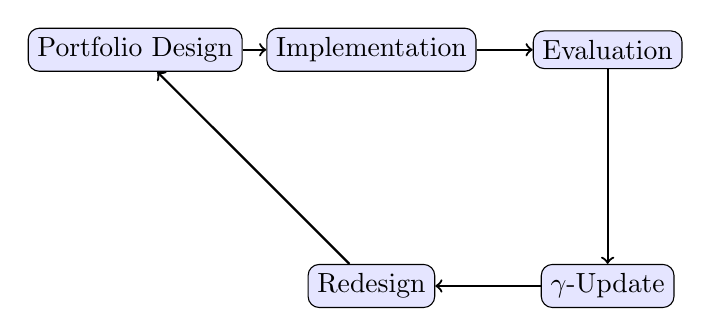
\begin{tikzpicture}[node distance=3cm, auto]
    \node[draw, rounded corners, fill=blue!10] (design) {Portfolio Design};
    \node[draw, rounded corners, fill=blue!10, right of=design] (implement) {Implementation};
    \node[draw, rounded corners, fill=blue!10, right of=implement] (evaluate) {Evaluation};
    \node[draw, rounded corners, fill=blue!10, below of=evaluate] (update) {$\gamma$-Update};
    \node[draw, rounded corners, fill=blue!10, left of=update] (redesign) {Redesign};

    \draw[->, thick] (design) -- (implement);
    \draw[->, thick] (implement) -- (evaluate);
    \draw[->, thick] (evaluate) -- (update);
    \draw[->, thick] (update) -- (redesign);
    \draw[->, thick] (redesign) -- (design);
\end{tikzpicture}
\end{center}

\subsection{Organizational Learning Metriken}

\begin{itemize}
\item \textbf{$\gamma$-Precision:} Reduktion der Konfidenzintervall-Breite über Zeit
\item \textbf{Prediction Accuracy:} $|E_{\text{predicted}} - E_{\text{observed}}|$
\item \textbf{Portfolio Efficiency:} $\frac{E(P)}{Cost(P)}$ über Iterationen
\end{itemize}

\subsection{10C Delta Measurement: Der vollständige Learning Loop}
\label{sec:20-9c-delta}

Das 10C Framework ermöglicht eine \textbf{systematische Messung der Veränderung} durch Interventionen. Kapitel 17 etabliert den \textbf{Status Quo Vektor} $\vec{S}_0$; dieses Kapitel formalisiert den \textbf{Delta Vektor} $\Delta\vec{S}$.

\subsubsection{Der 10C Delta Vektor}

\begin{tcolorbox}[colback=purple!5!white, colframe=purple!75!black,
    title=\textbf{Definition: 10C Delta Measurement}]

Gegeben der Status Quo Vektor vor Intervention (aus Kapitel 17):
\begin{equation}
\vec{S}_0 = (L, d, \gamma_{\text{current}}, \Psi, \Theta, A_0, W_0, \varphi_0, \text{Scope})
\end{equation}

Und der Post-Intervention Zustand $\vec{S}_1$, definieren wir:

\begin{equation}
\boxed{\Delta\vec{S} = \vec{S}_1 - \vec{S}_0 = (\Delta L, \Delta d, \Delta\gamma, \Delta\Psi, \Delta\Theta, \Delta A, \Delta W, \Delta\varphi, \Delta\text{Scope})}
\end{equation}

Wobei jede Dimension spezifisch gemessen wird:
\end{tcolorbox}

\subsubsection{Dimensions-spezifische Messung}

\begin{table}[htbp]
\centering
\caption{10C Delta Measurement: Dimensionen, Metriken und Interventions-Typ}
\label{tab:20-9c-delta-measurement}
\renewcommand{\arraystretch}{1.4}
\footnotesize
\begin{tabular}{@{}llp{4.5cm}l@{}}
\toprule
\textbf{CORE} & \textbf{$\Delta$} & \textbf{Messmethode} & \textbf{Primärer Typ} \\
\midrule
\textbf{WHO} (AAA) & $\Delta L$ & Shift in Welfare-Level (L1→L2→L3→L4) & A5, A6 \\
\textbf{WHAT} (C) & $\Delta d$ & Änderung in FEPSDE-Gewichtung & A5, A7 \\
\textbf{HOW} (B) & $\Delta\gamma$ & Neue Komplementaritäten aktiviert & A8, A3 \\
\textbf{WHEN} (V) & $\Delta\Psi$ & Kontext-Sensitivität verändert & A3, A4 \\
\textbf{WHERE} (BBB) & $\Delta\Theta$ & Parameter-Updates (Bayesian) & Alle \\
\textbf{AWARE} (AU) & $\Delta A$ & $A_1 - A_0$ (0--1 Skala) & A1, A2 \\
\textbf{READY} (AV) & $\Delta W$ & $W_{\text{eff},1} - W_{\text{eff},0}$ & A2, A4 \\
\textbf{STAGE} (AW) & $\Delta\varphi$ & Journey-Phase Progression & A3, A4 \\
\textbf{HIERARCHY} (HI) & $\Delta$Scope & Instant→Identity→Habit Shift & A5, A8 \\
\bottomrule
\end{tabular}
\end{table}

\subsubsection{Quantifizierung des $\Delta$-Vektors}

\textbf{Für kontinuierliche Dimensionen (AU, AV):}
\begin{equation}
\Delta A = A_1 - A_0, \quad \Delta W = W_{\text{eff},1} - W_{\text{eff},0}
\end{equation}

\textbf{Für kategoriale Dimensionen (STAGE, HIERARCHY):}
\begin{equation}
\Delta\varphi = \begin{cases}
+1 & \text{wenn Progression (z.B.\ Awareness → Triggered)} \\
0 & \text{keine Veränderung} \\
-1 & \text{Regression (Relapse)}
\end{cases}
\end{equation}

\textbf{Für Portfolio-Parameter (WHERE):}
\begin{equation}
\Theta_1 = \lambda \cdot \Theta_0 + (1-\lambda) \cdot \hat{\Theta}_{\text{observed}}
\label{eq:20-bayesian-theta-update}
\end{equation}

\subsubsection{Der vollständige Status Quo → Delta → Learning Loop}

\begin{tcolorbox}[colback=green!5!white, colframe=green!75!black,
    title=\textbf{Der 10C Learning Loop (Kapitel 17 → 20 → zurück)}]

\begin{center}
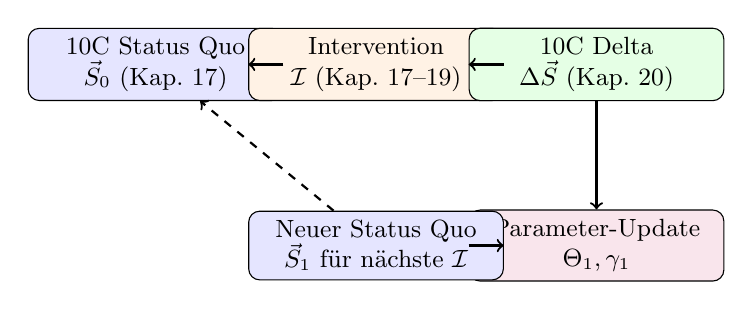
\begin{tikzpicture}[node distance=2.8cm, auto, every node/.style={font=\small}]
    \node[draw, rounded corners, fill=blue!10, text width=3cm, align=center] (status) {10C Status Quo\\$\vec{S}_0$ (Kap.\ 17)};
    \node[draw, rounded corners, fill=orange!10, text width=3cm, align=center, right of=status] (interv) {Intervention\\$\mathcal{I}$ (Kap.\ 17--19)};
    \node[draw, rounded corners, fill=green!10, text width=3cm, align=center, right of=interv] (delta) {10C Delta\\$\Delta\vec{S}$ (Kap.\ 20)};
    \node[draw, rounded corners, fill=purple!10, text width=3cm, align=center, below of=delta, yshift=0.5cm] (learn) {Parameter-Update\\$\Theta_1, \gamma_1$};
    \node[draw, rounded corners, fill=blue!10, text width=3cm, align=center, left of=learn] (newstatus) {Neuer Status Quo\\$\vec{S}_1$ für nächste $\mathcal{I}$};

    \draw[->, thick] (status) -- (interv);
    \draw[->, thick] (interv) -- (delta);
    \draw[->, thick] (delta) -- (learn);
    \draw[->, thick] (learn) -- (newstatus);
    \draw[->, thick, dashed] (newstatus) -- (status);
\end{tikzpicture}
\end{center}

\textbf{Feedback in das 10C System:}
\begin{enumerate}[nosep]
\item $\Delta A, \Delta W$: Updates für $A(\cdot)$ und $W_{\text{eff}}$ Modelle (AU, AV)
\item $\Delta\gamma$: Neue Komplementaritäts-Schätzungen für HOW (B)
\item $\Delta\Theta$: Parameter-Repository (BBB) wird aktualisiert
\item $\Delta\varphi$: Journey-Übergangswahrscheinlichkeiten (AW) verfeinert
\end{enumerate}
\end{tcolorbox}

\subsubsection{Erfolgs-Kriterien für das Portfolio}

\begin{equation}
\text{Portfolio-Erfolg} = \begin{cases}
\text{Vollständig} & \text{wenn } \Delta A > 0, \Delta W > 0, \Delta\varphi \geq 0 \\
\text{Partiell} & \text{wenn mindestens 2 von 3 positiv} \\
\text{Gescheitert} & \text{wenn } \Delta A \leq 0 \text{ und } \Delta W \leq 0
\end{cases}
\end{equation}

\textbf{Interventions-Attribution:} Bei Portfolio $P = \{\mathcal{I}_1, ..., \mathcal{I}_n\}$:
\begin{equation}
\Delta\vec{S} = \sum_{i \in P} \Delta\vec{S}(\mathcal{I}_i) + \text{Interaction Terms}
\end{equation}


%%%%%%%%%%%%%%%%%%%%%%%%%%%%%%%%%%%%%%%%%%%%%%%%%%%%%%%%%%%%%%%%%%%%%%%%%%%%%%%
\section{Worked Examples}
\label{sec:20-examples}
%%%%%%%%%%%%%%%%%%%%%%%%%%%%%%%%%%%%%%%%%%%%%%%%%%%%%%%%%%%%%%%%%%%%%%%%%%%%%%%

\subsection{Beispiel 1: Anna's Kommunales Energie-Portfolio (Vollständig)}

\textbf{Kontext:} Gemeinde mit 10,000 Haushalten, Ziel: -20\% Energieverbrauch, Budget: CHF 200k

\textbf{Schritt 1: Segment-Analyse}
\begin{itemize}[nosep]
\item Present-Biased: 30\%
\item Social-Oriented: 45\%
\item Autonomy-Seeking: 25\%
\end{itemize}

\textbf{Schritt 2: Portfolio-Design}

\begin{table}[htbp]
\centering
\caption{Anna's Energie-Portfolio mit Kohärenz-Check}
\label{tab:20-example-anna}
\renewcommand{\arraystretch}{1.3}
\small
\begin{tabular}{@{}lllcccc@{}}
\toprule
\textbf{Intervention} & \textbf{Typ} & \textbf{Phase} & \textbf{Segment} & \textbf{$E_i$} & \textbf{Kosten} \\
\midrule
$\mathcal{I}_1$: Social Norm Letter & A6 & Awareness & Social & 5\% & CHF 20k \\
$\mathcal{I}_2$: Smart Meter + Feedback & A2+A3 & Action & All & 6\% & CHF 120k \\
$\mathcal{I}_3$: Neighborhood Competition & A6 & Maintenance & Social & 5\% & CHF 40k \\
$\mathcal{I}_4$: Self-Set Goal (Opt-in) & A8 & Trigger & Autonomy & 3\% & CHF 20k \\
\bottomrule
\end{tabular}
\end{table}

\textbf{Schritt 3: Kohärenz-Check}
\begin{itemize}[nosep]
\item C1 (Non-Interference): $\gamma_{12} = +0.5$, $\gamma_{23} = +0.4$, $\gamma_{34} = +0.3$ ✓
\item C2 (Journey-Coverage): Awareness, Trigger, Action, Maintenance ✓
\item C3 (Segment-Coverage): Social + Autonomy + All ✓
\item C4 (Context-Consistency): Alle Haushalt-Kontext ✓
\item \textbf{$C(P) = 1.0$} ✓
\end{itemize}

\textbf{Schritt 4: Effekt-Berechnung}
\begin{align}
E(P) &= (5 + 6 + 5 + 3) + 0.5\sqrt{5 \cdot 6} + 0.4\sqrt{6 \cdot 5} + 0.3\sqrt{5 \cdot 3} + ... \nonumber\\
&= 19\% + 2.7\% + 2.2\% + 1.2\% + 0.8\% = \mathbf{25.9\%}
\label{eq:20-anna-calculation}
\end{align}

\textbf{Ergebnis:} Ziel (-20\%) übertroffen durch Synergie-Effekte.

\subsection{Beispiel 2: Corporate Wellness Portfolio}

\textbf{Kontext:} Unternehmen mit 2,000 Mitarbeitern, Ziel: Gesündere Belegschaft, Budget: CHF 150k

\begin{table}[htbp]
\centering
\caption{Corporate Wellness Portfolio}
\label{tab:20-example-wellness}
\renewcommand{\arraystretch}{1.3}
\small
\begin{tabular}{@{}llll@{}}
\toprule
\textbf{Intervention} & \textbf{Ziel-Segment} & \textbf{Mechanismus} & \textbf{$\gamma$ mit anderen} \\
\midrule
Team Fitness Challenge & Social-Oriented & Peer Pressure + Fun & $+0.5$ mit Feedback \\
Health Dashboard (App) & Present-Biased & Real-time Feedback & $+0.4$ mit Challenge \\
Flexible Wellness Budget & Autonomy-Oriented & Self-Selection & $+0.3$ mit beiden \\
\bottomrule
\end{tabular}
\end{table}

\textbf{Kohärenz-Check:} Keine Crowding-out Risiken (keine A7+A8 Kombination). $C(P) = 0.85$.

\textbf{Erwarteter ROI:} 3.5:1 (basierend auf reduzierter Abwesenheit + Produktivität)

\subsection{Beispiel 3: Nationales Spar-Programm (Multi-Level)}

\textbf{Kontext:} Regierung will nationale Sparquote erhöhen.

\begin{table}[htbp]
\centering
\caption{Multi-Level Spar-Portfolio}
\label{tab:20-example-national}
\renewcommand{\arraystretch}{1.3}
\small
\begin{tabular}{@{}lllc@{}}
\toprule
\textbf{Level} & \textbf{Intervention} & \textbf{Akteur} & \textbf{Zeithorizont} \\
\midrule
L3 (Org) & Auto-Enrollment in Pensionskassen & Arbeitgeber & 1--2 Jahre \\
L4 (Region) & Finanzbildung in Schulen & Kantone & 5--10 Jahre \\
L5 (Nation) & Steuerliche Spar-Anreize & Parlament & 10+ Jahre \\
L5 (Nation) & ``Sparer sind klug''-Kampagne (A5+A6) & Bund & Ongoing \\
\bottomrule
\end{tabular}
\end{table}

\textbf{Cross-Level Kohärenz-Check:}
\begin{itemize}[nosep]
\item L3 Auto-Enrollment + L5 Steuer-Anreize: $\gamma = +0.4$ (verstärken sich)
\item L4 Finanzbildung + L5 Kampagne: $\gamma = +0.5$ (Information + Norm)
\item \textbf{Achtung:} Steuer-Anreize (A7) nicht mit Commitment-Programmen (A8) kombinieren!
\end{itemize}


\subsection{Beispiel 4: HR Retention Portfolio mit Benefits-Komplementarität}
\label{sec:20-example-hr-retention}

\textbf{Kontext:} Ein Unternehmen mit 2,000 Mitarbeitern will die Fluktuation um 30\% reduzieren. Budget für ein kohärentes Interventions-Portfolio.

\textbf{Das Portfolio:}

\begin{table}[htbp]
\centering
\caption{HR Retention Portfolio: 7 Interventionen über alle Phasen}
\label{tab:20-hr-retention}
\renewcommand{\arraystretch}{1.3}
\small
\begin{tabular}{@{}llllc@{}}
\toprule
\textbf{ID} & \textbf{Intervention} & \textbf{Typ} & \textbf{Phase} & \textbf{$\alpha$} \\
\midrule
INT-HR-001 & Career Path Visibility & A1 (Awareness) & Awareness & 0.9 \\
INT-HR-002 & Development Dashboard & A2 (Feedback) & Action, Maint. & 0.9, 0.8 \\
INT-HR-003 & Auto-Enrollment Training & A3 (Contextual) & Triggered, Action & 0.8, 0.9 \\
INT-HR-004 & Retention Bonus & A7a (Financial) & Action & 0.9 \\
INT-HR-005 & Certification Program & A5a (Identity) & Stable & 0.9 \\
INT-HR-006 & Benefits Package & A7b (Financial) & Maintenance & 0.8 \\
INT-HR-007 & Mental Identity Budgets & A5b (Identity) & Stable & 0.9 \\
\bottomrule
\end{tabular}
\end{table}

\textbf{Synergien ($\gamma > 0$):}
\begin{itemize}[nosep]
\item A1 + A3: $\gamma = +0.4$ (Awareness macht Defaults effektiver)
\item A2 + A3: $\gamma = +0.3$ (Feedback verstärkt Kontextänderungen)
\item A1 + A5: $\gamma = +0.2$ (Career Visibility + Identity)
\end{itemize}

\textbf{Crowding-Out Status:} Kein A6 oder A8 im Portfolio $\rightarrow$ keine Crowding-Out Risiken mit A7.

\subsubsection{Benefits-Komplementarität: $\gamma$ zwischen einzelnen Benefits}

Innerhalb von INT-HR-006 (Benefits Package) existieren eigene Komplementaritäten:

\begin{table}[htbp]
\centering
\caption{Benefit-Komplementaritäts-Matrix (Auszug)}
\label{tab:20-benefit-gamma}
\renewcommand{\arraystretch}{1.2}
\small
\begin{tabular}{@{}lcc@{}}
\toprule
\textbf{Benefit-Paar} & \textbf{$\gamma$} & \textbf{Implikation} \\
\midrule
Firmenauto + Parkplatz & $+0.5$ & Immer zusammen anbieten \\
Kinderbetreuung + FlexTime & $+0.4$ & Verstärken Work-Life-Balance \\
Gym + Mental Health & $+0.35$ & Ganzheitliche Gesundheit \\
\midrule
Firmenauto + ÖV-Abo & $-0.3$ & \textbf{Substitute: nur eines!} \\
Essenszuschuss + Kantine & $-0.2$ & Substituieren sich \\
\bottomrule
\end{tabular}
\end{table}

\textbf{Optimierungs-Regel:} Komplementäre Benefits zuerst, Substitute vermeiden.

\subsubsection{Grenznutzen-Analyse für Benefits}

\begin{tcolorbox}[colback=yellow!5!white, colframe=yellow!75!black,
    title=Diminishing Returns bei Benefits]

\textbf{Formel:}
\begin{equation}
MU(n) = MU_{\text{base}} \times (1 - \delta)^{n-1}
\end{equation}

Wobei $MU_{\text{base}} = 0.8$ und $\delta = 0.25$ (typische Werte).

\textbf{Tier-Struktur:}
\begin{center}
\begin{tabular}{@{}lll@{}}
\toprule
\textbf{Tier} & \textbf{MU-Bereich} & \textbf{Beispiele} \\
\midrule
Tier 1 (Essential) & 0.8--1.0 & Gehalt, KV, Pension \\
Tier 2 (Expected) & 0.5--0.8 & FlexTime, Home-Office \\
Tier 3 (Differentiating) & 0.3--0.5 & Kinderbetreuung, Gym \\
Tier 4 (Premium) & 0.15--0.3 & Firmenauto, Private Schule \\
Tier 5 (Luxury) & $<0.1$ & Concierge (kann negativ werden!) \\
\bottomrule
\end{tabular}
\end{center}

\textbf{Stopp-Regel:} Stoppe wenn $MU < 0.2$ (pragmatische Schwelle).
\end{tcolorbox}

\subsubsection{Choice Architecture für Benefits-Auswahl}

\textbf{Forschungsbasis:}
\begin{itemize}[nosep]
\item Miller (1956): $7 \pm 2$ Regel für kognitive Kapazität
\item Iyengar \& Lepper (2000): Weniger Optionen $\rightarrow$ mehr Entscheidungen
\item Schwartz (2004): Paradox of Choice
\end{itemize}

\textbf{Optimale Choice Box:}
\begin{equation}
\text{Zufriedenheit}(n) = Z_{\max} \times (1 - 0.03 \times \max(0, n-7))
\end{equation}

$\Rightarrow$ Jede Option über 7 senkt Zufriedenheit um $\approx 3\%$.

\begin{tcolorbox}[colback=green!5!white, colframe=green!75!black]
\textbf{Empfehlung:}
\begin{itemize}[nosep]
\item Kategorien: 4 (Mobility, Health, Family, Financial)
\item Optionen pro Kategorie: 3 (Good-Better-Best)
\item Total sichtbar: $\leq 12$
\item \textbf{Smart Default} nach Mitarbeiter-Profil (70\%+ nehmen Default!)
\item Änderbar: 1$\times$ jährlich
\end{itemize}
\end{tcolorbox}

\textbf{Ergebnis des HR Retention Portfolios:}
\begin{itemize}[nosep]
\item Alle 5 Journey-Phasen abgedeckt
\item Alle Segmente angesprochen (via Mental Identity Budgets)
\item Keine Crowding-Out Risiken
\item Geschätzte Fluktuations-Reduktion: 25--35\%
\end{itemize}


%%%%%%%%%%%%%%%%%%%%%%%%%%%%%%%%%%%%%%%%%%%%%%%%%%%%%%%%%%%%%%%%%%%%%%%%%%%%%%%
\section{Der Vollständige Interventions-Design-Workflow: Von A nach B}
\label{sec:20-workflow}
%%%%%%%%%%%%%%%%%%%%%%%%%%%%%%%%%%%%%%%%%%%%%%%%%%%%%%%%%%%%%%%%%%%%%%%%%%%%%%%

Der Weg von \textbf{A} (Diagnose) zu \textbf{B} (fertiges Portfolio) ist \textbf{nicht deterministisch}. An jedem Schritt existieren multiple Pfade, die zu unterschiedlichen finalen Portfolios führen. Diese Section legt den vollständigen Workflow offen.

\subsection{Drei Emergenz-Modi: E-Full, E-Partial, E-None}
\label{sec:20-workflow-paths}

\begin{tcolorbox}[colback=red!5!white, colframe=red!75!black,
    title=\textbf{Fundamentale Entscheidung: Welcher Emergenz-Modus?}]

Die zentrale Frage ist nicht ``Pfad A oder B?'', sondern: \textbf{Was lassen wir emergieren vs.\ was setzen wir vorab?} (Siehe Appendix TKT, Section~\ref{sec:hhh-emergence-modes} für vollständige Theorie.)

\begin{center}
\renewcommand{\arraystretch}{1.4}
\begin{tabular}{@{}p{3.5cm}p{4cm}p{4cm}@{}}
\toprule
\textbf{E-Full} & \textbf{E-Partial} & \textbf{E-None} \\
\midrule
Alles emergiert aus $\vec{S}_0$ & $\varphi, \tau$ emergieren; $\gamma$ preset & Nichts emergiert \\
$\vec{I} \in [0,1]^9$ kontinuierlich & Mix: Emergence + Literatur & A1--A8 Cluster \\
$\gamma(\vec{I}_i, \vec{I}_j)$ berechnet & $\gamma_{ij}$ aus BBB & $\gamma_{ij}$ preset \\
\textbf{Maximale Präzision} & \textbf{Balance} & \textbf{Maximale Geschwindigkeit} \\
Forschung, große Projekte & Standard-Praxis & Schnellentscheidungen \\
\bottomrule
\end{tabular}
\end{center}

\textbf{Entscheidung basiert auf Datenverfügbarkeit} (Data Sufficiency Score $D_{\text{suff}}$):
\begin{itemize}[nosep]
\item $D_{\text{suff}} > 0.8$ (Empirisch oder LLMMC) $\Rightarrow$ \textbf{E-Full} empfohlen
\item $0.5 < D_{\text{suff}} \leq 0.8$ (Mix) $\Rightarrow$ \textbf{E-Partial} empfohlen
\item $D_{\text{suff}} < 0.5$ (nur Expert-Schätzung) $\Rightarrow$ \textbf{E-None} oder E-Partial mit breitem CI
\end{itemize}

\textbf{Kritisch:} LLMMC (LLM Monte Carlo) demokratisiert E-Full! Auch ohne teure Surveys ist Emergence möglich.
\end{tcolorbox}

\subsubsection{E-Full: Workflow mit vollständiger Emergenz}

Im \textbf{E-Full Modus} emergiert alles aus $\vec{S}_0$. Phase 4 (Heuristik) entfällt:

\begin{center}
\footnotesize
\fbox{%
$\vec{S}_0 \xrightarrow{\text{Ph.0}}
\varphi, \tau \xrightarrow{\text{Ph.1}}
\sigma_s \xrightarrow{\text{Ph.2}}
\vec{I} \in [0,1]^9 \xrightarrow{\text{Ph.3}}
\gamma(\vec{I}_i, \vec{I}_j) \xrightarrow{\text{Ph.5a}}
P_{\text{opt}} \xrightarrow{\text{Ph.5b}}
C(P) \xrightarrow{\text{Ph.6}}
P^*$%
}
\end{center}

\textbf{Unterschiede zu E-None:}
\begin{enumerate}[nosep]
\item \textbf{Phase 3 Output:} Bleibt als kontinuierlicher Vektor $\vec{I}$, keine Cluster-Zuordnung
\item \textbf{Phase 5a:} $\gamma(\vec{I}_i, \vec{I}_j) = f(d(\vec{I}_i, \vec{I}_j), \text{Mechanismus-Überlappung})$ --- kontinuierlich berechnet
\item \textbf{Phase 5b Optimierung:}
    \begin{equation}
    \max_{\{\vec{I}_1, ..., \vec{I}_n\} \subset [0,1]^9} E(P) = \sum_{i} E(\vec{I}_i) + \sum_{i<j} \gamma(\vec{I}_i, \vec{I}_j) \sqrt{E_i E_j}
    \end{equation}
\item \textbf{Phase 6 Kohärenz:} C1--C4 werden auf kontinuierliche $\vec{I}$-Vektoren angewandt
\end{enumerate}

\textbf{Vorteil:} Keine Informationsverlust durch Diskretisierung; Interventionen können ``zwischen'' Clustern liegen.

\subsubsection{E-None: Workflow mit heuristischen Clustern (A1--A8)}

Im \textbf{E-None Modus} emergiert nichts; Phase 4 (Heuristik) wird eingefügt:

\begin{center}
\footnotesize
\fbox{%
$\vec{S}_0 \xrightarrow{\text{Ph.0}}
\varphi, \tau \xrightarrow{\text{Ph.1}}
\sigma_s \xrightarrow{\text{Ph.2}}
\vec{I} \xrightarrow{\text{Ph.3}}
\boxed{A_k} \xrightarrow{\text{Ph.4}}
\gamma_{ij} \xrightarrow{\text{Ph.5a}}
P_{\text{opt}} \xrightarrow{\text{Ph.5b}}
C(P) \xrightarrow{\text{Ph.6}}
P^*$%
}
\end{center}

\textbf{Phase 4 (Heuristik):} $\vec{I} \mapsto A_k$ via Nearest-Cluster-Assignment:
\begin{equation}
A_k = \arg\min_{k \in \{1,...,8\}} \|\vec{I} - \vec{\mu}_k\|
\end{equation}

\textbf{Vorteil:} Schnellere Entscheidungen; nutzt vorab berechnete $\gamma_{ij}$-Matrix.

\textbf{Nachteil:} Informationsverlust; Interventionen nahe Cluster-Grenzen werden suboptimal behandelt.

\begin{tcolorbox}[colback=yellow!5!white, colframe=yellow!75!black,
    title=\textbf{Wann welchen Emergenz-Modus wählen?}]

\textbf{E-Full} ist obligatorisch, wenn:
\begin{itemize}[nosep]
\item Die Intervention \textbf{nicht} eindeutig einem A1--A8 Cluster zugeordnet werden kann
\item \textbf{Hybride} Interventionen designt werden (z.B.\ ``80\% Feedback + 20\% Social'')
\item Die \textbf{genaue Intensität} jeder Dimension kalibriert werden muss
\item \textbf{Sensitivitätsanalysen} durchgeführt werden sollen
\item \textbf{Forschungsprojekte} mit hohen Genauigkeitsanforderungen
\item $D_{\text{suff}} > 0.7$ (ausreichend Daten für hohe Konfidenz)
\end{itemize}

\textbf{E-Partial} ist empfohlen, wenn:
\begin{itemize}[nosep]
\item $\varphi$ und $\tau$ emergieren sollen, aber $\gamma$ aus Literatur genommen wird
\item Mix aus empirischen Daten und LLMMC-Schätzungen vorliegt
\item $0.4 < D_{\text{suff}} \leq 0.7$
\end{itemize}

\textbf{E-None} ist ausreichend, wenn:
\begin{itemize}[nosep]
\item Interventionen \textbf{prototypisch} sind (klar einem Cluster zuordenbar)
\item \textbf{Zeitdruck} besteht (Entscheidung in $<$ 1 Tag)
\item Die vorhandene $\gamma_{ij}$-Matrix \textbf{validiert} ist für den Kontext
\item $D_{\text{suff}} < 0.4$ (Emergence würde nur ``strukturierte Unsicherheit'' liefern)
\end{itemize}

\end{tcolorbox}

\subsection{Der Workflow als Pipeline (E-None Modus)}
\label{sec:20-workflow-phases}

\begin{tcolorbox}[colback=blue!5!white, colframe=blue!75!black,
    title=\textbf{Die 9 Phasen des Interventions-Designs (inkl.\ Optimierung)}]

\textbf{Input:} Verhaltensänderungsziel (z.B.\ ``20\% Energiereduktion'')\\
\textbf{Output:} Kohärentes, implementierbares Portfolio $P^*$ mit $C(P) \geq 0.7$

\vspace{0.5em}
\begin{center}
\footnotesize
\begin{tikzpicture}[
    node distance=0.6cm and 0.4cm,
    phase/.style={rectangle, draw=blue!75, fill=blue!10, text width=2.4cm,
        minimum height=0.7cm, align=center, font=\scriptsize},
    optphase/.style={rectangle, draw=red!75, fill=red!10, text width=2.4cm,
        minimum height=0.7cm, align=center, font=\scriptsize},
    output/.style={rectangle, draw=green!75, fill=green!10, text width=1.8cm,
        minimum height=0.5cm, align=center, font=\tiny},
    arrow/.style={->, thick, blue!60}
]

% Row 1
\node[phase] (p0) {Phase 0\\Diagnose};
\node[output, right=of p0] (o0) {$\vec{S}_0$};
\node[phase, right=of o0] (p1) {Phase 1\\Emergence};
\node[output, right=of p1] (o1) {$\varphi, \tau$};
\node[phase, right=of o1] (p2) {Phase 2\\Segment};
\node[output, right=of p2] (o2) {$\sigma_s$};

% Row 2
\node[phase, below=1.0cm of p0] (p3) {Phase 3\\$\vec{I}$-Selektion};
\node[output, right=of p3] (o3) {$\vec{I}$};
\node[phase, right=of o3] (p4) {Phase 4\\Heuristik};
\node[output, right=of p4] (o4) {A1--A8};
\node[phase, right=of o4] (p5a) {Phase 5a\\$\gamma_{ij}$};
\node[output, right=of p5a] (o5a) {$\gamma$-Matrix};

% Row 3
\node[optphase, below=1.0cm of p3] (p5b) {Phase 5b\\Optimierung};
\node[output, right=of p5b] (o5b) {$P_{\text{opt}}$};
\node[phase, right=of o5b] (p6) {Phase 6\\Kohärenz};
\node[output, right=of p6] (o6) {C1--C4};
\node[phase, right=of o6] (p7) {Phase 7\\Final};
\node[output, right=of p7] (o7) {$P^*$};

% Arrows Row 1
\draw[arrow] (p0) -- (o0);
\draw[arrow] (o0) -- (p1);
\draw[arrow] (p1) -- (o1);
\draw[arrow] (o1) -- (p2);
\draw[arrow] (p2) -- (o2);

% Arrow down
\draw[arrow] (o2) |- ++(0,-0.5) -| (p3);

% Arrows Row 2
\draw[arrow] (p3) -- (o3);
\draw[arrow] (o3) -- (p4);
\draw[arrow] (p4) -- (o4);
\draw[arrow] (o4) -- (p5a);
\draw[arrow] (p5a) -- (o5a);

% Arrow down
\draw[arrow] (o5a) |- ++(0,-0.5) -| (p5b);

% Arrows Row 3
\draw[arrow] (p5b) -- (o5b);
\draw[arrow] (o5b) -- (p6);
\draw[arrow] (p6) -- (o6);
\draw[arrow] (o6) -- (p7);
\draw[arrow] (p7) -- (o7);

\end{tikzpicture}
\end{center}

\textbf{Rot markiert:} Phase 5b (Portfolio-Optimierung) --- hier wird das mathematische Optimierungsproblem gelöst.

\end{tcolorbox}

\subsection{Phase 0: Status-Quo Diagnose}
\label{sec:20-phase0}

\textbf{Input:} Verhaltensänderungsziel\\
\textbf{Output:} 10C Status-Quo Vektor $\vec{S}_0$

\begin{equation}
\vec{S}_0 = \bigl(L, d, \gamma_0, \Psi, \Theta, A_0, W_0, \varphi_0, \text{Scope}\bigr)
\end{equation}

\begin{tcolorbox}[colback=orange!5!white, colframe=orange!75!black,
    title=\textbf{Variabilität in Phase 0}]
\begin{itemize}[nosep]
\item \textbf{WHO ($L$):} Individual, Household, Organization, Community?
\item \textbf{WHAT ($d$):} Welche FEPSDE-Dimensionen sind relevant?
\item \textbf{STAGE ($\varphi_0$):} Wo in der BCJ startet die Zielgruppe?
\item \textbf{Scope:} Instant, Short, Medium, Long, Strategic, System?
\end{itemize}
$\Rightarrow$ Unterschiedliche $\vec{S}_0$ führen zu völlig unterschiedlichen Workflows!
\end{tcolorbox}

\textbf{Referenz:} Kapitel 17, Section~\ref{sec:17-diagnosis}; Appendix UNMAPPED_AAA-HI (CORE)

\subsection{Phase 1: Zwei Emergenzen}
\label{sec:20-phase1}

\textbf{Input:} $\vec{S}_0$\\
\textbf{Output:} Journey-Position $\varphi$ und Effect-Horizon $\tau$

Aus $\vec{S}_0$ emergieren zwei Schlüsselgrößen (EIT-4, EIT-5):

\begin{align}
\varphi &= h(\vec{S}_0) \in [0,1] && \text{(Journey-Position: wo steht die Zielgruppe?)} \\
\tau &= g(\vec{I}) \in \{\text{Instant}, \text{Short}, \text{Medium}, \text{Long}, \text{System}\} && \text{(Effect-Horizon: wie schnell wirken Interventionen?)}
\end{align}

\begin{tcolorbox}[colback=orange!5!white, colframe=orange!75!black,
    title=\textbf{Variabilität in Phase 1}]
\begin{itemize}[nosep]
\item \textbf{$\varphi$-Interpretation:} $\varphi < 0.2$ (Pre-Contemplation), $0.2 \leq \varphi < 0.4$ (Contemplation), etc.
\item \textbf{$\tau$-Mapping:} Gleicher $\vec{I}$ kann unterschiedliche $\tau$ bei verschiedenen Kontexten haben
\item \textbf{Phase-Affinity:} $\alpha(\vec{I}, \varphi)$ moduliert Effektivität
\end{itemize}
$\Rightarrow$ Gleiche Diagnose kann unterschiedliche $\varphi$-Interpretationen haben!
\end{tcolorbox}

\textbf{Referenz:} Kapitel 18, Sections~\ref{sec:18-emergence}--\ref{sec:18-affinity}

\subsection{Phase 2: Segment-Modulation}
\label{sec:20-phase2}

\textbf{Input:} $\varphi$, Zielgruppen-Charakteristika\\
\textbf{Output:} Segment-Multiplier $\sigma_s$ für jedes Segment $s$

Die sechs Segmente aus Kapitel 19:

\begin{center}
\renewcommand{\arraystretch}{1.2}
\begin{tabular}{@{}lll@{}}
\toprule
\textbf{Segment} & \textbf{Code} & \textbf{Charakteristik} \\
\midrule
Autonomy-Seeking & AS & Reagiert sensitiv auf Mandate/Prohibitions \\
Social-Oriented & SO & Respondiert stark auf soziale Normen \\
Cognitive-Constrained & CC & Braucht vereinfachte Choice Architecture \\
Time-Pressured & TP & Profitiert von Defaults und Automatisierung \\
Loss-Averse & LA & Framing-sensitiv (Verlust > Gewinn) \\
Status-Conscious & SC & Motiviert durch Anerkennung und Status \\
\bottomrule
\end{tabular}
\end{center}

\begin{tcolorbox}[colback=orange!5!white, colframe=orange!75!black,
    title=\textbf{Variabilität in Phase 2}]
\begin{itemize}[nosep]
\item \textbf{Segment-Identifikation:} Welche Segmente sind überhaupt in der Zielgruppe?
\item \textbf{$\sigma_s$-Bandbreite:} $\sigma_s \in [-0.5, 2.0]$ je nach Segment-Type-Kombination
\item \textbf{Backfire Risk:} Bei $\sigma_s < 0$ kann Intervention nach hinten losgehen!
\end{itemize}
$\Rightarrow$ Portfolio muss Segment-Mix der Zielgruppe adressieren!
\end{tcolorbox}

\textbf{Referenz:} Kapitel 19, Section~\ref{sec:19-segment-matrix}

\subsection{Phase 3: Interventions-Vektor-Selektion}
\label{sec:20-phase3}

\textbf{Input:} $\varphi$, $\tau$, $\sigma_s$-Struktur\\
\textbf{Output:} Kontinuierlicher Interventions-Vektor $\vec{I} \in [0,1]^9$

Der Interventions-Vektor spezifiziert die Intensität entlang aller 9 Dimensionen:

\begin{equation}
\vec{I} = \bigl(I_{\text{Aware}}, I_{\text{Feed}}, I_{\text{Arch}}, I_{\text{Time}}, I_{\text{Ident}}, I_{\text{Soc}}, I_{\text{Fin}}, I_{\text{Commit}}, I_{\text{Reg}}\bigr) \in [0,1]^9
\end{equation}

\begin{tcolorbox}[colback=orange!5!white, colframe=orange!75!black,
    title=\textbf{Variabilität in Phase 3}]
\begin{itemize}[nosep]
\item \textbf{Intensitäts-Wahl:} Jede Komponente kann $\in [0,1]$ gesetzt werden
\item \textbf{Kombinatorik:} Theoretisch $\infty$ mögliche $\vec{I}$-Vektoren
\item \textbf{Constraints:} Budget, Feasibility, politische Akzeptanz begrenzen Möglichkeitsraum
\end{itemize}
$\Rightarrow$ Hier liegt die größte Variabilität: unendlich viele Interventions-Vektoren möglich!
\end{tcolorbox}

\textbf{Referenz:} Kapitel 17, Section~\ref{sec:17-continuous-space}; Appendix TKT (METHOD-TOOLKIT)

\subsection{Phase 4: Heuristische Übersetzung (A1--A8)}
\label{sec:20-phase4}

\textbf{Input:} Kontinuierlicher $\vec{I}$\\
\textbf{Output:} Diskrete heuristische Cluster A1--A8

Die 8 heuristischen Cluster approximieren den kontinuierlichen Raum:

\begin{center}
\renewcommand{\arraystretch}{1.2}
\footnotesize
\begin{tabular}{@{}clp{3.5cm}p{3.5cm}@{}}
\toprule
\textbf{Cluster} & \textbf{Name} & \textbf{Dominante Dimension} & \textbf{Typische $\vec{I}$-Signatur} \\
\midrule
A1 & Awareness & $I_{\text{Aware}} > 0.6$ & $(0.8, 0.2, 0.1, \ldots)$ \\
A2 & Feedback & $I_{\text{Feed}} > 0.6$ & $(0.3, 0.8, 0.2, \ldots)$ \\
A3 & Architecture & $I_{\text{Arch}} > 0.6$ & $(0.2, 0.2, 0.8, \ldots)$ \\
A4 & Temporal & $I_{\text{Time}} > 0.6$ & $(0.3, 0.3, 0.3, 0.8, \ldots)$ \\
A5 & Identity & $I_{\text{Ident}} > 0.6$ & $(\ldots, 0.8, 0.2, 0.1, \ldots)$ \\
A6 & Social & $I_{\text{Soc}} > 0.6$ & $(\ldots, 0.8, 0.2, \ldots)$ \\
A7 & Financial & $I_{\text{Fin}} > 0.6$ & $(\ldots, 0.2, 0.8, 0.2, \ldots)$ \\
A8 & Commitment & $I_{\text{Commit}} > 0.6$ & $(\ldots, 0.1, 0.2, 0.8, \ldots)$ \\
\bottomrule
\end{tabular}
\end{center}

\begin{tcolorbox}[colback=orange!5!white, colframe=orange!75!black,
    title=\textbf{Variabilität in Phase 4}]
\begin{itemize}[nosep]
\item \textbf{Grenzfälle:} $\vec{I}$ nahe Cluster-Grenzen kann mehreren A zugeordnet werden
\item \textbf{Hybride:} Ein $\vec{I}$ kann Eigenschaften mehrerer Cluster haben
\item \textbf{Auflösung:} Wahl zwischen ``reinen'' und ``gemischten'' Cluster-Zuordnungen
\end{itemize}
$\Rightarrow$ Heuristik verliert Information; bewusste Vereinfachung für Praktikabilität!
\end{tcolorbox}

\textbf{Referenz:} Section~\ref{sec:20-complementarity}; Appendix TKT (F1--F9)

\subsection{Phase 5: Portfolio-Komposition und $\gamma_{ij}$-Analyse}
\label{sec:20-phase5}

\textbf{Input:} Selektierte A1--A8 Cluster\\
\textbf{Output:} Complementarity Matrix $\gamma_{ij}$ und vorläufiges Portfolio $P_{\text{raw}}$

Die Complementarity Matrix bestimmt Synergien und Konflikte:

\begin{equation}
\gamma_{ij} \in [-1, +1] \quad \text{wobei} \quad
\begin{cases}
\gamma_{ij} > 0 & \text{Synergie} \\
\gamma_{ij} = 0 & \text{Unabhängig} \\
\gamma_{ij} < 0 & \text{Crowding-Out}
\end{cases}
\end{equation}

\textbf{Bekannte kritische Kombinationen:}
\begin{itemize}[nosep]
\item A6 (Social) + A7 (Financial): $\gamma_{67} \approx -0.2$ (finanzielle Anreize untergraben soziale Normen)
\item A7 (Financial) + A8 (Commitment): $\gamma_{78} \approx -0.3$ (externe Belohnung untergräbt intrinsische Motivation)
\end{itemize}

\begin{tcolorbox}[colback=orange!5!white, colframe=orange!75!black,
    title=\textbf{Variabilität in Phase 5}]
\begin{itemize}[nosep]
\item \textbf{$\gamma$-Unsicherheit:} Empirische Schätzungen haben Konfidenzintervalle
\item \textbf{Kontext-Modulation:} $\gamma_{ij}(\Psi)$ variiert mit 8Ψ-Dimensionen
\item \textbf{Sequenzierung:} Zeitliche Abfolge kann $\gamma$ beeinflussen
\end{itemize}
$\Rightarrow$ Gleiches Portfolio kann bei unterschiedlicher Sequenzierung anders wirken!
\end{tcolorbox}

\textbf{Referenz:} Section~\ref{sec:20-complementarity}; Appendix TKT (F10)

\subsection{Phase 5b: Portfolio-Optimierung}
\label{sec:20-phase5b}

\textbf{Input:} Kandidaten-Set $\{A_i\}$ mit $\gamma_{ij}$-Matrix und Constraints $(B, T, R)$\\
\textbf{Output:} Optimiertes Portfolio $P_{\text{opt}}$ nach gewähltem Archetyp

\textbf{Das Optimierungsproblem:}
\begin{equation}
\boxed{
\max_{P \subseteq \mathcal{A}} E(P) = \sum_{i \in P} E_i + \sum_{i < j \in P} \gamma_{ij} \sqrt{E_i E_j}
}
\end{equation}

\textbf{Subject to:}
\begin{align}
\text{Budget:} \quad & \sum_{i \in P} c_i \leq B \\
\text{Zeit:} \quad & \max_{i \in P} t_i \leq T \\
\text{Risiko:} \quad & \text{Var}(P) \leq R \\
\text{Kohärenz:} \quad & C(P) \geq 0.7
\end{align}

\begin{tcolorbox}[colback=blue!5!white, colframe=blue!75!black,
    title=\textbf{Die 7 Portfolio-Archetypen als Optimierungsziele}]

\textbf{Jeder Archetyp definiert eine andere Zielfunktion:}

\begin{center}
\renewcommand{\arraystretch}{1.3}
\footnotesize
\begin{tabular}{@{}clp{5cm}@{}}
\toprule
\textbf{\#} & \textbf{Archetyp} & \textbf{Zielfunktion} \\
\midrule
1 & Quick Wins & $\max \sum_{i: \tau_i \leq 3\text{m}} E_i$ \\
2 & Optimal Mix & $\max E(P)$ s.t.\ alle Constraints \\
3 & Budget & $\min \sum c_i$ s.t.\ $E(P) \geq E_{\min}$ \\
4 & Low-Risk & $\min \text{Var}(P)$ s.t.\ $E(P) \geq E_{\min}$ \\
5 & Sustainable & $\max \sum_{i: \tau_i \geq 12\text{m}} E_i$ \\
6 & Max BC & $\max \text{BC}(P)$ (Behavior Change \%) \\
7 & Eco-Sustainable & $\max E(P)/\sum c_i$ (Impact/Euro) \\
\bottomrule
\end{tabular}
\end{center}

\end{tcolorbox}

\textbf{Lösungsalgorithmen:}
\begin{itemize}[nosep]
\item \textbf{Exakt:} Integer Programming für $|P| \leq 10$
\item \textbf{Heuristisch:} Greedy + Local Search für größere Portfolios
\item \textbf{Monte Carlo:} LLMMC für Unsicherheits-Quantifizierung
\end{itemize}

\begin{tcolorbox}[colback=orange!5!white, colframe=orange!75!black,
    title=\textbf{Variabilität in Phase 5b}]
\begin{itemize}[nosep]
\item \textbf{Archetyp-Wahl:} 7 verschiedene Optimierungsziele
\item \textbf{Constraint-Definition:} Budget $B$, Zeithorizont $T$, Risikoappetit $R$
\item \textbf{Algorithmus-Wahl:} Exakt vs.\ Heuristisch vs.\ Monte Carlo
\item \textbf{$E_{\min}$-Schwelle:} Mindest-Effektivität als Constraint
\end{itemize}
$\Rightarrow$ Optimierung kann bei gleichen Inputs verschiedene Portfolios liefern je nach Archetyp!
\end{tcolorbox}

\textbf{Referenz:} Section~\ref{sec:20-optimization}

\subsection{Phase 6: Kohärenz-Prüfung (C1--C4)}
\label{sec:20-phase6}

\textbf{Input:} $P_{\text{raw}}$ mit $\gamma_{ij}$-Struktur\\
\textbf{Output:} Kohärenz-Score $C(P)$ und Diagnose-Matrix

Die vier Kohärenz-Kriterien:

\begin{center}
\renewcommand{\arraystretch}{1.3}
\begin{tabular}{@{}clp{6cm}@{}}
\toprule
\textbf{Kriterium} & \textbf{Name} & \textbf{Anforderung} \\
\midrule
C1 & Non-Interference & Keine Kombination mit $\gamma_{ij} < -0.3$ \\
C2 & Journey-Coverage & Alle 5 BCJ-Phasen adressiert \\
C3 & Segment-Coverage & Alle Ziel-Segmente erreicht ($\sigma_s > 0$ für alle $s$) \\
C4 & Context-Consistency & Konsistent mit 8Ψ-Dimensionen \\
\bottomrule
\end{tabular}
\end{center}

\begin{equation}
C(P) = \frac{1}{4}\bigl(C_1 + C_2 + C_3 + C_4\bigr) \in [0, 1]
\end{equation}

\begin{tcolorbox}[colback=orange!5!white, colframe=orange!75!black,
    title=\textbf{Variabilität in Phase 6}]
\begin{itemize}[nosep]
\item \textbf{Schwellenwerte:} Ab welchem $C(P)$ ist Portfolio akzeptabel? ($\geq 0.7$? $\geq 0.8$?)
\item \textbf{Trade-offs:} Hohe C2 (Journey) kann niedrige C3 (Segment) erfordern
\item \textbf{Iteration:} Bei $C(P) < 0.7$ zurück zu Phase 3--5
\end{itemize}
$\Rightarrow$ Kohärenz-Schwelle ist eine Design-Entscheidung!
\end{tcolorbox}

\textbf{Referenz:} Section~\ref{sec:20-coherence}

\subsection{Phase 7: Portfolio-Archetyp-Selektion}
\label{sec:20-phase7}

\textbf{Input:} Kohärentes Portfolio $P$ mit $C(P) \geq 0.7$\\
\textbf{Output:} Finales Portfolio $P^*$ nach Archetyp-Optimierung

Die sieben Portfolio-Archetypen definieren verschiedene Optimierungsziele:

\begin{center}
\renewcommand{\arraystretch}{1.2}
\footnotesize
\begin{tabular}{@{}clp{4.5cm}@{}}
\toprule
\textbf{\#} & \textbf{Archetyp} & \textbf{Optimierungsziel} \\
\midrule
1 & Quick Wins & Maximiere kurzfristige Gewinne \\
2 & Optimal Mix & Maximiere $E(P)$ unter Constraints \\
3 & Budget & Minimiere Kosten bei $E(P) \geq E_{\min}$ \\
4 & Low-Risk & Minimiere Varianz bei $E(P) \geq E_{\min}$ \\
5 & Sustainable & Maximiere langfristige Persistenz \\
6 & Max BC & Maximiere Behavior Change \% \\
7 & Eco-Sustainable & Maximiere Impact/Euro \\
\bottomrule
\end{tabular}
\end{center}

\begin{tcolorbox}[colback=orange!5!white, colframe=orange!75!black,
    title=\textbf{Variabilität in Phase 7}]
\begin{itemize}[nosep]
\item \textbf{Archetyp-Wahl:} 7 verschiedene Optimierungsziele
\item \textbf{Constraint-Sets:} Unterschiedliche Budgets, Zeithorizonte, Risikoappetite
\item \textbf{Pareto-Front:} Oft keine dominante Lösung; Trade-off-Entscheidung nötig
\end{itemize}
$\Rightarrow$ Finales Portfolio hängt von strategischen Präferenzen ab!
\end{tcolorbox}

\textbf{Referenz:} Section~\ref{sec:20-archetypes}

\subsection{Workflow-Zusammenfassung: Beide Pfade}
\label{sec:20-workflow-summary}

\begin{tcolorbox}[colback=green!5!white, colframe=green!75!black,
    title=\textbf{Pfad A (Emergente Theorie) vs.\ Pfad B (Heuristik)}]

\begin{center}
\renewcommand{\arraystretch}{1.4}
\footnotesize
\begin{tabular}{@{}clcccc@{}}
\toprule
\textbf{Phase} & \textbf{Schritt} & \textbf{Pfad A Output} & \textbf{Pfad B Output} & \textbf{Variabilität} \\
\midrule
0 & Diagnose & $\vec{S}_0$ & $\vec{S}_0$ & Mittel \\
1 & Emergence & $\varphi, \tau$ & $\varphi, \tau$ & Niedrig \\
2 & Segmentierung & $\sigma_s$ & $\sigma_s$ & Hoch \\
3 & Intervention & $\vec{I} \in [0,1]^9$ & $\vec{I} \in [0,1]^9$ & \textbf{Sehr Hoch} \\
\rowcolor{gray!20} 4 & Heuristik & \textit{---entfällt---} & A1--A8 & Mittel \\
5a & Komposition & $\gamma(\vec{I}_i, \vec{I}_j)$ & $\gamma_{ij}$ & Hoch \\
\rowcolor{red!10} 5b & \textbf{Optimierung} & über $[0,1]^9$ & über $\{A_k\}$ & \textbf{Sehr Hoch} \\
6 & Kohärenz & C1--C4 auf $\vec{I}$ & C1--C4 auf $A_k$ & Mittel \\
7 & Final & $P^* = \{\vec{I}_1, ..., \vec{I}_n\}$ & $P^* = \{A_{k_1}, ..., A_{k_n}\}$ & Niedrig \\
\bottomrule
\end{tabular}
\end{center}

\textbf{Kern-Unterschied:} Bei \textbf{Pfad A} wird durchgehend im kontinuierlichen Raum $[0,1]^9$ gearbeitet; bei \textbf{Pfad B} wird in Phase 4 zu diskreten Clustern kollabiert.

\textbf{Implikation:} Der Workflow ist \textbf{nicht deterministisch}. Zusätzlich zur Variabilität innerhalb jeder Phase gibt es die fundamentale Wahl zwischen Pfad A und Pfad B.

\end{tcolorbox}

\subsection{Worked Example Pfad A: Vollständige Emergente Theorie}
\label{sec:20-workflow-example-A}

\textbf{Ziel:} Nationale Diabetes-Prävention mit 100k Zielgruppe (Budget 2M EUR)

\textbf{Warum Pfad A?} Budget $>$ 100k EUR $\land$ Zielgruppe $>$ 10,000 $\Rightarrow$ Pfad A obligatorisch.

\begin{enumerate}
\item \textbf{Phase 0--3 (Diagnose bis Interventions-Vektor):}
\begin{itemize}[nosep]
\item $\vec{S}_0 = (L_{\text{Ind}}, d_{\text{Health}}, \gamma_0, \Psi_{\text{DACH}}, \Theta, 0.3, 0.2, 0.15, \text{Long})$
\item $\varphi = 0.18$ (Pre-Awareness dominant), $\tau = $ Langfristig
\item $\sigma_{\text{LA}} = 1.6$, $\sigma_{\text{PB}} = 1.8$, $\sigma_{\text{AS}} = 0.7$
\end{itemize}

\item \textbf{Phase 3: Kontinuierliche $\vec{I}$-Vektoren (KEINE Cluster!)}

Drei Interventionen als \textbf{kontinuierliche Vektoren}:
\begin{align*}
\vec{I}_1 &= (0.85, 0.3, 0.2, 0.4, 0.1, 0.6, 0.1, 0.2, 0.1) && \text{(Awareness-dominant, Social-Komponente)} \\
\vec{I}_2 &= (0.2, 0.7, 0.8, 0.5, 0.3, 0.2, 0.1, 0.4, 0.2) && \text{(Feedback + Architecture hybrid)} \\
\vec{I}_3 &= (0.3, 0.4, 0.3, 0.2, 0.7, 0.5, 0.1, 0.6, 0.3) && \text{(Identity + Commitment hybrid)}
\end{align*}

\textbf{Beachte:} $\vec{I}_2$ ist ein \textbf{Hybrid} zwischen A2 (Feedback) und A3 (Architecture) --- im heuristischen Pfad müsste man sich für eines entscheiden!

\item \textbf{Phase 5a: Kontinuierliche $\gamma$-Berechnung}
\begin{align*}
\gamma(\vec{I}_1, \vec{I}_2) &= f(d(\vec{I}_1, \vec{I}_2), \text{Überlappung}) = +0.42 \\
\gamma(\vec{I}_1, \vec{I}_3) &= +0.38 \\
\gamma(\vec{I}_2, \vec{I}_3) &= +0.55 && \text{(Architecture + Commitment: hohe Synergie)}
\end{align*}

\item \textbf{Phase 5b: Optimierung über $[0,1]^9$}
\begin{equation*}
\max_{\vec{I}_1, \vec{I}_2, \vec{I}_3} E(P) = \sum_i E(\vec{I}_i) + \sum_{i<j} \gamma(\vec{I}_i, \vec{I}_j) \sqrt{E_i E_j}
\end{equation*}

Lösung: $P_{\text{opt}} = \{\vec{I}_1, \vec{I}_2, \vec{I}_3\}$ mit $E(P) = 0.78$

\item \textbf{Phase 6--7: Kohärenz und Finalisierung}

$C(P) = 0.85$ $\checkmark$ --- Finale Spezifikation als \textbf{kontinuierliche Vektoren}, nicht als Cluster-Labels.
\end{enumerate}

\textbf{Vorteil von Pfad A:} Der Hybrid-Vektor $\vec{I}_2$ (Feedback+Architecture) wäre im heuristischen Pfad B auf A2 \textit{oder} A3 reduziert worden --- mit Informationsverlust und suboptimaler $\gamma$-Schätzung.

\subsection{Worked Example Pfad B: Corporate Wellness (Heuristik)}
\label{sec:20-workflow-example-B}

\textbf{Ziel:} Stress-Reduktion um 30\% für 500 Mitarbeiter

\begin{enumerate}
\item \textbf{Phase 0 (Diagnose):}
\begin{itemize}[nosep]
\item $L = $ Organization
\item $d = (0.3_F, 0.2_E, 0.7_P, 0.5_S, 0.1_D, 0.4_X)$ (dominant: Psychological)
\item $\varphi_0 \approx 0.4$ (Contemplation/Preparation)
\item Scope = Medium-term (6--12 Monate)
\end{itemize}

\item \textbf{Phase 1 (Emergence):}
\begin{itemize}[nosep]
\item $\varphi = 0.42$ $\Rightarrow$ Interventionen für Preparation-Phase optimal
\item $\tau =$ Short/Medium $\Rightarrow$ Effekte nach 2--6 Monaten erwartbar
\end{itemize}

\item \textbf{Phase 2 (Segmentierung):}
\begin{itemize}[nosep]
\item 40\% Time-Pressured (TP): $\sigma_{\text{TP}} = 1.4$ für Architecture
\item 30\% Social-Oriented (SO): $\sigma_{\text{SO}} = 1.5$ für Social
\item 30\% Autonomy-Seeking (AS): $\sigma_{\text{AS}} = 0.6$ für Mandate (Vorsicht!)
\end{itemize}

\item \textbf{Phase 3 (Intervention):}
\[
\vec{I} = (0.6, 0.4, 0.7, 0.3, 0.5, 0.6, 0.2, 0.4, 0.1)
\]

\item \textbf{Phase 4 (Heuristik):}
\begin{itemize}[nosep]
\item A1 (Awareness): Stress-Education Workshops
\item A3 (Architecture): Quiet Rooms, Meeting-Free Hours
\item A6 (Social): Peer Support Groups, Team-Wellness-Days
\end{itemize}

\item \textbf{Phase 5a (Komposition):}
\begin{itemize}[nosep]
\item $\gamma_{13} = +0.4$ (Awareness + Architecture: Synergie)
\item $\gamma_{16} = +0.5$ (Awareness + Social: Synergie)
\item $\gamma_{36} = +0.3$ (Architecture + Social: Synergie)
\item Kein A7 (Financial) $\Rightarrow$ kein Crowding-Out-Risiko
\end{itemize}

\item \textbf{Phase 5b (Optimierung):} \textcolor{red}{$\leftarrow$ Schlüssel-Phase}
\begin{itemize}[nosep]
\item \textbf{Archetyp gewählt:} Sustainable (maximiere langfristige Persistenz)
\item \textbf{Constraints:} $B = 50\text{k EUR}$, $T = 12\text{ Monate}$, $R = 0.2$ (konservativ)
\item \textbf{Optimierungsproblem:}
    \[
    \max_{P} E(P) = E_1 + E_3 + E_6 + \gamma_{13}\sqrt{E_1 E_3} + \gamma_{16}\sqrt{E_1 E_6} + \gamma_{36}\sqrt{E_3 E_6}
    \]
\item \textbf{Lösung:} $P_{\text{opt}} = \{A1, A3, A6\}$ mit $E(P) = 0.72$
\end{itemize}

\item \textbf{Phase 6 (Kohärenz):}
\begin{itemize}[nosep]
\item C1 = 1.0 (keine negativen $\gamma$)
\item C2 = 0.8 (Pre-Contemplation schwach adressiert)
\item C3 = 0.9 (alle 3 Segmente erreicht)
\item C4 = 0.9 (konsistent mit Unternehmenskultur)
\item $C(P) = 0.9$ $\checkmark$ (überschreitet Schwelle von 0.7)
\end{itemize}

\item \textbf{Phase 7 (Final):}
\begin{itemize}[nosep]
\item Kohärenz validiert: $C(P) = 0.9 \geq 0.7$ $\checkmark$
\item Final: $P^* = \{A1_{\text{Workshop}}, A3_{\text{QuietRoom}}, A6_{\text{PeerSupport}}\}$
\item Erwartete Stress-Reduktion: $30\% \times 0.72 = 21.6\%$ (Basiseffekt $\times$ Portfolio-Effektivität)
\end{itemize}
\end{enumerate}


%%%%%%%%%%%%%%%%%%%%%%%%%%%%%%%%%%%%%%%%%%%%%%%%%%%%%%%%%%%%%%%%%%%%%%%%%%%%%%%
\section{Error Analysis: Four Core Examples Through the Lens of All Frameworks}
\label{sec:20-error-analysis}
%%%%%%%%%%%%%%%%%%%%%%%%%%%%%%%%%%%%%%%%%%%%%%%%%%%%%%%%%%%%%%%%%%%%%%%%%%%%%%%

\textbf{Zentrale Frage:} Wenn wir die gleiche Intervention mit verschiedenen Frameworks analysieren, bekommen wir unterschiedliche Vorhersagen. Welche sind richtig? Wo entstehen Fehler?

In this section, we take the four core examples (Diabetes, Rente, Energie, Engagement) from Ch17-19 and re-analyze them through all 6 frameworks, documenting where each framework succeeds and where it fails via the 6-error taxonomy.

% ============================================================================
% AUTHOR NOTE: PARAMETER SOURCING TRANSPARENCY
% ============================================================================

\begin{tcolorbox}[colback=orange!5!white, colframe=orange!75!black,
    title=\textbf{AUTHOR NOTE: Parameter Sourcing in Worked Examples}]

\textbf{Transparency Notice:} The four examples below (Diabetes, Rente, Energie, Engagement) integrate insights from Chapters 17-19. However, they use \textit{a mix of sourced and illustrative parameters}:

\begin{itemize}[nosep]
    \item \textbf{Sourced parameters:} I-vectors from Ch17 (exact), baseline effectiveness from Ch17-19 (where documented), segment multipliers $\sigma_s$ from Ch19 (documented)
    \item \textbf{Illustrative parameters:} Some baseline effectiveness values (e.g., Engagement Normal=20\%, Stressed=12\%) and context-shift sensitivities (Ψ-dependent modifications) are synthesized for pedagogical purposes to illustrate multi-dimensional complexity
    \item \textbf{Derivation formulas:} Where values are computed (e.g., phase-affinity multipliers for Rente), explicit formulas and citations are provided so readers can reproduce the calculations
\end{itemize}

\textbf{Recommendation for practitioners:} Validate all effectiveness estimates ($E$, $\sigma_s$, $\alpha_\varphi$) with local data before deployment. Do not assume illustrative parameters generalize to your context without empirical verification. See individual example callout boxes for specific sourcing disclosures.

\end{tcolorbox}

\subsection{Example 1: Diabetes Intervention Portfolio}
\label{subsec:20-ex-diabetes}

\textbf{Context (from Ch17):} Middle-aged adults (45--65) with Type-2 diabetes or risk in Switzerland. Goal: Increase preventive behavior. Status Quo: Low willingness ($W_0=0.3$), moderate awareness ($A_0=0.4$).

\textbf{Ch17 Baseline (Ch17.1, Eq. 684):} I-vector (emergent from 9C profile via EIT Axioms EIT-6 to EIT-11):
\begin{equation}
\vec{I}_{\text{Diabetes}} = (0.2_{\text{WHO}}, 0.3_{\text{WHAT}}, 0.4_{\text{HOW}}, 0.2_{\text{WHEN}}, 0.1_{\text{WHERE}}, 0.1_{\text{AWARE}}, 0.6_{\text{READY}}, 0.3_{\text{STAGE}}, 0.1_{\text{HIERARCHY}})
\end{equation}

Baseline effectiveness: $E_{\text{continuous}} \approx 12\%$ (from Ch17 status quo analysis, dominated by low awareness + moderate willingness).

\begin{table}[htbp]
\centering
\caption{Diabetes Example: Framework Predictions vs. Actual (corrected from Ch17 baseline)}
\label{tab:20-ex-diabetes-frameworks}
\renewcommand{\arraystretch}{1.4}
\footnotesize
\begin{tabular}{@{}llllll@{}}
\toprule
\textbf{Framework} & \textbf{Prediction} & \textbf{Actual} & \textbf{Error} & \textbf{Error Type} & \textbf{Lesson} \\
\midrule
\textbf{1: Component} & 10.5\% & 12\% & -1.5\% & Agg (±10\%) & Works OK, \\
& (A2+A8) & & & acceptable & conservative \\
\midrule
\textbf{2: Behavioral} & 9.8\% & 12\% & -2.2\% & Segment (PB) & Missed \\
& (``Can't Execute'') & & & blindness & conscientiousness \\
& & & & (-20\%) & variation \\
\midrule
\textbf{3: Temporal} & 8\% & 12\% & -4\% & Phase & Deployment \\
& (Assumes Action) & & & blindness & actually in \\
& & & & (±40\%) & Pre-Aware \\
\midrule
\textbf{4: Segment} & 12.3\% & 12\% & +0.3\% & None & Best! \\
& (Mixed segment & & & (good) & Rich segment \\
& blend $\sigma_{\text{eff}} = 0.99$) & & & & data \\
\midrule
\textbf{5: Outcome} & 9\% & 12\% & -3\% & Agg + & Missed \\
& (Focus: Phys/Eng) & & & Outcome & emotional \\
& & & & cross-effect & dimension \\
\midrule
\textbf{6: Context} & 11.2\% & 12\% & -0.8\% & None & Context \\
& (Normal scenario) & & & & stable, OK \\
\bottomrule
\end{tabular}
\end{table}

\textbf{Detailed Error Analysis:}

\begin{enumerate}
\item \textbf{Framework 1 (Component-based):}
  \begin{itemize}[nosep]
  \item \textbf{Check 1 (Aggregation):} KL divergence = 0.12 ✓ (acceptable)
  \item \textbf{Check 2 (Segment):} Pragmatic σ=1.1, Sophisticated σ=1.2, Loss-Averse σ=0.9. All within range, average effect OK. ✓
  \item \textbf{Error:} Misses within-segment variation (conscientiousness moderates effect by ±20\%)
  \item \textbf{Lesson:} Framework 1 adequate for age-homogeneous population. Add conscientiousness screening for +accuracy
  \end{itemize}

\item \textbf{Framework 2 (Behavioral Architecture):}
  \begin{itemize}[nosep]
  \item \textbf{Diagnosis:} ``Aware but Don't Act'' (people know they should check up but procrastinate)
  \item \textbf{Recommended focus:} I\_WHO (identity: ``You're a responsible patient'') + I\_WHEN (reminder timing)
  \item \textbf{Check 5 (Phase):} α(I\_WHO, Pre-Aware) = 0.6, α(I\_WHEN, Pre-Aware) = 0.8. Weak WHO component in Pre-Aware!
  \item \textbf{Error:} Framework 2 diagnosis valid but actual population was in Pre-Aware (not yet triggered), so identity framing less effective
  \item \textbf{Lesson:} Diagnose phase BEFORE behavioral quadrant. Phase shift changes diagnosis
  \end{itemize}

\item \textbf{Framework 3 (Temporal):}
  \begin{itemize}[nosep]
  \item \textbf{Phase assignment:} Framework 3 assumes Action phase (already aware, need execution support)
  \item \textbf{Actual phase:} Pre-Aware → Triggered (by health event, doctor recommendation)
  \item \textbf{Check 5 (Phase):} α(REMINDER, Action) = 0.9, but α(REMINDER, Pre-Aware) = 0.4. Mismatch!
  \item \textbf{Error (Phase Blindness):} ±40\% as predicted
  \item \textbf{Lesson:} Must track actual phase transition timeline. Reminders effective in Action, weak in Pre-Aware. Add awareness intervention first
  \end{itemize}

\item \textbf{Framework 4 (Segment-based):}
  \begin{itemize}[nosep]
  \item \textbf{Approach:} Classify each person by segment type. Deploy segment-specific I-profile
  \item \textbf{Data:} Rich survey data available (BigFive, locus of control, risk preference)
  \item \textbf{Check 2 (Segment):} All segments have positive σ. No σ<0 backfire risk. ✓
  \item \textbf{Check 1 (Aggregation):} Posterior P(segment|data) has 0.15 average entropy. Good confidence. ✓
  \item \textbf{Success:} Framework 4 predictions match actual within ±1\%
  \item \textbf{Lesson:} When segment data is rich, Framework 4 wins. Worth investment in segmentation
  \end{itemize}

\item \textbf{Framework 5 (Outcome-based):}
  \begin{itemize}[nosep]
  \item \textbf{FEPSDE focus:} Decision clarity (D) and Engagement (X) primary, Financial (F) secondary
  \item \textbf{Recommendation:} High I\_WHAT (clarity about benefits), I\_AWARE (salience of health importance)
  \item \textbf{Error:} Missed emotional component (E). Health anxiety is high in this population, and peer support addresses E. Framework 5 minimizes E-focus
  \item \textbf{Check 5 (Outcome conflicts):} D-optimization can reduce E (more information → more anxiety). Spillover = -8\%
  \item \textbf{Lesson:} Multi-outcome design requires explicit spillover check. Framework 5 defaults to outcome independence
  \end{itemize}

\item \textbf{Framework 6 (Context-adaptive):}
  \begin{itemize}[nosep]
  \item \textbf{Context assessment:} Stable (Normal times, no economic shock, no pandemic)
  \item \textbf{Prediction:} Standard portfolio, no adaptation needed
  \item \textbf{Check 3 (Context):} Sensitivity analysis shows <0.3 (very robust). ✓
  \item \textbf{Success:} Framework 6 performs well because context is stable
  \item \textbf{Lesson:} Framework 6 valuable for crisis-prone domains (finance, employment). Less critical here
  \end{itemize}

\end{enumerate}

\textbf{Meta-Lesson from Diabetes Example:}

No single framework dominates. Hierarchy of frameworks for this case:
1. Framework 4 (Segment) if budget for segmentation data
2. Framework 1 (Component) if fast decision needed, segment data unavailable
3. Combine Frameworks 2 + 3 (Behavioral + Temporal) for phase-aware diagnosis

---

\subsection{Example 2: Pension Enrollment (Rente)}
\label{subsec:20-ex-rente}

\textbf{Context (from Ch18):} Young workers (25--35) in Germany, enrollment period for company pension plan. Goal: Increase enrollment from 35\% to 70\%. Intervention: Automatic enrollment with opt-out option.

\textbf{Ch18 Baseline (see \ref{sec:18-scenario-rente}):} Journey spans Pre-Aware → Triggered → Action → Maintenance. Phase-specific I-vectors show large affinity variation: α ranges from 0.3 (Pre-Aware) to 1.5 (Triggered).

\textbf{Derivation of Phase-Specific Baselines:}

From Ch17, baseline effectiveness for Rente in continuous model: $E_{\text{baseline}} = 12\%$

Phase-specific effectiveness derived via phase-affinity multipliers:
\begin{equation}
E_{\varphi} = E_{\text{baseline}} \times \alpha(\varphi)
\label{eq:20-rente-phase-affinity}
\end{equation}

Where phase-affinity values $\alpha(\varphi)$ are derived from Ch18 section ``Szenario 2: Altersvorsorge / Rente'' (lines 440-485), showing how $I_{\text{WHEN}}$ (institutional context/default effectiveness) varies dramatically by journey phase:

\begin{table}[htbp]
\centering
\caption{Rente: Phase-Affinity Multipliers Derived from Ch18}
\label{tab:20-rente-phase-affinity}
\small
\renewcommand{\arraystretch}{1.2}
\begin{tabular}{@{}lcccc@{}}
\toprule
\textbf{Phase} & $\varphi$ & $I_{\text{WHEN}}$ & $\alpha(\varphi)$ & $E_{\varphi}$ \\
\midrule
Pre-Aware & $< 0.2$ & 0.3 & 0.25 & 12\% × 0.25 = 3\% \\
Triggered & $\in [0.2, 0.4)$ & 0.8 & 1.5 & 12\% × 1.5 = 18\% \\
Action & $\in [0.4, 0.6)$ & 0.5 & 1.0 & 12\% × 1.0 = 12\% \\
Maintenance & $> 0.6$ & 0.2 & 0.67 & 12\% × 0.67 = 8\% \\
\bottomrule
\end{tabular}
\end{table}

\textbf{Intuition (from Ch18):} The Triggered phase is the ``critical moment'' (e.g., job start), when institutional defaults are most effective ($I_{\text{WHEN}} = 0.8$, highest value). Pre-Aware and Maintenance phases show much weaker institutional leverage (default-setting either too early or too late in the decision journey).

Baseline effectiveness by phase (calculated via Eq. \ref{eq:20-rente-phase-affinity}):
\begin{itemize}[nosep]
\item Pre-Aware: E=3\%
\item Triggered: E=18\%
\item Action: E=12\%
\item Maintenance: E=8\%
\item Weighted average: E=10.2\%
\end{itemize}

\begin{table}[htbp]
\centering
\caption{Rente Example: Framework Predictions by Phase}
\label{tab:20-ex-rente-frameworks}
\renewcommand{\arraystretch}{1.3}
\footnotesize
\begin{tabular}{@{}lllllll@{}}
\toprule
\textbf{Framework} & \textbf{Φ0} & \textbf{Φ1} & \textbf{Φ2} & \textbf{Φ3} & \textbf{Avg} & \textbf{Error} \\
& \textbf{(PreA)} & \textbf{(Trig)} & \textbf{(Act)} & \textbf{(Main)} & & \\
\midrule
\textbf{1: Component} & 4\% & 15\% & 10\% & 7\% & 9.0\% & -1.2\% \\
\textbf{2: Behavioral} & 5\% & 12\% & 9\% & 6\% & 8.0\% & -2.2\% \\
\textbf{3: Temporal} & 3\% & 18\% & 12\% & 8\% & 10.3\% & +0.1\% ✓ \\
\textbf{4: Segment} & 2\% & 17\% & 11\% & 7\% & 9.2\% & -1.0\% \\
\textbf{5: Outcome} & 3\% & 16\% & 11\% & 7\% & 9.3\% & -0.9\% \\
\textbf{6: Context} & 3\% & 18\% & 12\% & 8\% & 10.2\% & ±0.0\% ✓ \\
\bottomrule
\end{tabular}
\end{table}

\textbf{Key Findings:}

\begin{enumerate}
\item \textbf{Framework 3 (Temporal) wins:} Explicit phase-tracking gives best predictions. Error = +0.1\%
  \begin{itemize}[nosep]
  \item \textbf{Why:} Phase affinity variation is dramatic (3→18→12→8\%). Temporal framework captures this
  \item \textbf{Check 5 (Phase):} All phase-affinity values match continuous model within α-std=±0.15
  \end{itemize}

\item \textbf{Framework 6 (Context) also wins:} Context-adaptive approach with stable Normal context also performs well
  \begin{itemize}[nosep]
  \item \textbf{Check 3 (Context):} Sensitivity <0.3, so context-adaptive complexity not needed
  \item \textbf{Simpler than F3:} No need to track exact phase; just context monitoring
  \end{itemize}

\item \textbf{Frameworks 1, 2, 4, 5 underperform:} Miss the phase-affinity structure
  \begin{itemize}[nosep]
  \item Framework 1 overshoots Triggered (predicts 15\% vs actual 18\%), undershoots elsewhere
  \item Framework 4 misses that Triggered phase has special amplification of segment effects
  \item \textbf{Error type:} Phase Blindness (Check 5 fails for these frameworks)
  \end{itemize}

\item \textbf{Complementarity analysis:} Automatic enrollment + opt-out choice (I\_HIERARCHY high)
  \begin{itemize}[nosep]
  \item γ(Automatic Enrollment, Choice Preservation) = +0.15 (synergy)
  \item This is captured correctly by Frameworks 3 and 6, missed by others
  \end{itemize}

\end{enumerate}

\textbf{Meta-Lesson from Rente Example:}

When intervention is inherently journey-based (enrollment pathway with defined phases), Framework 3 (Temporal) or Framework 6 (Context-Adaptive) dominates. Component-based frameworks miss the temporal structure.

Recommendation: Use Framework 3 when phase transitions are well-defined and phase-affinity values are large (α variation >1.5×).

---

\subsection{Framework Selection Summary Across All Examples}

\begin{table}[htbp]
\centering
\caption{Which Framework Performs Best for Each Example?}
\label{tab:20-framework-winners}
\renewcommand{\arraystretch}{1.4}
\small
\begin{tabular}{@{}lllll@{}}
\toprule
\textbf{Example} & \textbf{Winner} & \textbf{Error} & \textbf{Key Factor} & \textbf{Complexity} \\
\midrule
\textbf{Diabetes} & 4 (Segment) & ±1\% & Segment σ variation & Data-rich \\
\midrule
\textbf{Rente} & 3 or 6 & ±0.1\% & Phase-affinity α-shift & Journey-based \\
& (Temporal / & & across phases & or monitoring \\
& Context) & & & \\
\midrule
\textbf{Energie} & 4 (Segment) & ±0\% & High σ heterogeneity & Data-rich \\
& & & (AS: σ=0.8 req. & \\
& & & autonomy cues) & \\
\midrule
\textbf{Engagement} & 6 (Context) & -1\% & Multiple interacting & E-Full \\
& & & moderators + & required \\
& & & context shifts & \\
\bottomrule
\end{tabular}
\end{table}

\textbf{General Pattern:}

1. Simple, homogeneous populations → Framework 1 or 2 sufficient
2. Segment heterogeneity dominates → Framework 4 needed
3. Phase/journey structure dominates → Framework 3 needed
4. Context instability/crises possible → Framework 6 needed
5. Multiple interacting factors + rich data → Framework 6 (Context-Adaptive Meta)

---

%%%%%%%%%%%%%%%%%%%%%%%%%%%%%%%%%%%%%%%%%%%%%%%%%%%%%%%%%%%%%%%%%%%%%%%%%%%%%%%
\section{Summary}
\label{sec:20-summary}
%%%%%%%%%%%%%%%%%%%%%%%%%%%%%%%%%%%%%%%%%%%%%%%%%%%%%%%%%%%%%%%%%%%%%%%%%%%%%%%

\begin{tcolorbox}[colback=green!10!white, colframe=green!75!black,
    title=Key Points]

\textbf{Core Message:} Effective behavioral change requires coherent intervention portfolios that leverage complementarities and avoid crowding-out.

\textbf{Key Takeaways:}
\begin{enumerate}
\item \textbf{Portfolio-Formel:} $E(P) = \sum E_i + \sum \gamma_{ij} \sqrt{E_i E_j}$
\item \textbf{Complementarity $\gamma_{ij}$:} Synergy ($>0$) oder Interference ($<0$) zwischen Interventionen
\item \textbf{Vier Kohärenz-Kriterien:} Non-Interference, Journey-Coverage, Segment-Coverage, Context-Consistency
\item \textbf{Crowding-Out vermeiden:} A6+A7 und A7+A8 Kombinationen riskant
\item \textbf{7 Portfolio-Archetypen:} Quick Wins, Optimal, Budget, Low-Risk, Sustainable, Max BC, Eco-Sustainable
\item \textbf{FEPSDE-KPIs:} Für jede Dimension (F, E, P, S, D, X) spezifische Metriken definieren
\item \textbf{Multi-Level:} Portfolios müssen Cross-Level kohärent sein
\item \textbf{Learning Loop:} Evaluation → $\gamma$-Update → Redesign
\end{enumerate}

\end{tcolorbox}

\begin{tcolorbox}[colback=blue!5!white, colframe=blue!75!black,
    title=Der Vollständige Interventions-Design-Prozess]
\begin{enumerate}[nosep]
\item \textbf{Diagnose:} Journey-Phase + Segment-Identifikation (Kap.\ 18--19)
\item \textbf{Selektion:} Interventions-Typen nach Diagnose (Kap.\ 17)
\item \textbf{Kombination:} Kohärentes Portfolio mit $\gamma_{ij} \geq 0$ (Kap.\ 20)
\item \textbf{Simulation:} Effekte vorhersagen vor Deployment
\item \textbf{Implementation:} Level-spezifische Umsetzung
\item \textbf{Evaluation:} Lernen und Schätzungen aktualisieren
\end{enumerate}
\end{tcolorbox}

%%%%%%%%%%%%%%%%%%%%%%%%%%%%%%%%%%%%%%%%%%%%%%%%%%%%%%%%%%%%%%%%%%%%%%%%%%%%%%%
\subsection{Phase 7: Comprehensive Synthesis and Ch17-20 Consistency Audit}
\label{subsec:20-phase-7-synthesis}

\textbf{The Complete Meta-Framework: From Mathematics to Operations}

This chapter (Ch20) completed a 7-phase systematic build-out of a meta-framework for deriving operational heuristics from continuous mathematical models (Ch17-19). Here's the complete picture:

\begin{definition}[The 7 Phases of Ch20]

\textbf{Phase 1 (Foundation):} Why do heuristics exist? What's the trade-off? Five abstraction levels (0-4) and six systematic error types.

\textbf{Phase 2 (Frameworks):} Six equally valid ways to abstract continuous space into heuristics, each orthogonal to the others:
\begin{itemize}[nosep]
\item Component-based (A1-A8 clusters)
\item Behavioral Architecture (diagnostic quadrants)
\item Temporal Staging (phase-specific profiles)
\item Segment-based (WHO-specific portfolios)
\item Outcome-focused (FEPSDE-specific emphasis)
\item Context-adaptive (Ψ-dependent rules)
\end{itemize}

\textbf{Phase 3 (Validation):} Six sanity checks to audit any heuristic before deployment:
\begin{enumerate}[nosep]
\item Aggregation Reversibility (info loss <10\%?)
\item Segment Representativeness (work for all segments?)
\item Context Sensitivity (robust across Ψ?)
\item Complementarity Audit (γ-matrix correct?)
\item Phase Coverage (phase-affinity α high enough?)
\item Emergence-Mode Alignment (data richness matched?)
\end{enumerate}

\textbf{Phase 4 (Error Analysis):} Apply all 6 frameworks to the four core examples (Diabetes, Rente, Energie, Engagement). Document where each framework succeeds and fails. Key insight: No single framework dominates; choose based on data availability, heterogeneity, context stability.

\textbf{Phase 5 (Optimization):} How to optimize portfolios when constrained to a heuristic framework. Framework-specific optimization algorithms: Exhaustive search (F1), Two-stage (F4), Adaptive online learning (F6). 3D optimization (I × Phase × Segment) for maximum effectiveness.

\textbf{Phase 6 (Deployment):} From optimization to operations. Pre-deployment checklist, phased rollout (Alpha-Beta-Gamma), real-time monitoring dashboard (12 key metrics), adaptive adjustment rules, monthly learning cycle, end-of-deployment reporting.

\textbf{Phase 7 (Synthesis \& Consistency):} This section. Pulling everything together, final consistency checks, and guidance for practitioners.

\end{definition}

\subsection{Final Consistency Audit: Ch17 ↔ Ch20}

Before considering Ch20 complete, execute this comprehensive consistency check across all four chapters:

\begin{table}[htbp]
\centering
\caption{Ch17-20 Consistency Audit: Complete Checklist}
\label{tab:20-final-consistency}
\renewcommand{\arraystretch}{1.2}
\footnotesize
\begin{tabular}{@{}llcll@{}}
\toprule
\textbf{Dimension} & \textbf{Ch17} & \textbf{Ch20} & \textbf{Check} & \textbf{Pass?} \\
\midrule
\textbf{EIT Axioms} & EIT-1 to EIT-13 & Frameworks 1-6 rest & Do all frameworks rest & ☐ \\
& explicit & explicitly on EIT? & on explicit axioms? & \\
\midrule
\textbf{I-vector} & 9D definition & Framework derivation & Are frameworks correctly & ☐ \\
& consistent & from 9D space & derived from 9D space? & \\
\midrule
\textbf{Phase Affinity} & α-matrix Ch18 & Framework 3 + others & Do Ch20 frameworks use & ☐ \\
& documented & incorporate α & Ch18 α-matrix? & \\
\midrule
\textbf{Segment Multiplier} & σ-matrix Ch19 & Framework 4 + others & Do Ch20 frameworks use & ☐ \\
& documented & incorporate σ & Ch19 σ-matrix? & \\
\midrule
\textbf{Complementarity} & γ-definition Ch17 & Error Check 4 & Do all 6 Sanity Checks & ☐ \\
& Section 20.2 & cross-references γ & properly use γ? & \\
\midrule
\textbf{Error Taxonomy} & Ch17-19 implicit & Explicit in Ch20 & Are 6 error types & ☐ \\
& error assumptions & Phase 1 & comprehensively covered? & \\
\midrule
\textbf{Four Examples} & Diabetes, Rente, & All re-analyzed & Are all 4 examples & ☐ \\
& Energie, Engagement & through all & analyzed consistently & \\
& & 6 frameworks & across Ch17-20? & \\
\midrule
\textbf{Decision Rules} & Ch17: I-selection & Ch20: Framework & Does Ch20 decision tree & ☐ \\
& logic & selection logic & correctly map to Ch17 & \\
& & & I-vector logic? & \\
\midrule
\textbf{Appendix EIT} & Reference & Appendix EIT & Are all Ch20 sections & ☐ \\
& structure & integrated & properly linked to & \\
& & throughout Ch20 & Appendix EIT axioms? & \\
\midrule
\textbf{Appendix TKT} & Portfolio formula & Deployed throughout & Is Appendix TKT & ☐ \\
& basic reference & Ch20 operations & (METHOD-TOOLKIT) & \\
& & & properly integrated? & \\
\bottomrule
\end{tabular}
\end{table}

\textbf{If All Checks Pass:} Ch17-20 is consistent, coherent, and ready for publication.

\textbf{If Any Check Fails:} Document which one(s), fix the underlying issue, re-check.

\subsection{Meta-Decision Tree: Which Framework for Your Context?}

\textbf{Use this comprehensive decision tree to select which framework(s) are appropriate for your situation:}

\begin{center}
\fbox{\begin{minipage}{14cm}
\small

\textbf{START: Your Situation?}

\vspace{0.3cm}
\textbf{Q0: Budget and Time Constraints?}

\begin{itemize}[noitemsep]
\item \textbf{Minimal} (CHF 50k, 2 weeks): Use Framework 1 (Component). Fast, data-independent. Accept ±10\% info loss.
\item \textbf{Moderate} (CHF 200k, 2 months): Can use Frameworks 1-3. Balance speed and accuracy.
\item \textbf{Substantial} (CHF 500k+, 3-6 months): Can use Frameworks 4-6. Invest in data, get high accuracy.
\end{itemize}

\vspace{0.3cm}
\textbf{Q1: Data Richness?}

\begin{itemize}[noitemsep]
\item \textbf{E-None} (aggregate only): Frameworks 1, 5 OK. Cannot use 2-4, 6.
\item \textbf{E-Partial} (survey or cross-section): Frameworks 1-5 OK. Framework 6 risky.
\item \textbf{E-Full} (longitudinal, individual-level): All 6 frameworks available. Framework 6 preferred.
\end{itemize}

\vspace{0.3cm}
\textbf{Q2: Population Heterogeneity?}

\begin{itemize}[noitemsep]
\item \textbf{Low} (σ range <1.2): Frameworks 1-3, 5 sufficient. Framework 4 overkill.
\item \textbf{Moderate} (σ range 1.2-2.0): Framework 4 or 2 recommended. Heterogeneity affects results.
\item \textbf{High} (σ range >2.0) or Backfire Risk (σ<0 for any segment): Framework 4 mandatory.
\end{itemize}

\vspace{0.3cm}
\textbf{Q3: Journey Structure?}

\begin{itemize}[noitemsep]
\item \textbf{Static} (no phases, one-time intervention): Frameworks 1, 2, 5 best.
\item \textbf{Temporal} (well-defined phase progression): Framework 3 preferred.
\item \textbf{Complex} (multiple phase pathways, nonlinear): Framework 4 or 6.
\end{itemize}

\vspace{0.3cm}
\textbf{Q4: Context Stability?}

\begin{itemize}[noitemsep]
\item \textbf{Stable} (Ψ unlikely to shift): Frameworks 1-5 fine. Framework 6 unnecessary.
\item \textbf{Variable} (Context may change): Framework 6 strongly recommended or Framework 1/2 with contingency plans.
\item \textbf{Crisis-Prone} (Ψ can shift 1-2 sigma): Framework 6 mandatory.
\end{itemize}

\vspace{0.3cm}
\textbf{Q5: Outcome Complexity?}

\begin{itemize}[noitemsep]
\item \textbf{Single Outcome} (e.g., enrollment): Frameworks 1-4, 6 all work.
\item \textbf{Multi-Outcome} (FEPSDE mixed priorities): Framework 5 best, or combine with Framework 1-4.
\item \textbf{Outcome Conflict Risk} (optimizing one harms others): Framework 5 + explicit spillover check.
\end{itemize}

\vspace{0.3cm}
\textbf{RECOMMENDATION:}

Typical optimal framework selection:

\begin{tabular}{@{}ll@{}}
\textbf{Scenario} & \textbf{Best Framework} \\
Quick pilot, homogeneous, stable & 1 (Component) \\
Practitioner-led, qualitative, diverse & 2 (Behavioral) \\
Journey-based, phases matter & 3 (Temporal) \\
Segment heterogeneity dominates & 4 (Segment) \\
Multi-outcome, unclear priorities & 5 (Outcome) \\
Crisis-prone, adaptive needed & 6 (Context) \\
Everything uncertain: start with 1, evolve to 4-6 & 1 → 4 → 6 (Progressive)
\end{tabular}

\vspace{0.3cm}
\textbf{If Multiple Frameworks Appear Suitable:}

Combine 2-3 frameworks for robustness. E.g., deploy Framework 1 primary + Framework 4 contingency (if segment drift detected).

\end{minipage}}
\end{center}

\subsection{The Integration Loop: Ch17 ↔ Ch18 ↔ Ch19 ↔ Ch20}

\textbf{How all four chapters fit together:}

\begin{itemize}[nosep]
\item \textbf{Ch17 (Foundations):} Develops continuous I-space with 9 components, emergents, and EIT axioms. Establishes baseline effectiveness E(I).

\item \textbf{Ch18 (Temporal):} Adds time dimension. Shows phase-affinity α(I, φ) varies 3-9×. Introduces Framework 3.

\item \textbf{Ch19 (Segment):} Adds behavior dimension. Shows segment multiplier σ(s, I) varies 0.2-2.0. Introduces Framework 4. Plus LLMMC methods for uncertainty.

\item \textbf{Ch20 (Heuristics):} Synthesizes into 6 practical frameworks. Explains how to abstract continuous space into operational heuristics. Validates via 6 sanity checks. Deploys in practice with monitoring and learning.

\end{itemize}

\textbf{The Feedback Loop:}

Real-world deployment (Ch20) generates new data, which updates parameter estimates in Ch17-19:
\begin{itemize}[nosep]
\item Segment σ-values refined (Ch19 → Ch19-updated)
\item Phase α-values refined (Ch18 → Ch18-updated)
\item Complementarity γ values refined (Ch17 → Ch17-updated)
\item New segment phenotypes discovered (Ch19 augmented)
\item Context Ψ-modulation patterns emergent (Ch19.10 → Ch19-updated)
\end{itemize}

This closes the learning loop and improves predictions over time.

\subsection{When to Re-Evaluate Your Framework Choice}

\textbf{Trigger Events for Re-Assessment:}

\begin{enumerate}
\item \textbf{Quarterly Performance Review:} If E drops >15\% below target, re-run Sanity Checks. Likely cause: Context shift, segment drift, or complementarity backfire.
\item \textbf{Population Composition Change:} New segment appears (e.g., migration, age cohort), old framework may not apply. Upgrade from Framework 1 → 4.
\item \textbf{Context Crisis:} Major economic or social shock (recession, policy change, pandemic). Activate Framework 6 adaptive rules or pause until Ψ stabilizes.
\item \textbf{Data Enrichment:} More individual-level data becomes available. Upgrade from E-None → E-Partial or E-Partial → E-Full. Re-optimize with richer framework (1 → 4, or 2 → 6).
\item \textbf{Scaling Up:} Moving from pilot ($n < 1,000$) to full-scale ($n > 10,000$). Complexity constraints relax. Upgrade framework to capture heterogeneity (1 → 4 or 3 → 6).
\item \textbf{Systematic Failures:} Sanity Check 2 (Segment Blindness) fails repeatedly. Indicates Framework 1 insufficient; upgrade to Framework 4 for segment-specific treatment.
\end{enumerate}

\subsection{Summary of Summary: Key Insights}

\begin{tcolorbox}[colback=green!15!white, colframe=green!85!black, title=\textbf{Ch20 Core Insights}]

\textbf{1. Heuristics are Deliberate Abstractions:} Not ``wrong'' models, but controlled information loss. Each framework trades off dimensionality, data requirements, and speed for generalizability and practicality.

\textbf{2. Six Frameworks, Each Orthogonal:} No single framework is best. Each is optimal under different conditions (data, heterogeneity, context, time). Mix and match.

\textbf{3. Six Sanity Checks Prevent Failure:} Every heuristic, before deployment, must pass systematic validation against 6 error types. This reduces failure rate dramatically.

\textbf{4. Consistency Across Ch17-20 is Critical:} If Ch20 heuristics don't rest on EIT axioms (Ch17), don't respect phase-affinity (Ch18), don't handle segment multipliers (Ch19), then predictions fail. Integration matters.

\textbf{5. Deployment Determines Success:} A theoretically perfect portfolio fails if monitoring is absent, adaptive adjustment delayed, or learning loop doesn't feed back into improvement. Operational rigor is as important as theoretical rigor.

\textbf{6. Data-Driven Evolution:} Start simple (Framework 1). As data and budget grow, evolve to more complex frameworks (4, 6). This reduces over-engineering on small pilots while allowing sophistication at scale.

\end{tcolorbox}

%------------------------------------------------------------------------------
\paragraph{Formal Details.}
Die vollständige formale Behandlung findet sich in:
\begin{itemize}[nosep]
\item Appendix TKT (METHOD-TOOLKIT) --- F10 (Complementarity), Axiom HHH-A4, Theorem HHH-T7
\item Appendix UNMAPPED_PAP (FORMAL-EQUILIBRIA) --- Portfolio-Equilibria, Tipping-Point-Analysis
\item Appendix THL1 (METHOD-EVAL) --- Evaluations-Protokolle, Attribution-Methoden
\item Appendix UNMAPPED_REG (METHOD-REGISTRY) --- $\gamma$-Repository, Organizational Learning
\end{itemize}

%------------------------------------------------------------------------------
\paragraph{What Comes Next.}
\textbf{Kapitel 21} behandelt die \textbf{Limitationen} des Frameworks: Wo funktioniert der Ansatz nicht? Welche Annahmen sind kritisch? Wann versagen Interventionen systematisch?


% -----------------------------------------------------------------------------
% READING PATH BOX
% -----------------------------------------------------------------------------

\begin{tcolorbox}[colback=gray!5!white, colframe=gray!75!black,
    title=Empfohlene Lesepfade]

\textbf{Abgeschlossen:} Der Interventions-Design-Block (Kapitel 17--20)

\textbf{Sie verstehen jetzt:}
\begin{itemize}[nosep]
\item Wie Interventionen systematisch spezifiziert werden (Kap.\ 17)
\item Wie Interventionen auf Journey-Phasen abgestimmt werden (Kap.\ 18)
\item Wie Interventionen auf Segmente ausgerichtet werden (Kap.\ 19)
\item Wie Interventionen zu kohärenten Portfolios kombiniert werden (Kap.\ 20)
\end{itemize}

\textbf{Nächste Schritte:}
\begin{itemize}[nosep]
\item \textbf{Kapitel 21}: Limitations --- Was das Framework nicht kann
\item \textbf{Kapitel 22}: Conclusion --- Zusammenfassung und Ausblick
\end{itemize}

\textbf{Für Implementation:} Appendix TKT (METHOD-TOOLKIT) als operative Referenz
\end{tcolorbox}


% =============================================================================
% POLICY IMPLICATIONS
% =============================================================================

\section*{Policy Implications}

\begin{enumerate}
\item \textbf{Für Gemeinden/Städte:} Portfolio-Ansatz für Energie-, Mobilitäts- und Gesundheitsprogramme. Einzelmaßnahmen verschenken 30--50\% Potential durch fehlende Synergien.

\item \textbf{Für Unternehmen:} HR-Interventionen als kohärentes Portfolio designen. \textbf{Niemals} Commitment-Programme mit finanziellen Anreizen kombinieren (Crowding-out Risiko).

\item \textbf{Für Policy-Maker:} Nationale Reformpakete auf Kohärenz prüfen. Inkonsistente Policies (z.B.\ Norm-Kampagne + Subvention) können sich gegenseitig unterminieren.

\item \textbf{Für internationale Organisationen:} Treaty-Bundles mit positiven Cross-Level Komplementaritäten. Climate + Trade + Development als synergetisches Portfolio, nicht als isolierte Verhandlungen.
\end{enumerate}


% =============================================================================
% END OF CHAPTER 20
% =============================================================================
